% This template was written by John Davies <john.davies@glasgow.ac.uk> 2017-02-06
% It matches the university specification at the time of writing
%   for the widths of the page margins and one-and-a-half line spacing
% You may want to include more packages, particularly for heavy mathematics
% Please let me know if you find any errors or wish to suggest improvements

\documentclass[12pt,titlepage,oneside]{book}
\usepackage[T1]{fontenc} % modern encoding
% Comment out the next three lines of LaTeX if you wish to use Computer Modern fonts
%   (this is the default for LaTeX)
% Make sure that your TeX installation can produce good pdf with these fonts.
% The following three lines are a good alternative if you don't use much mathematics
\usepackage{mathptmx}  % uses Times for text and mathematics
\usepackage[scaled]{helvet} %  helvetica for sanserif, scaled 95% by default
\usepackage{courier}  % courier for typewriter font, pretty ugly but available
% otherwise the stix package offers more options and symbols
% \usepackage{stix}  % uses Times for text and a range of fonts for mathematics
% End of choices for fonts
\usepackage{graphicx}  % standard package for importing graphics files
\usepackage{cite}  % improves format of numerical citations, such as [1-3]
\usepackage[top=1.8cm, bottom=1.8cm,left=4.0cm,right=1.5cm]{geometry}
% These margins are the university guidelines
%\usepackage[onehalfspacing]{setspace}  % gives one-and-a-half line spacing
% doublespacing is another option and can be changed in the text
\usepackage[doublespacing]{setspace}
\usepackage{dcolumn}% Align table columns on decimal point
\usepackage{bm}% bold math
\usepackage{amsmath}
\usepackage{amsfonts}
\usepackage{amssymb}
\usepackage{color}
\usepackage{acronym}
\usepackage{multirow}
\usepackage{tabularx}
\usepackage{hyperref}

\hypersetup{
%--- fill inside borders ---
  colorlinks=true,        % false: boxed links; true: colored links
  linkcolor=black,         % color of internal links
  citecolor=cyan,         % color of links to bibliography
}

%% ----- comment commands for each of us
\newcommand{\chris}[1]{\textbf{\textcolor{red}{CHRIS: #1}}}
\newcommand{\francesco}[1]{\textbf{\textcolor{green}{FRANCESCO: #1}}}
\newcommand{\hunter}[1]{\textbf{\textcolor{blue}{HUNTER: #1}}}
\newcommand{\siong}[1]{\textbf{\textcolor{cyan}{SIONG: #1}}}
\newcommand{\rod}[1]{\textbf{\textcolor{yellow}{ROD: #1}}}

\acrodef{GW}[GW]{Gravitational wave}
\acrodef{BBH}[BBH]{binary black hole}
\acrodef{CW}[CW]{continuous gravitational waves}
\acrodef{EM}[EM]{electromagnetic}
\acrodef{CBC}[CBC]{compact binary coalescence}
\acrodef{BNS}[BNS]{binary neutron star}
\acrodef{NSBH}[NSBH]{neutron star black hole}
\acrodef{PSD}[PSD]{power spectral density}
\acrodef{ELBO}[ELBO]{evidence lower bound}
\acrodef{LIGO}[LIGO]{advanced Laser Interferometer Gravitational wave Observatory}
\acrodef{LISA}[LISA]{Laser Interferometer Space Antenna}
\acrodef{CVAE}[CVAE]{conditional variational autoencoder}
\acrodef{KL}[KL]{Kullback--Leibler}
\acrodef{GPU}[GPU]{graphics processing unit}
\acrodef{LVC}[LVC]{LIGO-Virgo Collaboration}
\acrodef{PP}[p-p]{probability-probability}
\acrodef{SNR}[SNR]{signal-to-noise ratio}
\acrodef{AE}[AE]{autoencoder}
\acrodef{VAE}[VAE]{variational autoencoder}
\acrodef{LSTM}[LSTM]{Long Short Term Memory}
\acrodef{GR}[GR]{general relativity}

\acrodef{FFT}[FFT]{fast Fourier transform}
\acrodef{CNN}[CNN]{convolutional neural network}
\acrodef{ROC}[ROC]{receiver operator characteristic}
\acrodef{MCMC}[MCMC]{Markov Chain Monte Carlo}
\acrodef{ML}[ML]{machine learning}
\acrodef{ANN}[ANN]{artificial neural network}
\acrodef{MAF}[MAF]{masked autoregressive flow}
\acrodef{GAN}[GAN]{generative adversarial network}
\acrodef{RF}[RF]{random forest}
\acrodef{GP}[GP]{genetic programming}


\begin{document}
\begin{titlepage}
\centering
\vspace*{3cm}  % Need the * or the space is swallowed at the top of the page
\bfseries\Large
Optimizing the search for Gravitational Waves using Machine Learning \\
\vspace{3cm}
\normalfont\large
Hunter Gabbard\\
\vspace{2cm}
Submitted in fulfilment of the requirements for the\\
Degree of Doctor of Philosophy\\
\vspace{2cm}
School of Physics and Astronomy\\
College of Science and Engineering\\
University of Glasgow\\
\vspace{1cm}

\includegraphics[scale=0.125]{GlaLogo.pdf}
\\
\vspace{1cm}
% Insert month and year of date deposited with library for final version
October 2021
\end{titlepage}
\frontmatter  % Turn off chapter numbering, use roman page numbers
\chapter{Abstract}

Over 100 years ago Einstein formulated his now famous theory of 
General Relativity. In his theory he discovered a wave-like solution 
to the field equations which lead to the beginning of a brand-new 
astronomical field, \ac{GW} astronomy. 

The Laser Interferometer Gravitational Wave Observatory (LIGO), Virgo, 
KAGRA (LVK) Collaboration's main focus is the detection of gravitational 
wave events from some of the most violent and cataclysmic events 
in the known universe. The LVK detectors are composed of 
large-scale Michelson Morley interferometers able to detect 
strain amplitudes on the order of $h \sim 10^{-21}$ from a range 
of sources including binary black holes, binary neutron stars, 
neutron star black holes, supernovae and stochastic gravitational 
waves. Although these events release an incredible amount of 
energy, the amplitudes of the \ac{GW}s from such events 
is also incredibly small. 

The LVK uses sophisticated techniques such as matched 
template filtering and Bayesian inference in order 
to both detect and infer source parameters 
from \ac{GW} events. Although optimal under most 
cirucumstances, these standard methods are computationally 
expensive to use. A solution to reducing the computational 
expense of such techniques is to use machine learning.

In this thesis, I will show how we have employed 
various machine learning and statistical techniques 
in order to both optimize the search and show 
that such machine learning techniques are indeed just 
as efficient as the gold standard approaches currently 
used in the collaboration. The first two chapters 
will give a brief introduction to general relativity 
as it relates to gravitational wave astronomy, \ac{GW}s, 
standard \ac{GW} data analysis methods and machine 
learning. Chapters 


\tableofcontents
\listoftables
\listoffigures
\chapter{Acknowledgements}

Acknowledgements text goes here.

\chapter{Declaration}

With the exception of chapters \ref{ch:chap_1}, \ref{ch:chap_2} and \ref{ch:chap_3}, which contain introductory material, 
all work in this thesis was primarily carried out by the author under the supervision
of Prof. Ik Siong Heng and Dr. Chris Messenger unless otherwise explicitly stated. 

The work carried out in Ch.~\ref{ch:chap_4}, was primarily 
done by myself under the supervision of Dr. Chris Messenger 
and Prof. Ik Siong Heng, along with support from co-authors 
Mr. Fergus Hayes and Mr. Michael Williams. Both Michael Williams 
and Fergus Hayes had carried out initial studies and produced some 
intial code to work from. Michael Williams, along with myself, 
produced the machine learning code used in the analysis. I, along with input from 
Chris Messenger, produced the matched filtering code used in the 
analysis. All co-authors 
on the published paper version of this analysis~\cite{PhysRevLett.120.141103} 
have also contributed to the text of the published manuscript. 
Both Chris Messenger and Ik Siong Heng provided advice 
on the thesis chapter version of the published manuscript.

The work carried out in Ch.~\ref{ch:chap_5} was primarily 
lead by myself under the supervision of Dr. Chris Messenger 
and Prof. Ik Siong Heng, along with support from co-authors 
Mr. Francesco Tonolini and Prof. Roderick Murray-Smith. Both 
Francesco Tonolini and Roderick Murray-Smith provided guidance 
on the machine learning methods used, some initial machine learning code to work from, 
as well as input 
on the text released in the public version of the manuscript
found here~\cite{1909.06296}. Chris Messenger and Ik Siong Heng also provided 
input to the text in the public form of the manuscript, as well as advice on 
the thesis chapter version.

The final conclusions chapter (Ch.~\ref{ch:chap_6}) was written by myself, with advice 
from Chris Messenger and Ik Siong Heng.


\mainmatter % Turn on chapter numbering, reset page numbers, use arabic
\chapter{Gravitational waves}

\section{Gravitational Waves}

Gravitational waves were predicted by Einstein in his theory of general relativity well over 100 years ago. In his theory, Einstein formalises the relationship between matter and space-time as

\begin{equation}
    G_{\mu \nu} + \Lambda g_{\mu \nu} = \frac{8 \pi G}{c^{4}} T_{\mu \nu},
\end{equation}{}

where $\Lambda$ is the cosmological constant (scalar measurement describing the energy density of space), $g_{\mu \nu}$ is the metric which describes the geometric structure of space-time, $G$ is Newton's gravitational constant, $c$ is the speed of light, $T_{\mu \nu}$ is the stress energy tensor which describes the density, direction, flow of energy in space-time and $G_{\mu \nu}$ is the Einstein tensor defined as

\begin{equation}
    G_{\mu \nu} = R_{\mu \nu} - \frac{1}{2} R g_{\mu \nu}
\end{equation}

where $R_{\mu \nu}$ is the Rici curvature tensor which determines the degree to which matter will tend to change as a function of time and $R$ is a real valued scalar number describing the degree of curvature. 

Gravitational waves may be defined as small perturbations over the curved background spacetime metric $\bar{g}_{\mu \nu}$

\begin{equation}
    g_{\mu \nu} = \bar{g}_{\mu \nu}(x) + h_{\mu \nu}(x),
\end{equation}{}

where $h_{\mu \nu}(x)$ is the gravitational wave perturbation. This perturbation is both plus and cross polarized, denoted as

\begin{equation}
    h_{\plus} = 
    h_{\cross} = 
\end{equation}{}

\section{The Detectors}

The \ac{LIGO} gravitational wave detectors are composed of 
two detectors, one in Hanford, Washington State and the 
other in Livingston, Louisiana. There are also other ground-based detectors 
in Hannover, Germany (GEO), Pisa, Italy (Virgo) and Kamioka, Japan 
(KAGRA). In addition to ground-based detectors there are eventual plans 
to build a space-based observatory called the \ac{LISA} which 
will search for super massive binary black holes (among other 
sources). Each detector can be thought 
of as a large-scale Michelson-Morley Interferometer composed 
of two arms orthogonal to each other. Each arm of 
the detectors is 4km in length. The strain a \ac{GW} induces on two free point masses 
can be expressed as 

\begin{equation}
    h(t) = \frac{2 \Delta L}{L},
\end{equation}

where $h(t)$ is the strain amplitude of the \ac{GW} 
as a function of time, $\Delta L$ is 
the relative change in length induced by the \ac{GW} on the two 
point masses and $L$ is the baseline length between the point 
masses without a \ac{GW} present. 

We record the change in length 
on the two point masses through the use of a ND:Yag 20W 
laser and large mirrors. Photons emited from the laser pass through a beam 
splitter and down the two arms of the detectors. The 
photons then hit end test mass mirrors at both ends 
and are then caught in a Fabry-Perot signal recylcing 
cavity in order to effectively increase the baseline 
length of the arms. Eventually, some photons are released 
from the Fabry-Perot cavities and return to the beam splitter 
and are recorded on a set of photodiodes which measure 
the phase difference between photons from both 
arms.

Through some algebraic manipulation we can get an estimate on the 
light travel time difference between the two interferometer 
arms as 

\begin{equation}
    \Delta \tau(t) = h(t) \frac{2L}{c} = h(t) \tau_{rt0}.
\end{equation}

%
% Need to figure out what tau rt0 is ...
%
where $\tau_{rt0}$ is the return trip time down 
one arm and the phase difference being 

\begin{equation}
    \Delta \phi(t) = h(t) \tau_{rt0} \frac{2\pi c}{\lambda}.
\end{equation}

Here we can clearly see that the phase difference 
between the two light signals is scaled by the 
length of the interferometer arms $L$. Because the 
detectors are tuned such that the photons arriving 
back at the beam splitter act to destructively 
interfere with each other, there should theoretically 
be no signal hitting the photodiodes in nominal operating times. When a \ac{GW} 
impinges on the detector, it will compress one arm 
while stretching the other arm. There will then be a 
noticeable difference in phase between the light traveling 
down both arms. Because of this difference in phase, the 
light recombining at the beam splitter will no longer 
destructively interfere and a signal will appear 
on the photodetectors.

\subsection{Detector noise}

Although this change in phase between 
the two detector arms can be measured through 
photon counting, the detectors are 
also sensitive to non-astrophysical noise 
sources. These noise sources can drastically affect 
the sensitivity of the detectors and may also mimic 
gravitational wave events. Some common noise sources 
include anthropgenic noise, quantum shot noise, 
seismic noise and thermal noise. 

Seismic noise largely affects the sensitivity of 
the detectors in the low frequency regime where 
an earthquake produces sets of waves which travel both 
through the earths core/mantel and also along the 
surface of the earth. When one of these seismic waves 
hits the detectors it can knock the interferometer arms 
out of alignment. Closely related to seismic noise 
(though at different frequencies) anthropogenic noise 
can result from individuals walking around in the 
\ac{LIGO} control rooms or large trucks passing 
on a nearby highway.

%
% Not sure if this is right. 
%
Thermal noise results from the heat produced by 
the lasers passing through large coated mirrors in 
the interferometer. When laser photons pass through 
these mirrors, the photons subsequently heat up 
the coating/mirror material. This heat causes the molecules 
which make up the coating/lens material to behave in 
random Brownian motion, thus causing the photons to deviate from 
their intended path.

Quantum shot noise results from the wave packet-like 
behavior of light as it travels through a medium. 
Because of Poisson statistics, we know that the 
uncertainty on the number of photons that we 
count arriving at the \ac{LIGO} photodiodes 
after recombination at the beam splitter is 
proportional to the expected number of photons 
arriving each second. The greater the power 
of the laser, the greater the quantum shot 
noise at higher photon frequencies.

%%%%%%%%%%%%%%%
%%%%%%%%%%%%%%% 
%%%%%%%%%%%%%%% 
\section{LIGO sources}

There are a variety of events which can cause significant 
enough distortions in spacetime to produce 
\ac{GW} events. Such events include \ac{CBC} signals, burst events,
continuous \ac{GW}s from rotating neutron stars and 
stochastic \ac{GW}s (leftover echoes from the Big Bang). In this 
section I will describe these events and how \ac{GW}s are 
produced from them.

\subsection{Compact Binary Coalescencs}

\ac{CBC} signals arise from the collision of massive compact 
objects moving at high relativistic speeds. Such systems can 
include binary black holes, neutron star - black hole pairs, binary 
neutron stars and super massive black hole encounter events. 

As the two objects rotate about each other, energy is radiated away in the 
form of \ac{GW}s due to the asymmetric motion of the heavy objects. 
Over the course of millions of years, the two objects will 
inspiral in towards each other. In so doing the objects will 
orbit faster, peturbing spacetime to a greater degree and 
thus releasing more energy in the form \ac{GW}s. In the final few 
seconds prior to merger the objects will release a large amount of 
\ac{GW} energy collide. If the objects are binary black holes, they 
will coalesce into a single black hole which will ``ring'' for a 
short amount of time. If the objects are binary neutron stars they will 
typically collide and then produce a large supernovoe event, emiting 
a large amount of \ac{EM} light in the process (which importantly 
can be measured by other telescopes across the spectrum on Earth). 

\subsection{Continuous Waves}

\ac{CW} signals are canonically associated with spinning non-axisymmetric 
neutron stars. Other more exotic sources can result from clouds of bosons 
annihilating each around fast-spinning black holes. 
Neutron stars are the leftover cores of dead stars 
which have exploded in a supernovae and then collapsed down 
into an object roughly the mass of our sun and with a radius of a 
few km. \ac{GW} signals are produced from mass quadrupole radiation in the 
gravitational field and spinning neutron stars can cause such 
disturbances through cracking and cooling of the crust, internal non-axisymmetric 
magnetic field flows, and mountains of mass accreted on the 
surface from a larger companion star \cite{1712.05897}.

\subsection{Stochastic Gravitational Waves}

\subsection{Burst signals}

\section{Search methods for gravitational wave signals}

In this section, I will describe several methods used by the 
\ac{LVC} to search for signals from \ac{CBC}, \ac{GW}, burst and 
stochastic \ac{GW}s.

\subsection{\ac{CW} search method}

There are estimated to be roughly $\sim 10^{8} - 10^{9}$ neutrons stars 
in our own Milky Way Galaxy, of which only $\sim 2500$ have already 
been observed by the wider scientific community. One method for detecting 
\ac{CW} signals is to go after these already known $2500$ neutron 
stars and perform a targeted search.

\subsubsection{Targeted search}
The GW strain given by a non-axisymmetric spinning neutron star 
is typically defined by 

\begin{equation}
    h_{0} = \frac{4\pi^2G}{c^4} \frac{I_{zz} f^2}{d} \epsilon,
\end{equation}

where $I_{zz}$ is the moment of intertia around the z-axis of the 
neutron star, $f$ is the \ac{GW} frequency (roughly proportional to 
the star spin frequency) and $\epsilon$ is the elipticity. In a targetted 
search, we generally assume that the sky position, frequency, spin and 
other parameters are well known. There is also a middle-ground option of 
performing a directed search where we only assume to know the sky location 
very well. Nominally, a \ac{FFT} is first performed on the 
data afterwhich a transformation of some sort is then applied (
frequency-Hough, ``stack-slide'', PowerFlux) in order to 
map the observed data to source properties. After this mapping performed, 
we essentially then try to look for excesses in power above 
a pre-defined threshold over a large number of frequency bins. The 
methods listed above put many different spins on this\cite{PhysRevD.90.042002}.

\subsubsection{All-sky search}

\subsection{Burst search method}

\subsection{Stochastic search method}

\subsection{\ac{CBC} search method}

The output of the \ac{LIGO} gravitational wave detector is a time series produced by the resulting phase shift of two lasers after recombination on a photodiode. Because our detector is not perfectly isolated from all non-astrophysical sources, the output of the detector will be a function of both a gravitational wave impinging on it, as well some noise

\begin{equation}
    s(t) = h(t) + n(t),
\end{equation}{}

where $h(t)$ is the combined strain from a gravitational wave induced on the interferometer and $n(t)$ is the noise contribution. We generally assume that the noise is both stationary and Gaussian, although in reality the detector noise can be non-Gaussian. For those cases where we have non-Gaussianity we run various glitch identification tools and techniques to identify problematic areas of the detector data output. 

Assuming Gaussian noise, our problem then becomes, how does one distinguish noise from actual signal? Fortunately, the problem of extracting low \ac{SNR} signals from the background is not uncommon in physics and the field of statistics and may be accomplished through a technique known as matched template filtering.

\subsection{Matched template filtering}

Given the current level of sensitivity of the detectors, we will be dealing within a regime where the \ac{GW} signal we are trying to detect will often be burried far below the overall background of the detector noise. Within the context of \ac{CBC} signals, it is known that as two compact objects inspiral in towards each other that both the frequency and strength of the resultant \ac{GW} signal increases with time. We can take advantage of the fact that we generally have a good understanding of the form of $h(t)$. If we know exactly the form of $h(t)$, we may construct a simple filtering technique whereby we multiply the output of the detector $s(t)$ by $h(t)$ and integrate over some observation time. We can describe the noise contribution to the noise-free signal $h(t)$ as 

\begin{equation} \label{eq:noise_contrib}
    \frac{1}{T} \int_0^T dt n(t) h(t) \sim (\frac{\tau_{0}}{T})^{(1/2)} n_{0} h_{0}.
\end{equation}{}

In E.q. \ref{eq:noise_contrib} we see that as we increase the observation time $T$, we see that the overall value of the function tends to zero. So, given enough observation time, we can effectively filter out the contribution from the noise. The keen reader will spot one issue. Given that we may not have an infinite amount of observation time due to the duty cycle of the detectors and the fact that amplitude of the gravitational wave signal is not constant as a function of time, how can we make this filtering technique more optimal given finite observation time $T$. We define an optimal signal-to-noise ratio

\begin{equation}
    SNR_{opt} = 4 \int_0^{\infty} df \frac{|\bar{h}(f)|^2}{S_{n}(f)},
\end{equation}{}

where $|\bar{h}(f)|^2$ is is the inner product of the ideal signal template with itself and $S_{n}(f)$ is the single-sided noise \ac{PSD}. In matched template filtering, we generate many thousands of templates and compute the optimal \ac{SNR} of each. The best matching will contain the highest optimal \ac{SNR} for that event. If the \ac{SNR} is above the detection threshold (usually defined as 8), we say that there is a candidate gravitational wave signal present in the data.

%
% chi squared test
%
Because the \ac{LIGO} detectors can sometimes have non-Gaussian noise artefacts, these ``glitches'' can mimic high \ac{SNR} events. The high \ac{SNR} glitch events typically contain lots of power within a very small frequency band, distinguishing themselves from \ac{GW} events. To quantify the likelihood of a candidate high \ac{SNR} event being a real \ac{GW} signal, we use a statistic known as the chi-squared test. Specifically, the chi-squared test checks the statistical differences between the distribution of power across a set number of frequency bins in the observed data with frequency bins from the template which has been determined to match best with the data according to the matched template filtering algorithm.

Frequency bins are chosen such that each individual bin contributes an equal amount to the total matched filter \ac{SNR}. The Pearson chi-squared statistic is defined as 

\begin{equation}
    \chi^2 = \sum_{i=1}^{n} \frac{(O(i) - E_i)^2}{E_i} 
    = N \sum_{i=1}^{n} \frac{(O(i)/N - p_i)^2}{p_i},
\end{equation}

%
% Really need to figure out what p_i actually is
%
where $\chi^2$ is a finite value which determines how well your observations $O$ match your expected values $E$, $N$ are all your frequency bins, and $p_i$ is the level of matching in the $i$th frequency bin. To put this in terms of \ac{GW} matched template filtering we can plug in our variables describing our observed data and expected template values into the expression to get 

\begin{equation} \label{eq:gw_chisquared}
    \chi^2 = p \sum_{i=1}^p \left[  \left( \frac{\rho_{\mathrm{cos}}^2 }{p} - \rho_{\mathrm{cos}, i}^2 \right) 
    + \left( \frac{\rho_{\mathrm{sin}}^2 }{p} - \rho_{\mathrm{sin}, i}^2 \right) \right],
\end{equation}

where $p$ are the frequency bins, $\rho_{\mathrm{cos}}$ and $\rho_{\mathrm{sin}}$ are the \ac{SNR} values of the best matching template in both polarisations. The higher the value of E.q. \ref{eq:gw_chisquared}, the more likely that the observed data matches the best matching template. The \ac{SNR} previously determined by the matched filtering algorithm is then weighted by the chi-squared value. If the weighted match filter \ac{SNR} lies below a user predefined value, the candidate event is discarded and not considered for further analyses \cite{0264-9381-33-21-215004}.

\subsection{Bayesian gravitational wave parameter estimation}

%
% Use this reference: https://www.cambridge.org/core/journals/publications-of-the-astronomical-society-of-australia/article/an-introduction-to-bayesian-inference-in-gravitationalwave-astronomy-parameter-estimation-model-selection-and-hierarchical-models/D459F61D8C37F0BEF86D60F42A418304
%

%
% Introduce Bayes theorem
%
It is not only important that we detect a \ac{GW} event, but also that we infer the underlying properties of that event in the form of its source parameters (i.e. component mass, distance, sky location, etc.). In \ac{LIGO}, the tried and true method for inferring source parameters is done through Bayes theorem. Bayes theorem was first used by Reverand Thomas Bayes in the 18th century and in it he proposed a new paradigm for thinking about the laws of conditional probability. To describe succinctly, Bayes theorem says that one can infer the limits on an unknown parameter by computing the likelihood of a given observation and our prior belief on the distribution of the unknown parameter. To put it in the context of \ac{GW} astronomy, given an observed gravitational wave event and some prior assumptions, we would like to infer the source parameter values of that signal while also taking into account the uncertainty added by the signal being burried in noise. We call the inferred source parameters with uncertainty the posterior 

%
% Introduce posterior
%
\begin{equation}
    p(\theta | d),
\end{equation}

where $p(\theta | d)$ is the probability of the source parameters of the signal ($\theta$ being a continuous variable), given some observed data (in the form of a time/frequency series). We assume that the integral over the total posterior is normalised such that 

%
% State that posterior is normalised such it integrates to 1
%
\begin{equation}
    \int d\theta p(\theta | d) = 1.
\end{equation}

According to Bayes theorem, we can write the posterior as 

%
% Show Bayes theorem
%
\begin{equation}
    p(\theta | d) = \frac{p(d|\theta)p(\theta)}{p(d)},
\end{equation}

%
% Discussion on priors
%
where $p(d|\theta)$ is the likelihood of our observable $d$ given source parameters $\theta$, $p(\theta$) is our prior assumptions on the distribution of the source parameters $\theta$ and $p(d)$ is a normalisation factor called the evidence. The prior $p(\theta)$ is largely informed by our understanding on the formation channels of \ac{GW} sources and our level of understanding on the general physics which govern events. For example, we would intuitively think that the mass of an object should always be positive, so will set the priors such that the component masses of a \ac{GW} source must always lie between two positive values. However, if we aren't as knowledgeable about a particular parameter $\theta$, we might try choosing a relatively uninformative prior by employing something like a broad uniform distribution. Choice of prior can also be incredibly influential on the conclusions drawn on some \ac{GW} parameters such as spin. For further interesting discussions on prior choices see Salvatore et al. \cite{PhysRevLett.119.251103}.

%
% Discussion on likelihood
%
The way in which we define the likelihood $p(d|\theta)$ (our certainty on the observed data) is essentially up to the practitioner. For \ac{GW} astronomy, we define a likelihood which assumes that the detectors operate under Gaussian noise-like conditions. The Gaussian-noise likelihood function can written as 

\begin{equation}
    p(d|\theta) = \frac{1}{\sqrt{2\pi \sigma^2}} \textrm{exp}\left(-\frac{1}{2} 
    \frac{(d - \mu)^2}{\sigma^2}\right),
\end{equation}

where $\sigma$ is the detector noise, $d$ is the observed data and $\mu$ is a template \ac{GW} waveform parameterized by source parameters $\theta$. 

%
% Discussion on the evidence
%
The evidence $p(d)$ can be defined as 

\begin{equation}
    p(d) = \int p(d|\theta) p(\theta) d\theta.
    \label{eq:evidence}
\end{equation}

The evidence is usually referred to as the marginal likelihood. Because we are marginalising over all parameters $\theta$ in Eq. \ref{eq:evidence}, we can think of the evidence as essentially a normalising factor. Since the evidence is just simply a normalising factor and it is prohibitively expensive to compute this factor, most Bayesian practitioners will ignore Eq. \ref{eq:evidence} and rewrite Bayes theorem in the simpler form 

\begin{equation}
    p(\theta | d) \propto p(d | \theta) p(\theta).
\end{equation}

\subsubsection{Markov Chain Monte Carlo}

%
% Intro and Monte Carlo sampling
% Great video on this: https://www.youtube.com/watch?v=OTO1DygELpY&ab_channel=StataCorpLLC
\ac{MCMC} is usually used when we would like to try and sample from some distribution $p$, or approximate the expectation value of some function $f(x)$ which is of a high dimension/complexity. Where $p$ is so complicated that trying to sample from $p$ analytically would be prohibitively expensive. The Monte Carlo portion of \ac{MCMC} refers to a technique known as Monte Carlo sampling. Monte Carlo sampling means to randomly sample from some distribution. For example, I could choose to randomly sample from a normal distribution $N(0,1)$ or from uniform distribution between -1 and 1. We would define the normal or the uniform distribution that I'm sampling from the proposal distribution. We should see if we randomly sample from the proposal distribution enough times, that a histogram of the resulting samples should resemble that of the original proposal distribution. 

%
% Markov Chain
%
Markov Chain refers to how we are going to go about sampling from that space. Specifically, a Markov Chain is a sequence of numbers where each number in the sequence is dependent on the previous number in the sequence. For example, if we again decided to randomly sample from proposal distribution $N(0,1)$, but instead after each sample is drawn we change the mean of the proposal distribution to be equal to that of the previous sample $N(x_{n-1},1)$, we would end up with something known as a random walk. I will note hear that this approach would not necessarily reproduce the original proposal distribution.

%
% How to accept/reject proposals
%

We can use a variety of algorithms to go about deciding how exactly accept or reject new samples drawn from the proposal distribution. One common algorithm for doing so is the Metropolis-Hastings algorithm. This algorithms works by first calculating the likelihood value for the new proposed sample, as well as the likelihood value of the previously proposed sample, and then computes the ratio of these two values. If the likelihood value of the new proposed sample is greater than the old value, then we will always accept the new value. If however, the new value is not greater than the old value, then we will not necessarily discard the old value. Instead, we can treat the new proposed likelihood value as an acceptance probability. In order to determine acceptance in this case, we can draw a uniform random number between 0 and 1 and keep the new value if it's likelihood is greater than the randomly drawn number.

%
% Issues with Metropolis Hastings
%
Unfortunately there are a few downsides to using the Metropolis Hastings algorithm. One them being that we have to choose a starting point for the random walk, which is initially liable to be far from the true posterior. Thus it may take some iterations for the algorithm to walk its way towards areas of high likelihood. We can avoid this issue by discarding an arbitrary number of samples at the beginning of the walk such that the remaining represent a point after which the algorithm has reached a stable equilibrium. We call the discarded samples the burn-in period. Another issue relates to something known as autocorrelation. Predictions on parameters $\theta$ are known to be somewhat correlated with each other due to the fact that they are all generated from the same Markov process. The fact that this correlation exists is fine, but excessive correlation can mean that there are issues with the model being used. A helpful method for tempering such correlations can be through the process of thinning. Thinning involves generating a large amount of samples from the proposal distribution, but only keeping every $N^{\textrm{th}}$ sample from that large sample set. 

%
% Could be useful to make a trace plot here.
%

%
% The whole section here really needs to be rewritten so that it's actually coherent.
% see: http://www.inference.org.uk/bayesys/nest.pdf
\subsubsection{Nested Sampling}

Nested sampling is another method which can be used in order to explicitly sample from the posterior. However, that wasn't the primary goal in mind when the method was first developed and the posterior is only really obtained as a byproduct. An additional motivation for nested sampling relates to the fact that \ac{MCMC} can have issues when trying to deal with complex multi-modal and degenerate distributions, so an improved method that handles such issues was needed at the time. Nested sampling was first introduced by Skilling in 2004 because he wanted a way to go about computing the evidence (sometimes known as the marginal likelihood) in a feasible way in order to compare different models effectively. The evidence can be described as

\begin{equation}
    Z = \int p(\theta) L(\theta) d\theta \label{eq:evidence}
\end{equation}

where $p(\theta)$ is the prior distribution and $L(\theta)$ is the likelihood function. Samples from the posterior can then be obtained as a byproduct following the evaluation of the evidence $Z$. One might naively assume that it would be easy to evaluate this integral by directly computing the expression for each parameter $\theta$. Unfortunately, this procedure can get computationally expensive quickly as the number of inferred parameters $\theta$ increases. Rather than integrating over the whole space of parameters $\theta$ explicitly, it would be advantageous to redefine Eq. \ref{eq:evidence} so that it was only dependent on a single parameter and an approximate method for computing the integral could be found. The fundamental idea that a complex high-dimensional problem with many inferred parameters implies a representation in a 1-dimensional form is one of the key ideas of nested sampling. This then begs the question, how do we go about computing the evidence in a 1-dimensional way?

We can start by generating a finite lattice of points sampled stochastically from the prior distribution. These random points are colloquially known as ``live'' points. Next, we would like to design an algorithm which evolves the ``live'' points to explore the likelihood space to find the global (or at least close to global) point of maximum likelihood. Ideally we would like to draw from a prior which also decreases in size as we move into regions of the likelihood space which dominates the posterior. Theoretically, the point with the highest likelihood would have a very small region of the prior space to sample from and the point of lowest likelihood would have nearly the whole prior space to sample from. Because the prior is by definition normalised to be between $0$ and $1$ if we framed the problem such that it was likelihood as a function of prior space being sampled from, we would have a nicely behaved, smooth, monotonically decreasing function which could be integrated easily. We can start by expressing Eq. \ref{eq:evidence} as 

\begin{equation}
    Z = \sum_{i=1}^{N} L_i w_i,
\end{equation}

$L_i$ is the corresponding likelihood value of the $i$th sample and $w_i$ is a weighting term defined as

\begin{equation}
    w_i = p(\theta_i) d\theta.
\end{equation}

This weight can be thought of as the subset of the prior distribution which is represented by the $\theta_i$th sample. The total prior mass can be defined as

\begin{equation}
    X(\lambda) = \int_{L(\theta) > \lambda} p(\theta) d\theta,
\end{equation}

where $X(\lambda)$ is the prior mass distribution (a summation over the prior $p(\theta)$) and $\lambda$ is an arbitrary cutoff value. We see that as $\lambda$ increases, the enclosed prior mass $X(\lambda)$ will then decrease. Because $X(\lambda)$ must lie between 0 and 1 and is a smooth continuous function, we can rewrite the evidence integral in terms of a single variable expression which is far easier to compute than Eq. \ref{eq:evidence}

\begin{equation}
    Z = \int_{0}^{1} L dX. \label{eq:simple_evidence}
\end{equation}

The likelihood $L$ is fairly easy to evaluate for any one sample within the enclosed likelihood space $L$ 

We can explicitly evaluate the simplified evidence in Eq. \ref{eq:simple_evidence} by first drawing $N$ random points from the prior distribution $p(\theta)$. We then iterate over a pre-determined number of iterations. For each iteration we compute the likelihood of all sampled points and determine the point with the minimum likelihood value. We then compute an estimate on the difference between the amount of prior mass covered by the the current samples above and up to the minimum likelihood value sample. We call this estimate the weight $w_i$ and we increment the evidence $Z$ by $L_i w_i$. Finally, we replace the lowest likelihood point $L_i$ with a new point which is sampled through a process like \ac{MCMC}. We only need to generate one new point because we can simply reuse the remaining $N-1$ surviving points since they are all better than the lowest likelihood point. We can generate a new sample by making a copy of one of the remaining samples and then evolving that sample through an \ac{MCMC} process. Alternatively, one can also generate a new point by genetic mixing of survivor point coordinates \cite{skilling2006}.

%
% Intro to nested sampling
%

\subsubsection{Nuisance parameter marginalization}
\chapter{An introduction to machine learning}

%
% Discuss the basics of what a machine learning algorithm is
%
In this chapter I will explain in detail the machine learning techniques used in this thesis including: 
fully-connected neural networks\cite{Goodfellow-et-al-2016}, \ac{CNN}s \cite{NIPS2012_4824} 
and \ac{CVAE}s \cite{1812.04405}. I will also 
describe some of the basic principals of how neural networks 
learn (e.g. backpropogation\cite{LeCun1998f}), how they are initialized, 
best training practices, methods for evaluating performance, 
and methods for data augmentation/processing.

First off, to dispel any notion of machine learning being 
thought of as uninterpretable, machine learning is nothing more 
than statistics and function approximation at the end of 
the day. The overarching goal being to approximate a 
function which is trained to find a global minimum 
(though this rarely is the case in reality and most 
often a local minimum will suffice) according to a cost function. How one defines 
this minimised function is the name of the game and there 
are many methods for doing so. 

A machine learning algorithm can perform a variety of objectives 
including: classification\cite{1404.7584}, regression\cite{6909637}, anomaly 
detection\cite{9243329}, denoising \cite{1912.13171} and density estimation\cite{1910.13233}. Of course, 
there are many other tasks a machine learning algorithm 
can tackle, but the three which are primarily used in this 
thesis are classification, regression and density estimation.
In classification, a machine learning algorithm attempts 
to learn the optimal function to classify a given set 
of inputs (e.g. a time series or image) and returns as 
output the likelihood that the given input came from a 
particular class or set of 
classes. A machine learning algorithm can also alternatively perform 
non-linear regression by switching from outputting numeric 
values describing class probability to  
predicting a continuous variable. Finally, we can even have a machine learning 
algorithm produce probability distributions (e.g. gravitational wave source parameter posteriors) for a given input by 
enforcing that the algorithm predict moments which describe % not super happy about this sentence.
such a distribution. 

\section{Fully-connected neural networks}

%
% The perceptron and deep neural networks
%
So, how do we build a machine learning algorithm? Before diving too deep, lets first define a simple neural network architecture, the perceptron \cite{minsky69perceptrons}. A perceptron is made up of one neuron which takes a set of inputs, multiplies each input by a learned scalar value called a weight, sums all the multiplied values up and passes them through a re-scaling function to produce a prediction (illustrated in Fig. \ref{fig:Perceptron_network}). For the sake of simplicity lets presume we want to perform a binary classification task. The perceptron can be defined as a learned function

\begin{equation}
    z = \sum_{i=1}^{N} w_{i} x_{i} + b
\end{equation}{}

\begin{equation}
    y_{p} = \sigma(z),
\end{equation}{}

\begin{figure}
    \centering
    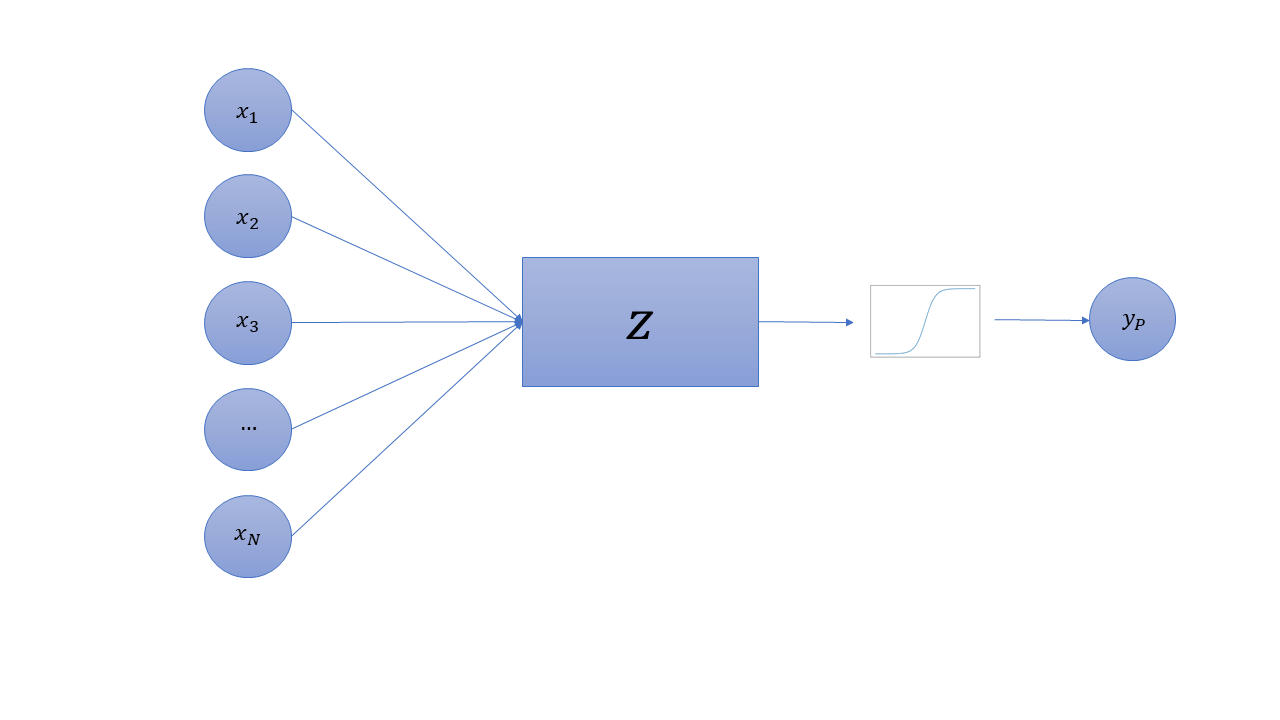
\includegraphics[width=\linewidth]{figures/Perceptron_network.png}
    \caption{A perceptron network whose inputs $x_1 ... x_N$ are each multiplied 
    by a learned set of corresponding weights $w_1 ... w_N$ and summed together in $z$. 
    The summed value is then passed through an activation function to get the final 
    output of the network.}
    \label{fig:Perceptron_network}
\end{figure}

where $y_{p}$ is our predicted output (e.g. class label), $x$ is our given input, $w$ is a learned scalar weighting term on $x$, $b$ is a learned scalar bias term on $x$ and $\sigma$ is a nonlinear activation function which rescales the output. Because we usually frame the classification problem such that a prediction of $0$ represents class $1$ and a prediction of $1$ represents class $2$, we typically apply a sigmoid activation function (Fig. \ref{fig:sigmoid}) since it limits the output to be between $0$ and $1$.

\begin{figure}
    \centering
    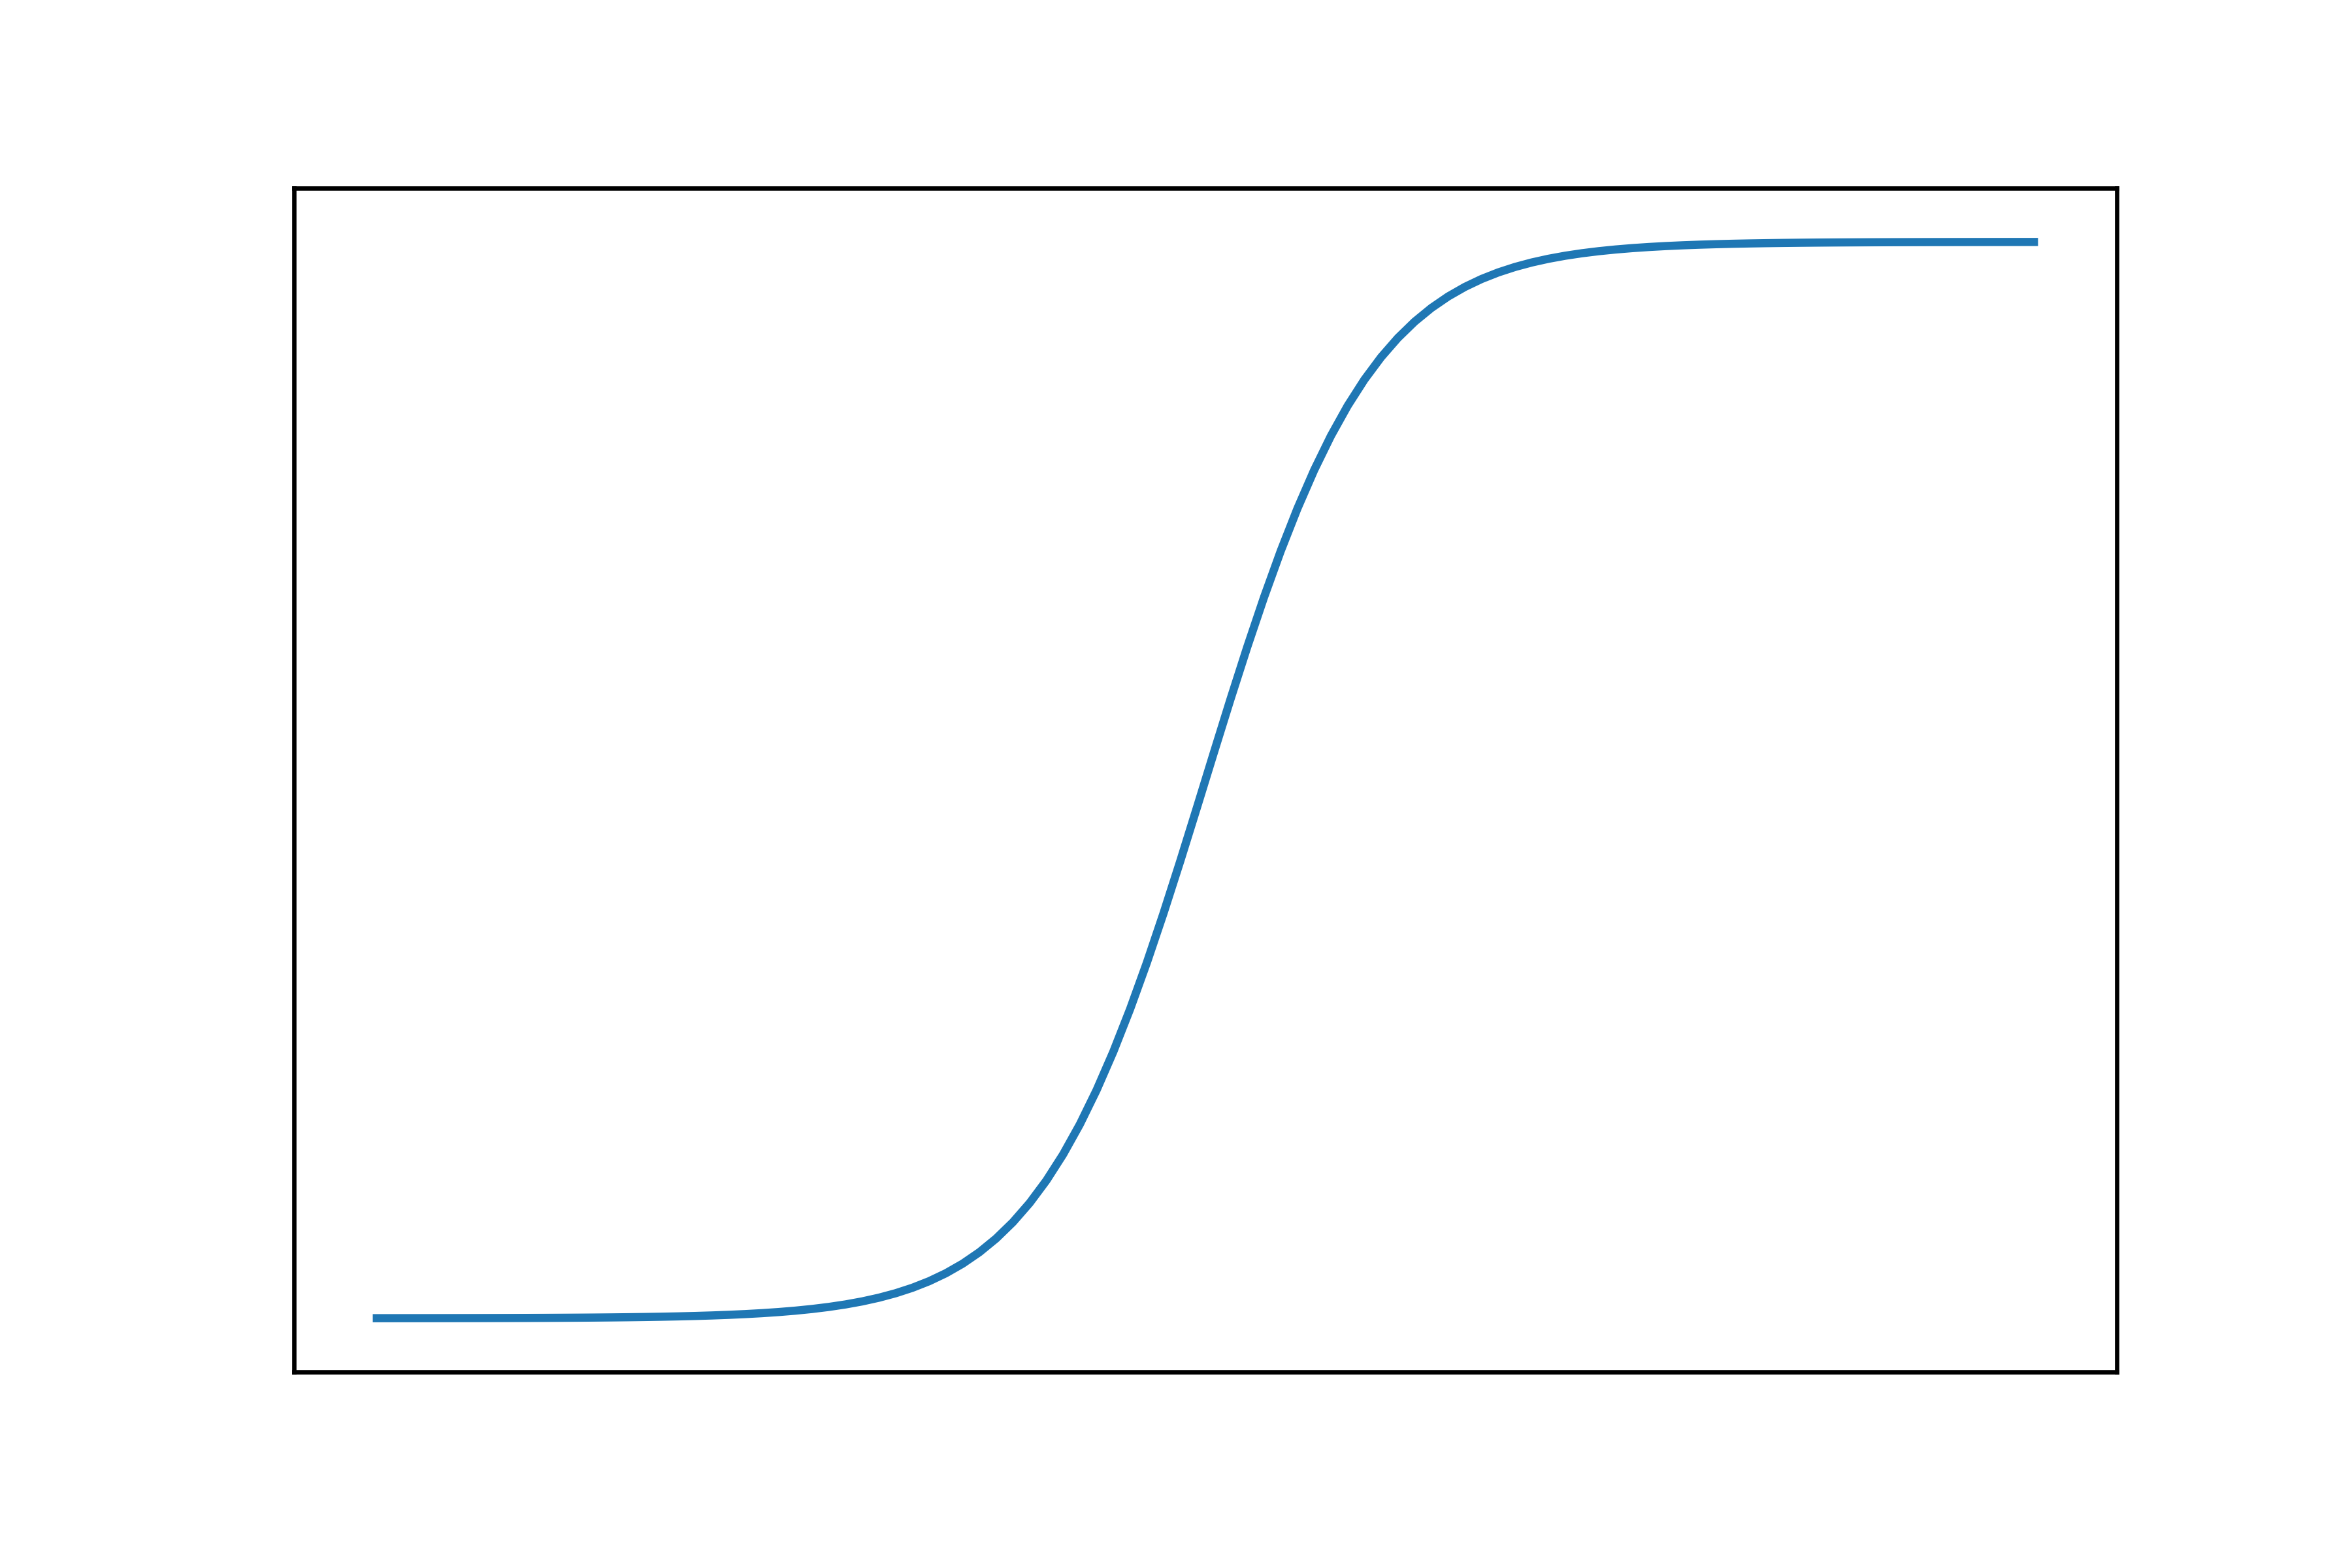
\includegraphics[width=\linewidth]{figures/sigmoid_function.png}
    \caption{A sigmoid activation function plotted over the input 
    range -10 to 10. Given an input over a pre-defined range, the 
    activation function will rescale the input to be between the range 
    of 0 to 1.}
    \label{fig:sigmoid}
\end{figure}

We also apply a nonlinear activation function in order to allow our perceptron to learn non-linear functions/features \cite{1811.03378}. All weights and biases are typically initialized randomly prior to training and there are many schemes for choosing the optimal initialization \cite{1704.08863}. In order to approximate more complicated functions, we can string together multiple perceptrons (neurons) in a layer where each neuron is fully-connected to the given input $x$ (i.e. every element in our input is multiplied by each weight of each neuron in our first layer)\cite{Goodfellow-et-al-2016}. To make a deep network, we can randomly initialize another layer of neurons (of arbitrary size) which takes as input the output from the previous first layer of neurons (illustrated in Fig.\ref{fig:deep_nn}). Additional layers can be added in perpetuity, although there are issues that can arise due to a vanishing gradient or hardware memory limitations \cite{1211.5063}. During training, weights and biases are updated according to the performance of the algorithm with respect to a loss function which describes how well the algorithm is performing with respect to the true value of each training sample\cite{1702.05659}. This loss function can take many forms, but most often a mean squared error is used

\begin{figure}
    \centering
    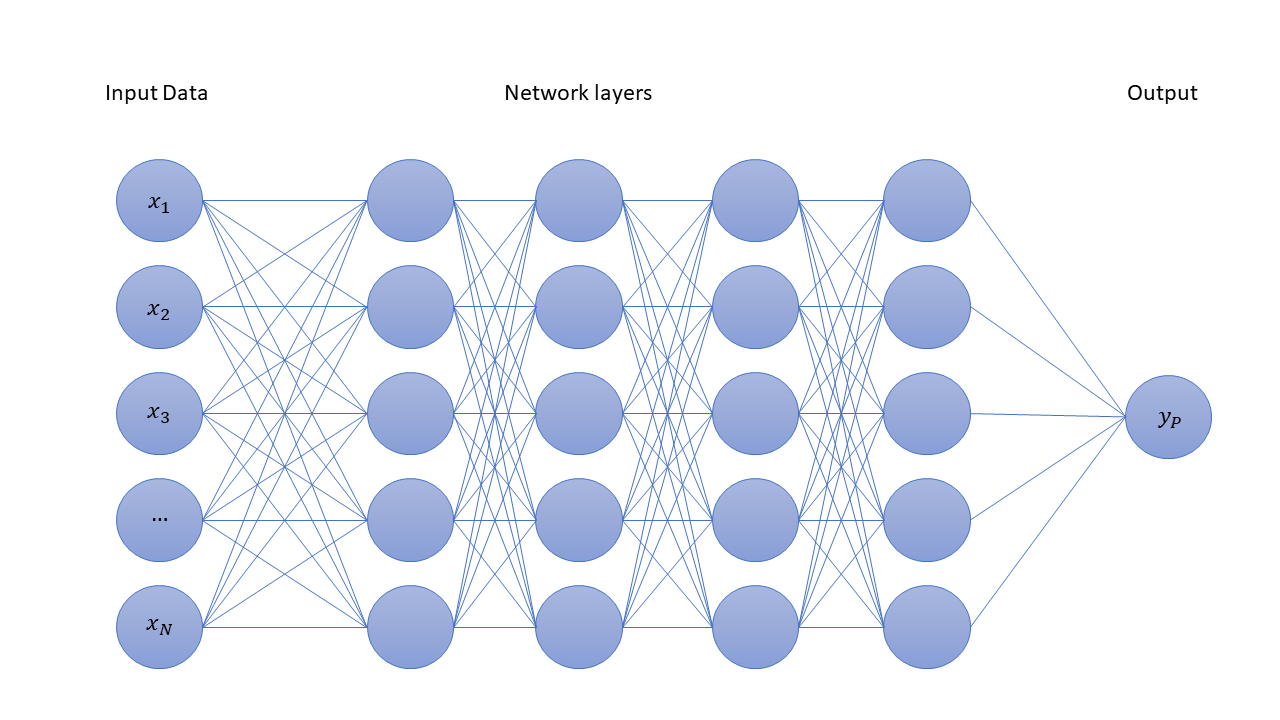
\includegraphics[width=17cm,height=20cm,keepaspectratio]{figures/DeepFullyConnectedNetwork.png}
    \caption{A deep fully-connected neural network. Inputs $x_1 ... x_N$ are given as input to the 
    first layer of the neural network and are fully-connected to every node in that layer. The outputs 
    of each node are then passed on to the next set of nodes in the next layer and are also fully-
    connected. The final layer passes through a final single node which determines the class/value 
    of the given input.}
    \label{fig:deep_nn}
\end{figure}

\begin{equation}
    L = \frac{1}{n} \sum_{i=1}^{n}(y^{l}_n-y^{t}_n)^2.
\end{equation}{}

%
% the loss function
%
Where $y^{l}_n$ is the neural network prediction and $y^{t}_n$ is the true value.
When the predicted label of nth training sample in the final layer $l$ $y^{l}_n$ is similar to the nth training sample true label $y^{t}_n$, the loss term approaches zero and is at a minimum. The reader's next question may rightly be, how does one go about choosing the right weights $w$ and biases $b$ for each neuron in the network? In other words, how much of an effect will changing $[w,b]$ have on the resulting loss function $L$. We can quantify the amount to change $[w,b]$ such that the loss is optimised through gradient decent\cite{1609.04747}. Specifically, we will be discussing a variant of gradient decent, stochastic gradient decent.

% Hebian theory "neurons that fire together, wire together"
%
% Stochastic gradient decent explanation
%
Stochastic gradient decent is an iterative algorithm used to find the global minimum (usually a local minimum is sufficient) of a function. Gradient decent essentially has two decisions it needs to make when choosing new weights and biases: what direction to go and by how much. The most straightforward way of getting this information is through the use of a derivative, specifically the gradient of the loss function $L$ defined as 

\begin{equation}
    g = - \gamma \nabla L(y^{l}),
\end{equation}{}

where $\gamma$ is a tunable step size scale factor (typically called the learning rate), $\nabla L(y^{l})$ is the gradient of the loss with respect to the weights and biases of the network and $g$ is a list of gradients corresponding to each weight and bias between the final output layer and the previous layer. The sign of the gradient for each weight and bias corresponds to the direction of in which to change the weights while the magnitude tells you how sensitive the loss function is to each weight and bias. If there are multiple neurons in the final layer of the network, the contributing gradients for each neuron in the final layer are summed in order to return a representative gradient with respect to all output neurons.

However, this only returns the gradients for the final output layer. In  order to appropriately update weights and biases in the previous layers we must propagate the gradient backwards. This process is better known as back propagation.

%
% Back prop explanation
%
In back propagation we use the computed gradient from the final layer and compute the gradient between that final layer gradient and the output from the second to last layer. The individual contributions from each neuron in the second to last layer are summed (same as was done in the final layer computation) and the gradients in the second to last layer are propagated back again to the third to last layer. Mathematically, we can define this process as the derivative of the loss with respect to the outputs of each layer $l$

\begin{equation}
    \nabla L(y^{l}) = \frac{\delta L}{\delta y^{(l)}}.
\end{equation}{}

Applying the chain rule and expanding this out for multiple layers we arrive at

% Need to add notation describing summation over each neuron in each layer
\begin{equation}
    \nabla L(y^{l}) = \frac{\delta z^{(l-m)}}{\delta y^{(l-m-1)}} \frac{\delta y^{(l-m)}}{\delta z^{(l-m)}} ... \frac{\delta z^{(l)}}{\delta y^{(l-1)}} \frac{\delta y^{(l)}}{\delta z^{(l)}} \frac{\delta L}{\delta y^{(l)}} 
\end{equation}{}

where the total derivative over all neurons in each layer may be quantified and applied to determine how much to shift each weight and bias in order to improve the overall loss of the neural network. This process is repeated until all weights and biases in the network have had their gradients computed. Ideally, we would compute the gradient over more than just one training sample, but rather the whole training set during each training iteration. However, computing the gradient over the whole network for all training samples is abhorrently expensive, so the training set is typically split up into mini-batches of samples in order to reduce the computational cost.

%
% Training best practices
%
\section{Training best practices (practical advice for the reader)}

I was commonly told when first wadding into the pool of deep learning that the practical implementation/training of deep learning models is largely a dark art. In this section, I would like to dispel that myth by offering some best practices when training any machine learning model.

%
% When in doubt, make more training data
%

\subsubsection{Training data size}
First off, when in doubt the more training data you make available to yourself, the better.
Time and again, during a large part of my thesis work, I would spend countless hours tuning and tweaking my neural network architecture only to run up against some insurmountable wall of impeded progress. Only then to increase the number of training samples by several factors and see a significant increase in performance. 

\subsection{Data pre-processing and augmentation}

\subsubsection{Data pre-processing}
Commonly, our input datasets are in a messy form. In order to help the network learn more efficiently, it is encouraged to perform some pre-procesing steps. It's important to do this because if our input data has large values over a wide range, and our network is trying to learn a mapping from input to prediction, the learned weights may also end up being very large. Large learned variable weights can lead to massive gradients which cause the network to update weights in large step sizes, making the whole network more unstable in the process. We can overcome this by normalising our input dataset to be between the range of zero to one 

\begin{equation}
    y = \frac{x - x_{\textrm{min}}}{x_{\textrm{max}}-x_{\textrm{min}}},
\end{equation}

where $y$ is our new normalised data, $x$ is our original unnormalised data, $x_{\textrm{min}}$ is our unnormalised data minimum value and $x_{\textrm{max}}$ is our unnormalised data maximum value. It can also be advantageous to rescale our input data to a standard normal distribution if our data has widely varying scales by applying 

\begin{equation}
    y = \frac{x - x_{\textrm{mean}}}{x_{\textrm{std}}},
\end{equation}

where $x_{\textrm{mean}}$ is the mean of our data and $x_{\textrm{std}}$ is the standard devitation of our data. In addition to rescaling our input data, we ocassionally need to also rescale our training labels. This is especially relevant if the activation function in our final neural network layer is fixed to be between some values. For example, if we were using a sigmoid activation function where the values of the output of the sigmoid are only allowed to be between zero and one, then we would also want our training label values to lie between zero and one since the network would not be able to produce values outside of that range.

\subsubsection{Data augmentation}

Neural networks can sometimes be composed of hundreds, thousands, even million of parameters to be tuned during training. Given the massive number of parameters, many complex networks require an equally massive number of training samples. But, what do you do if you are only given a limited number of training samples? This is where data augmentation comes to the rescue. In order to generate more training data, we can apply simple shifts to the existing limited dataset and greatly expand the number of training samples. This can be accomplished through many of the following methods:

\begin{itemize}
    \item Translation: Shift the input data sample in the x/y/z direction.
    \item Rotation: Rotate data about a fixed point.
    \item Cropping: Choose a random subset of the input sample, cut out all data outside of subsection, rescale cropped data to original input size.
    \item Gaussian noise: Add varying amounts of Gaussian noise in order to simulate poor quality signals.
\end{itemize}

%
% The purpose of Validation
%
\subsection{Validation}
In order to understand how well your model is performing with respect to the training data, one may plot the resultant average output of the loss function as a function of the number of training iterations. Ideally, we would like the loss to rapidly decrease and to then flatten out. Although this will give us an indication of how well the network is performing on the training set, it does not inform us as to how well the model will generalize to a novel testing set. In order to quantify the generalization ability of the network, we may set aside a small portion of the training set prior to training as a validation set. During training, we can temporarily freeze the weights and run the validation set through the model in order to compute a validation loss. 

If we plot both the validation loss and the training loss as a function of time, we again ideally would like to see both curves decrease as a function of training iteration and then level out. However, if we see that the training curve initially decreases and then continues to decrease while the validation curve initially decreases and then subsequently increases we may say that the model has overfit the training data. Overfitting the training set generally indicates that either our model is too complicated and has essentially memorized the training set or that we do not have enough training data to sufficiently cover the entire parameter space. Overfitting can be mitigated by increasing the training set size, adding dropout connections (see Regularization sub section), early stopping of the training run or reducing the complexity of the neural network.

If on the other hand we see that the validation loss decreases far quicker than the training loss then we may say that the model has underfit the data, which is generally an indication that the model needs to have an increased capacity.

%
% Regularization techniques
%
\subsection{Regularization}

%
% Dropout
%
Regularization is used to help prevent a machine learning model from overfitting the the training data. One of the easiest regularization techniques to implement is that of dropout. Dropout may be implemented across most types of neural network layers (i.e. fully-connected, convolutional filters, etc.) and rarely have any adverse effect on training. During training, if dropout is implemented a subset of the neurons in a layer will be switched off and not used when the gradient is computed and backpropogated through the network for a given training iteration. The percentage of neurons in a layer to switch off is a tunable parameter, though typically it is best to set a value of no more than $50\%$. Dropout effectively forces the neurons in a dropout layer to be able to identify multiple features, rather than to focus a small subset.

%
% Batch noramlization
%
Batch normalization is motivated by the same principle that standard normalization of input to a neural network is motivated. We want to reduce the space over which the neural network has to search. As such, batch normalization is essentially a normalization of the output of individual layers within a neural network to be between zero and one. This normalization prevents weights or biases from becoming too large. It is computed by normalization of the current layer according to the mean and standard deviation of the output of the previous layer and the subsequent rescaling through two learned variables ($\alpha$ and $\beta$) and is formalised as 

\begin{equation}
    z_n = \alpha \hat{z}_n + \beta,
\end{equation}{}

where $\alpha$ is a learnable parameter, $\beta$ is a learnable parameter and $\hat{z}_n$ is calculated by 

\begin{equation}\label{eq:batch_norm}
    \hat{z}_n = \frac{1}{n} \sum_{i=1}^{n} \frac{z_n - \mu}{\sigma^{2} + \epsilon},
\end{equation}{}

where $z_n$ is the output of the neural network layer summed over all outputs in the batch of that layer, $[\mu,\sigma]$ are the mean and standard deviation respectively of the batch of previous layer outputs introduced to the network and $\epsilon$ is a small constant. If it turns out that the application of batch normalization is not optimal, then the network may undo the above normalization in e.q. \ref{eq:batch_norm} through the optimization of $[\alpha,\beta]$ in each layer.

\subsection{Hyperparameter optimization}

In many instances, after we have spent all our time cleaning the data, 
choosing a model to solve our problem and then finally 
training our model, we find that the most tedious and 
time consuming part of the whole endeavor is all those 
pesky model hyperparameters. In this sub section, I will 
describe three approaches used in this thesis to optimize 
hyperparameter choices.

\subsubsection{Random Search}
Probably the simplest of the three approaches random search 
seeks to choose model hyperparameters based off of a 
predefined prior distribution for each hyperparameter. 
The user may define whatever distribution they prefer 
whether that be a multivariate Gaussian distribution 
or a uniform distribution so long as the bounds of the 
distribution chosen are within reason.

\subsubsection{Grid Search}

Grid search is marginally more complicated. In a grid 
search approach we define both an upper and a lower limit 
for each hyperparameter. Additionally, we define a step 
size by which we will increase the the hyperparameter 
value after each model evaluation (much like steps 
on a ladder). Each of these hyperparameter 
ladders are iterated over in an N dimensional grid, 
where N is representative of N hyperparameters 
describing the model. 

\subsubsection{Gaussian Process Bayesian hyperparameter optimization}

Bayesian hyperparamter optimization aims to minimize (or maximize) some 
objective function. In this case, we aim to learn an 
approximate surrogate model for an objective function which 
describes the loss function space and to minimize the value of the 
loss function output. The dimensionality of the search space 
is parameterized by the number of neural network hyperparameters being optimized 
and does not usually perform well past 20 dimensions. Gaussian process 
regression is used in order to minimize the uncertainty on the surrogate model estimate 
. We then use an acquisition function to sample from the approximate 
surrogate model to determine the next set of hyperparameters to use 
during the next round of neural network training \cite{1807.02811}.

In practice, we first choose an initial set of hyperparameters 
to use in order to train the network. This can either be randomly chosen 
from a reasonable prior, or a best guess from the practitioner. 
Next, the neural network is trained a pre-defined number of 
training iterations and the network loss function output value 
is given as input to the Bayesian optimization algorithm. The Bayesian 
optimization algorithm then updates its surrogate model 
based off of this new loss value from the neural network 
given the hyperparameters used and a new set of 
hyperparameters is chosen by an aquisition function based 
informed by the Gaussian process regression surrogate model. 
The above process is repeated for N user pre-defined iterations.
%
% Note, fill out this section using the following resources:
% https://arxiv.org/pdf/1807.02811.pdf
% https://towardsdatascience.com/tl-dr-gaussian-process-bayesian-optimization-5e66a014b693

\section{Convolutional Neural Networks}

\ac{CNN}s were first made popular in the late 1980s to early 1990s 
and one of the most famous examples is that of the LeNet archetecture 
made by Yann LeCunn in 1998 \cite{726791}. In his paper, LeCunn 
illustrated that \ac{CNN}s outperformed other simpler 
techniques like K Nearest Neighbor and fully-connected 
neural networks on a variety of image recognition 
tasks. In recent years \ac{CNN}s have been applied to 
many more domains including image object detection, 
fraud identification, healthcare analysis and many 
others. In this section I will explain how \ac{CNN}s work, 
mechanisms for improving \ac{CNN} performance, and 
why they are so powerful for image based tasks.

\subsection{The convolutional filter}

% 
% Really need to rewrite section about odd filters ...
% 
The basic building block of a \ac{CNN}, convolutional 
filters are analogous to neurons in a standard fully-connected 
neural network. A convolutional filter is typically made up of 
an $N \times N$ matrix of any size that the user wants( for illustraed 
exmample, see Fig.\ref{fig:cnn_filter_illustration}). Normally, 
the dimensions are of odd size because all pixels from the input 
to the filter are enforced to be centered around the output 
of the filter. This effectively acts to anchor the output 
of the filter, in a sense acting to interpolate all 
the anchor pixels neighboring pixels. Without using odd size filters, distortions 
across multiple layers can cause issues, though are not impossible 
to overcome through added network complexity.

\begin{figure}
    \centering
    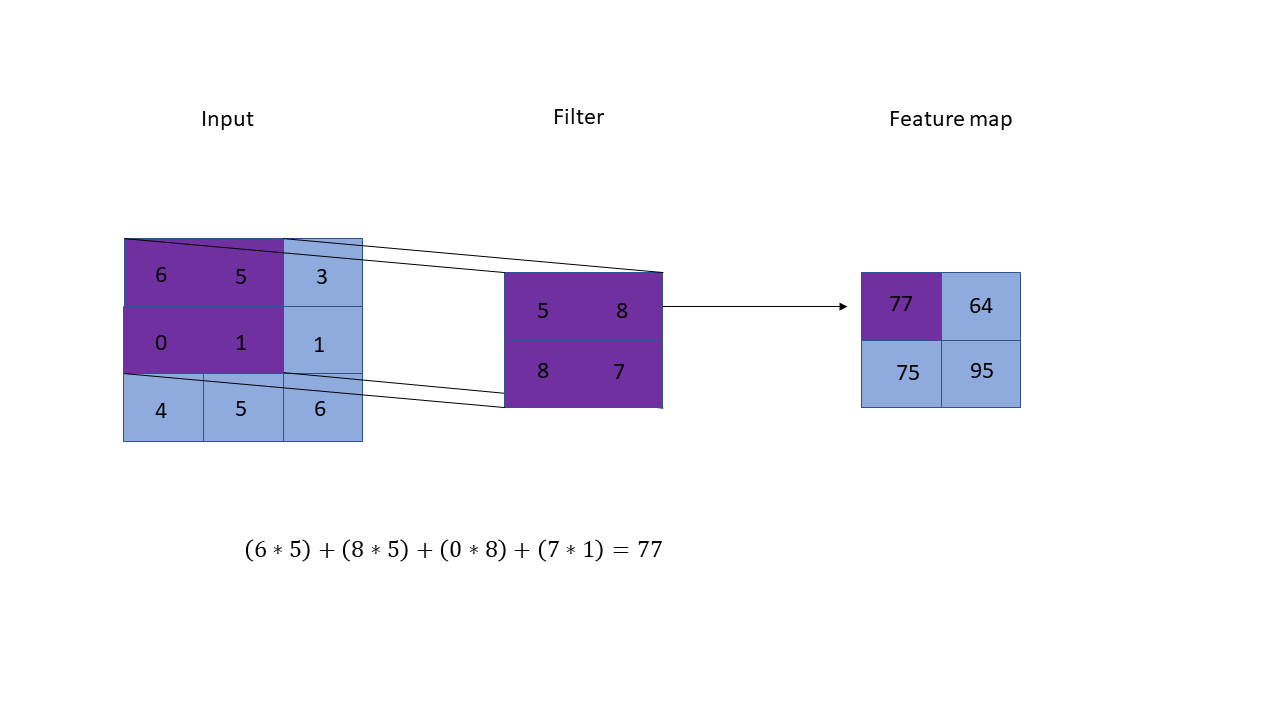
\includegraphics[width=17cm,height=20cm,keepaspectratio]{figures/cnn_filter_illustration.png}
    \caption{An illustration of a simple \ac{CNN} filter. The filter is a $2 \times 2$ filter randomly initalised with a set of weights for each dimension. Each filter weight is multiplied by the corresponding input dimension over which it is currently covering. All multiplied values are then summed together to produce the output of the filter. The filter slides over one element (if stride is set to 1) and the computation is done again until the whole input space has been covered.}
    \label{fig:cnn_filter_illustration}
\end{figure}

Values in the $N \times N$ matrix of the filter are initialised 
randomly with an added bias term. The initialised values in the 
filter are the weights of the filter. During training, the filter is 
convolved with its given input where each element in the filter 
is multiplied by the corresponding overlapping element in the 
input. All the multiplied values are then summed together to produce 
the output of the filter. A bias term is then added to the 
output. We the slide the filter over by 1 column and repeat 
the convolution process until the edge of the filter reaches 
the last column of the input. We then slide the filter back to 
the 1st column of the input and down one row and repeat 
the convolution process on all columns again. This is done 
until we have convolved the filter over the whole input.

\subsection{Pooling layers}
Pooling is a form of regularization and acts to choose 
the most important features in each convolution of a filter. 
We do this because many times \ac{CNN} filters will focus 
on minute detailed information, but loose sight of the 
bigger picture. This means that small changes in the 
input, will have large effects on the filter. In order to 
combat this, pooling acts to downsample the input, making 
it more ``fuzzy'' in the process, forcing the model 
to learn broader features.
This is done by taking the maximum value over all elements 
in a convolution and discarding all other values. 

\subsection{Striding}
In addition to pooling, another form of regularization is 
striding. Striding determines the number of pixels a 
convolutional filter moves after each convolution 
is performed. Standard techniques nominally employ 
a stride of 2. Additionally, because we are skipping 
over some parts of the input when sliding the filter, 
striding can act to reduce the total memory usage of a 
\ac{CNN}.

\subsection{The fully-connected layers}

Following the convolutional filter layers, we now 
have to convert the output of the CNN to predict 
a discrete set of classes or regress on some parameter. 
If performing binary classification, one could simply 
make the last layer of the \ac{CNN} two 1D convolutional 
filters, however this is usually not what is normally 
done. Typically, a flattening operation is applied 
to the last convolutional layer where the concatenated 
feature maps from the previous layer's filters 
are flattened into a 1D string of elements. This 1D 
string of elements are then given as input to 
a fully-connected layer of neurons. One can then add 
additional fully-connected layers and a final 
layer equivalent to either the number of classes to 
predict, or the number of parameters to regress on. 
A logical question may be why add this extra 
fully-connected complication? First and least 
informative answer is that it just what has 
always been done since time immortal. Second 
slightly more intuitive answer is that we want 
to unify the learned features across all 
\ac{CNN} filters and use those features to learn 
how to either classify or regress.


\section{Conditional Variational Autoencoders}

In this section I will describe the network architecture of a 
\ac{CVAE}. This will be done by first describing an \ac{AE} network, then 
a \ac{VAE} network and finally a \ac{CVAE} network.

%
% Autoencoders
%
\subsubsection{Autoencoders}

An \ac{AE} is 
comprised of two neural networks called an 
encoder and decoder. The encoder is given an input 
from a pre-generated training set (in this case, lets assume 
we are dealing with the MNIST dataset). The output of the 
encoder network is typically smaller than the dimension of 
the input, essentially forming a bottleneck. 
We call the output of the encoder the latent space representation. 
The predicted numbers from the encoder representing the latent 
space are then given as input to the decoder network. The 
decoder then tries to reconstruct the given input to the 
encoder network (Fig.\ref{fig:autoencoder_diagram}). We measure how well the network is performing 
through a loss function given as 

\begin{figure}
    \centering
    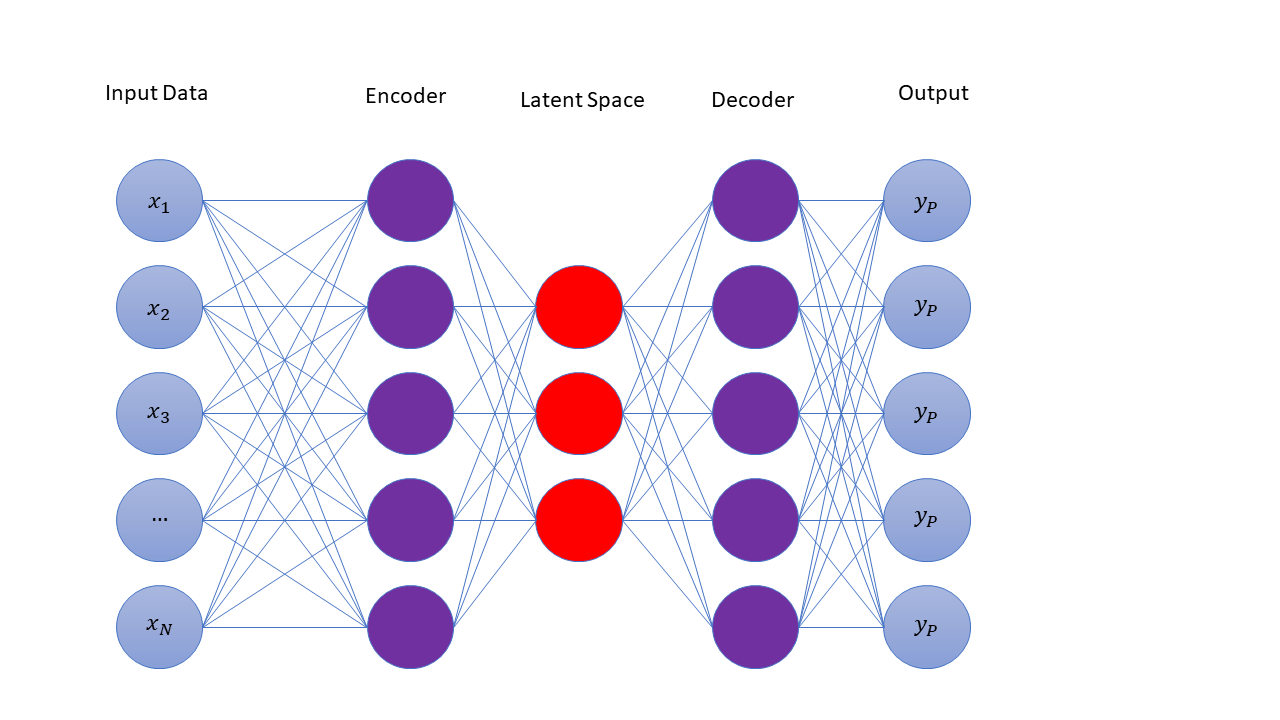
\includegraphics[width=19cm,height=20cm,keepaspectratio]{figures/autoencoder_diagram.png}
    \caption{An autoencoder network composed of two neural networks defined as the encoder 
    and the decoder networks. Here, both networks are represented as fully-connected networks, but could also be any number of other network architectures such \ac{CNN}s and \ac{LSTM} networks. The encoder network takes as input a set of data and compresses the data  
    through a bottleneck called the latent space. The latent space is then given as input to the decoder network which tries to reconstruct the given input $x_1 ... x_N$.}
    \label{fig:autoencoder_diagram}
\end{figure}

\begin{equation}
    l(f(x)) = \sum_k{(f(x)_k - x_k)^2},
\end{equation}

where $f(x)_k$ is the output from the decoder network on the 
kth training/testing sample of the \ac{AE} and $x_k$ is the 
kth training/testing sample. During training, $f(x)_k$ is trained 
to be as similar to $x_k$ as possible in order to minimise 
$l(f(x))$. The lower the value $l(f(x))$ is, the better the network 
is performing. The loss $l(f(x))$ is then backpropagated through 
the network adjusting the weights and biases in order to  
further minimise the loss.

\ac{AE}s can be used across a variety of applications including: 
dimensionality reduction \cite{6910027}, image denoising \cite{NISHIO2017e00393},
feature extraction \cite{7965877} and many others. Although powerful, 
one of the limitations of an \ac{AE} is the way it represents the 
latent space. Within the context of \ac{AE}s as content generators 
the reader would be forgiven for thinking that, if properly trained, 
one could just simply sample from the latent space uniformly 
in order to generate unique content. However, due to the fact 
that the network is not required to distribute learned latent 
space representations during training (features are allowed 
to be encoded anywhere in the latent space), it is not 
guaranteed that latent space samples will be from a 
learned part of the latent space.

%
% Variational autoencoders
%
\subsubsection{Variational Autoencoders}

We can overcome this, through the use of a \ac{VAE} (see illustration in 
Fig.\ref{fig:simple_vae}. 
A \ac{VAE} is nearly identical to an \ac{AE}, except for 
the main differences arising from how the latent space 
is represented and how the loss function is constructed. 
If we go back to our original problem, where the encoder is given 
a sample MNIST digit image; instead of having the encoder network 
output a single predicted value for each dimension in the 
latent space, we now have it output both a predicted 
mean and standard deviation value describing a Gaussian 
for each dimension. Samples are then drawn from the the 
predicted distributions and given as input the decoder network. 
The decoder network produces estimates trying to reconstruct 
the given input to the encoder network. The loss for 
a \ac{VAE} is also slightly different and is represented 
as 

\begin{figure}
    \centering
    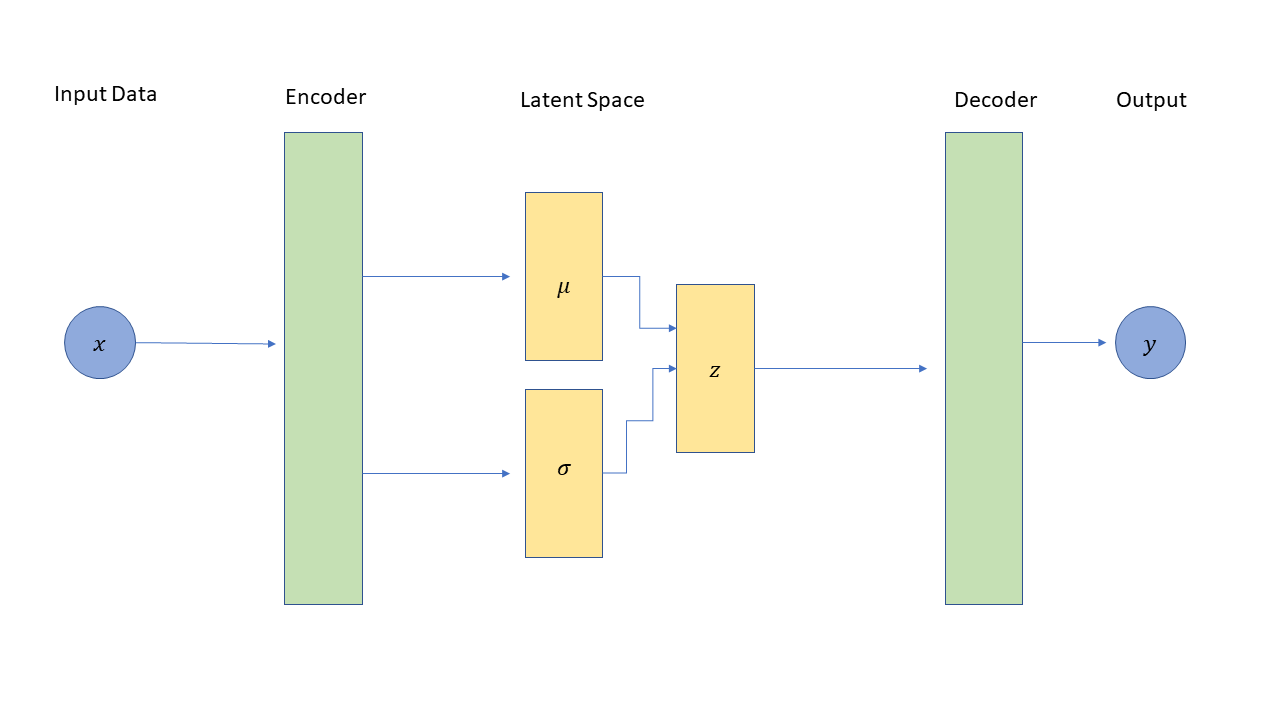
\includegraphics[width=16cm,height=20cm,keepaspectratio]{figures/simple_vae_diagram.png}
    \caption{A simplified diragram of a variational autoencoder network. The input data $x$ is passed to the encoder neural network which produces predictions on the means $\mu$ and standard deviations $\sigma$ of multi-variate Gaussian distributions describing the latent space. Samples are drawn from the predicted distributions $z$ in order to get samples from the latent space. These latent space samples are then passed to the decoder network which attempts to reconstruct the given input $x$.}
    \label{fig:simple_vae}
\end{figure}

\begin{equation}
    l(f(x)) = \sum_k{ (f(x)_k - x_k)^2 + 
    D_{\textrm{KL}}[N(\mu_k, \sigma_k), N(0, 1)]},
\end{equation}

where $f(x_k)$ is the predicted output from the decoder, $x_k$
is the given input to the encoder, $D_{\textrm{KL}}$ is the \ac{KL} divergence 
between latent space samples from predicted Gaussians $N(\mu_k, \sigma_k)$ 
and samples from a mean zero unit variant Gaussian 
distribution $N(0,1)$. 

We can derive this loss function by first assuming that we 
want to approximate the optimal latent space posterior 
representation using a neural network. I will be directly following a 
similar derivation done in \cite{1907.08956}. We can define the 
difference between the approximate and the truth as 

\begin{equation}
    D_{\textrm{KL}}(q_{\theta}(z|x_k) || p(z|x_k)) = -\int q_{\theta}(z|x_k) \log(\frac{p(z|x_k)}{q_{\theta}(z|x_k)}) dz,
\end{equation}

where $q_{\theta}(z|x_k)$ is the approximate posterior of the 
latent space and $p(z|x_k)$ is the optimal representation. 
We can then substitute Bayes theorem in for the truth 
$p(z|x_k)$ as 

\begin{equation}
    D_{\textrm{KL}}(q_{\theta}(z|x_k) || p(z|x_k)) = -\int q_{\theta}(z|x_k) 
    \log(\frac{p(x_k|z) p(z)}{q_{\theta}(z|x_k) p(x_k)}) dz. 
\end{equation}

We now separate out the division using the laws of logarithms and 
distribute the integrand

\begin{equation}
    D_{\textrm{KL}}(q_{\theta}(z|x_k) || p(z|x_k)) = -\int q_{\theta}(z|x_k) 
    \log(\frac{p(x_k|z) p(z)}{q_{\theta}(z|x_k)}) - \log(p(x_k)) dz. 
\end{equation}\

\begin{equation}
    -\int q_{\theta}(z|x_k) 
    \log(\frac{p(x_k|z) p(z)}{q_{\theta}(z|x_k)}) +
    \int q_{\theta}(z|x_k) \log(p(x_k)) dz. 
\end{equation}\

Due to the fact that $q_{\theta}(z|x_k)$ is a probability distribution, 
we can assume that integral of $q_{\theta}(z|x_k)$ is equal to 1, 
further simplifying the equation. We also know that by definition the KL 
divergence must be greater than zero, so we can set the whole 
equation to be greater than or equal to zero

\begin{equation}
    -\int q_{\theta}(z|x_k)
    \log(\frac{p(x_k|z) p(z)}{q_{\theta}(z|x_k)})dz +
    \int \log(p(x_k)) \geq 0. 
\end{equation}\

Since $\log(p(x_k))$ is a constant, we can remove the integrand 
on the right-hand side

\begin{equation}
    -\int q_{\theta}(z|x_k)
    \log(\frac{p(x_k|z) p(z)}{q_{\theta}(z|x_k)})dz +
    \log(p(x_k)) \geq 0.
\end{equation}

Moving the integral over to the right-hand side we get 

\begin{equation}
    \log(p(x_k)) \geq \int q_{\theta}(z|x_k)
    \log(\frac{p(x_k|z) p(z)}{q_{\theta}(z|x_k)})dz.\label{eq:lookbackKL}
\end{equation}

Applying rules of logarithms yet again, we can now expand 
out the above equation into 

\begin{equation}
    \log(p(x_k)) \geq \int q_{\theta}(z|x_k)
    [\log(p(x_k|z)) + \log(p(z)) - \log(q_{\theta}(z|x_k))] dz.
\end{equation}

We can now recognize that the expression on the right 
is equivalent to the expectation value over the log 
terms given as 

\begin{equation}
    \log(p(x_k)) \geq E_{\sim q_{\theta}(z|x_k)} 
    [\log(p(x_k|z)) + \log(p(z)) - \log(q_{\theta}(z|x_k))]
\end{equation}

\begin{equation}
    \log(p(x_k)) \geq E_{\sim q_{\theta}(z|x_k)} 
    [\log(p(x_k,z)) - \log(q_{\theta}(z|x_k))].
\end{equation}

Taking a small look back to equation (\ref{eq:lookbackKL}), 
and using the rules of logarithms we can rewrite it as 

\begin{equation}
    \log(p(x_k)) \geq \int q_{\theta}(z|x_k)
    \log(\frac{p(z)}{q_{\theta}(z|x_k)})dz + 
    q_{\theta}(z|x_k) \log({p(x_k|z)}) dz
\end{equation}

We can now see clearly that the first expression on the 
right-hand side of the above inequality is equivalent to the 
negative \ac{KL} divergence between our approximate latent space 
representation $q_{\theta}(z|x_k)$ and our prior on 
the latent space $p(z)$

\begin{equation}
    \log(p(x_k)) \geq - D_{\textrm{KL}}(q_{\theta}(z|x_k) || p(z)) + 
    q_{\theta}(z|x_k) \log({p(x_k|z)}) dz. 
\end{equation}

Conveniently, we also see that the right most term on the 
right-hand side of the inequality can be approximated as the 
expectation value of the log probability of the data $x_k$ 
given $z$

\begin{equation}
    \log(p(x_k)) \geq - D_{\textrm{KL}}(q_{\theta}(z|x_k) || p(z)) + 
    E_{\sim q_{\theta}(z|x_k)}[ \log({p(x_k|z)})].\label{eq:vae_loss}
\end{equation}

And there we have it, the loss function for the \ac{VAE}! 
The whole expression to the right of the inequality
is typically denoted as the \ac{ELBO} because it puts a 
lower bound on the log likelihood of the data $log(p(x))$. For 
practical purposes, expectation value on the right can be computed analytically 
by performing the mean squared error between predictions on $x_k$ given 
latent space samples from $q_{\theta}(z|x_k)$ and the true 
$x_k$ values give as input to the encoder. The KL term acts to constrain 
the form of the approximate posterior $\log(p(x_k))$ according to 
a chosen prior on the latent space representation $p(z)$ across the whole input 
parameter space. The KL is essentially a regularization factor which helps 
the model to learn a well-formed latent space and reduce the likelihood 
of overfitting to the training data. $p(z)$ is nominally chosen to be 
represented as a mean zero, unit variant Gaussian distribution. Samples 
are drawn from predicted means and standard deviations from the 
encoder $q_{\theta}(z|x_k)$ and samples are also drawn from a unit variant 
Gaussian representative of the prior $p(z)$. We can then 
analytically compute the KL divergence value. The results from the KL 
and the ELBO calculations are then summed together and the whole term is 
minimized through backpropogation.

%
% reparameterization trick
%
\subsubsection{The reparameterization trick}

First proposed by Kingma et al. in their seminal \ac{VAE} 
paper \cite{1312.6114}, the reparameterization trick acts to 
solve a problem that we now have with the above derived loss 
function for the \ac{VAE}. That problem being that we cannot 
backpropagate the gradient computed with respect to the loss through 
a random node. The random node referred to is the latent space node 
given as input to the decoder which we define as 

\begin{equation}
    z = \mu + \sigma,\label{eq:before_repar} 
\end{equation}

where $z$ are samples from our latent space, $\mu$ are predicted means 
describing multivariate Gaussians and $\sigma$ are predicted standard deviations. 
We can prove that the above equation is nondifferentiable by first rewriting 
the expression as an expectation value

\begin{equation}
    E_{p(z)}[f(z)],
\end{equation}

If we then go to compute the gradient of the expectation value 
(which we would normally do when updating the weights in the 
\ac{VAE}), then we get the following expression

\begin{align}
    \nabla_{\theta} E_{p(z)}[f_{\theta}(z)] = \nabla_{\theta} \int p(z) f_{\theta}(z) dz\\ 
    = \int p(z) \nabla_{\theta} f_{\theta}(z) dz\\
    = E_{p(z)}[\nabla_{\theta} f_{\theta}(z)]
\end{align}

where it is shown that the gradient of the expectation value 
of $f(z)$ is equivalent to the expectation value of the gradient 
of $f(z)$, which is easily computed since the probability distribution 
is not a function of weights and biases $\theta$. However, if the probability distribution 
were a function of $\theta$, which it is since the latent space is produced 
by the encoder network which is itself a function of weights $\theta$, then 
we see the following happen when taking the gradient of the 
expectation value

\begin{align}
    \nabla_{\theta} E_{p_{\theta}(z)}[f(z)] = \nabla_{\theta} \int p_{\theta}(z) f_{\theta}(z) dz\\
     = \int \nabla_{\theta}  p_{\theta}(z) f_{\theta}(z) dz\\\
     = \int  p_{\theta}(z) \nabla_{\theta} f_{\theta}(z) dz + \int  f_{\theta}(z) dz \nabla_{\theta} p_{\theta}(z) dz\\
     = E_{p_{\theta}(z)}[ \nabla_{\theta} f_{\theta}(z)] + \int  f_{\theta}(z) dz \nabla_{\theta} p_{\theta}(z) dz\\
\end{align}

Although the first summation term is again easily computed, we now are 
left with a particularly intractable integral on the right-hand side.
Monte Carlo methods do allow us to randomly sample from $p_{\theta}(z)$, but 
they do not guarantee that we may take its gradient. 
We are now left with a bit of problem in how we are expected to compute the integral.
However, if we make a small change to equation (\ref{eq:before_repar}) 
by scaling the standard deviation by a deterministic value, we will 
see how this then solves our intractable integral problem. 

If we parameterize this deterministic value as samples drawn 
from a mean zero, unit variant Gaussian distribution 
$\sim N(0, 1)$ which we will denote as 

\begin{equation}
    \epsilon = N(0, 1).
\end{equation}

Then we can rewrite equation (\ref{eq:before_repar}) as 

\begin{equation}
    z = \mu + \sigma \epsilon.
\end{equation}

we'll now simplify the expression to be a function 
$g$ which is parameterized by $\epsilon$ and $x$, 
where $x$ is representative of $\mu$ and $\sigma$

\begin{equation}
    z = g_{\theta}(\epsilon, x).
\end{equation}

rewriting as an expectation value 

\begin{equation}
    E_{p_{\theta}(z)}[f(z^{(i)})] = E_{p(\epsilon)}[
    f(g_{\theta}(\epsilon, x^{(i)}))].
\end{equation}

Taking the gradient with respect to the weights 
and biases of the network $\theta$ we get 

\begin{align*}
    \nabla_{\theta} E_{p_{\theta}(z)}[f(z^{(i)})] = \nabla_{\theta} E_{p(\epsilon)}[
    f(g_{\theta}(\epsilon, x^{(i)}))]\\
    = E_{p(\epsilon)}[ \nabla_{\theta}
    f(g_{\theta}(\epsilon, x^{(i)}))].
\end{align*}

where we see that indeed we can take the gradient 
of $f(g_{\theta}(\epsilon, x^{(i)}))$ since 
$g_{\theta}(\epsilon, x^{(i)})$ is differentiable 
with respect to $\theta$. We can now just simply 
randomly Monte Carlo sample in order to analytically 
calculate $\nabla_{\theta} E_{p_{\theta}(z)}[f(z^{(i)})]$.

%
% conditional variational autoencoders
%
\subsubsection{Conditional Variational Autoencoders}

Through our rigorous derivations in the previous sections 
we have now formulated a loss function which can be trained 
to maximize the expected log probability of our 
decoder's prediction, while also regularizing its
model for the latent space to a smooth representation. 
However, there are some minor drawbacks to the \ac{VAE} 
which make it unsuitable for some generative tasks. 

For example, if we wanted to train our \ac{VAE} on 
the fashion MNIST dataset \cite{DBLP:journals/corr/abs-1708-07747}, 
a database of digit images representative of various classes 
of fashion items (shoes, shirts, pants), in order to 
generate new images of fashion items we would run into 
a problem. This problem is most clearly illustrated when 
taking a closer look at equation (\ref{eq:vae_loss}). In 
equation (\ref{eq:vae_loss}), it can seen that the encoder 
is solely conditioned on inputs from the training space 
$x_k$, but not on what class/type of image $x_k$ is. Similarly, 
the decoder is solely conditioned on the latent space $z$. In order 
to produce a particular class of input from the decoder, we would have 
to know which part of the latent space each class lives and to then 
draw from the location of the latent space that our class of 
interest resides. Knowledge of class location is infeasible to obtain 
after training because the KL 
divergence term in equation (\ref{eq:vae_loss}) enforces that 
on average across the whole training set that the predicted 
latent space locations are representative 
of a mean zero Gaussian distribution, but does not constrain where 
individual classes of input may reside.

The natural question then arises, is it possible to condition 
the network on classes of interest? It turns out that this is 
possible to do by making a minor update to the 
\ac{VAE} loss in equation (\ref{eq:vae_loss})

\begin{equation}
    \log(p(x_k)) \geq - D_{\textrm{KL}}(q_{\theta}(z|x_k,c) || p(z,c)) + 
    E_{\sim q_{\theta}(z|x_k,c)}[ \log({p(x_k|z,c)})].
\end{equation}

Here, we now condition the encoder $q_{\theta}(z|x_k,c)$ on both 
the training images $x_k$ and the class of said images $c$ (see Fig.\ref{fig:simple_cvae}). In the decoder 
$p(x_k|z,c)$ we condition on samples from the latent space $z$ and the 
class $c$. For classification purposes, the class is usually 
parameterized as a single scalar number which is appended to the input to 
the encoder and decoder networks. Now, if we wanted to use the decoder 
as a fashion image generator, we would only simply need to draw a 
random sample from the latent space, choose a class number, and then 
feed both as inputs to the decoder network. 

\begin{figure}
    \centering
    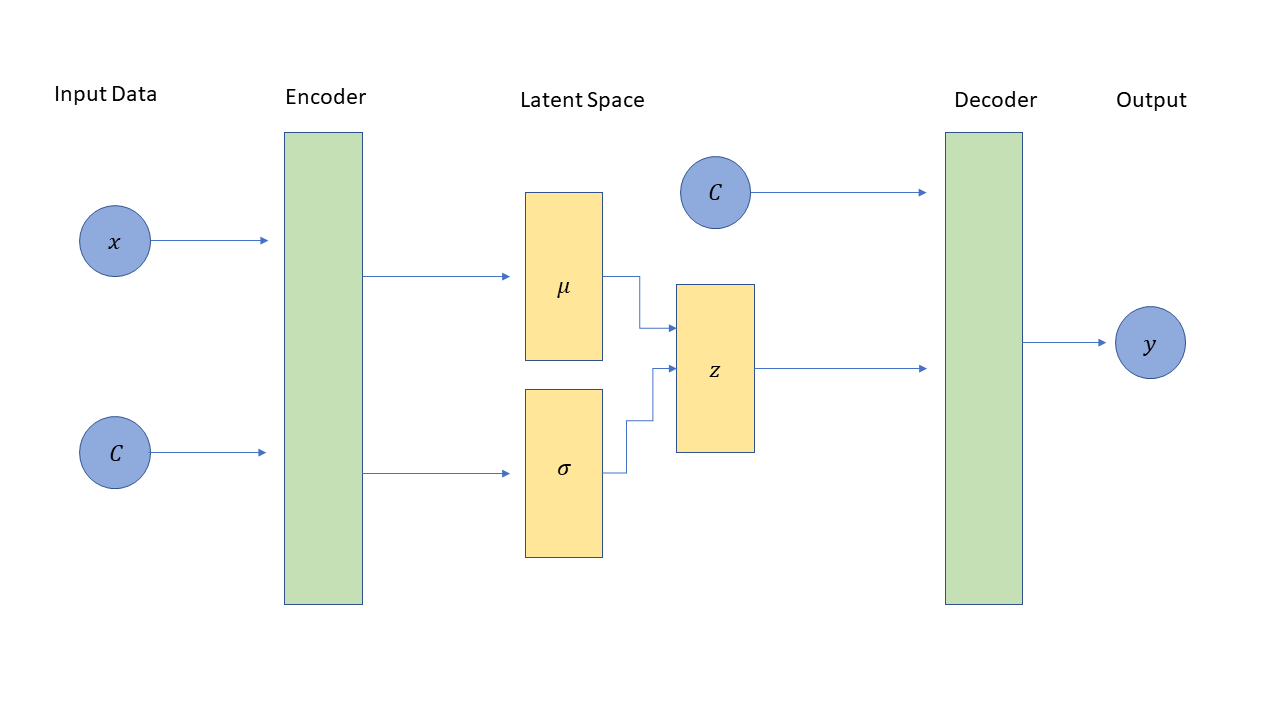
\includegraphics[width=16cm,height=20cm,keepaspectratio]{figures/simple_cvae_diagram.png}
    \caption{A simple \ac{CVAE} diagram consisting of an encoder and decoder network. $x$ data is given as input to the encoder and latent space samples are given as input to the decoder as was the case with the \ac{VAE} diagram in Fig.\ref{fig:simple_vae}. However, now we additionally condition the encoder on the class of $x$ by appending the class label in numerical form to $x$. We also condition the decoder on class $c$ by appending it to the latent space samples $z$.}
    \label{fig:simple_cvae}
\end{figure}

\section{Summary}
\chapter{Machine Learning in Gravitational wave Astronomy}
% Brilliant catalogue of recent machine learning work
% https://iphysresearch.github.io/Survey4GWML/


%
% Introducing the chapter
%
It is expected that in the coming years the \ac{LIGO} detectors will see in increase in sensitivity. With this increase in sensitivity also comes an increase in the number signals which will be detectable by the collaboration. The number of signals per year is expected to be anywhere on the order of 100s to 1000s (depending on the source type). As such, it is imperative that we develop new techniques to deal with this massive influx of detectable sources. In addition, with the increase in signals there is also added pressure to develop more accurate and precise methods for waveform modeling, as well as enhanced techniques for quickly identifying non-astrophysical/environmental noise transients.

\ac{ML} has been proven to be an excellent resource for tackling the above mentioned problems. Over the past several years, the gravitational wave community has seen a boon in the use of machine learning methods across a variety of application in the detection, parameter estimation and detector characterization algorithms (among many other domains). This surge in applications has seen marked success not only in proof of principles studies, but even studies involving the use of realistic \ac{LIGO} data. Going forward, it is the hope of myself and other \ac{ML} \ac{GW} practitioners that these methods are eventually implemented in realtime during real observing runs in order to further enhance the capabilities of future gravitational astronomy research. In this chapter I will provide an overview of recent advances in \ac{ML} approaches in \ac{GW} astronomy in signal detection, parameter estimation and detector characterization.

\section{ML for GW detection}

Algorithms which search for \ac{GW}s are typically concerned with sources from three types of sources: \ac{CBC}, Burst and stochastic \ac{GW}s. \ac{CBC} sources being composed of \ac{BBH}, \ac{BNS} and \ac{NSBH} signals, Burst are unmoddeled/poorly modeled signals like supernova or even as yet unknown sources and stochastic \ac{GW}s result from left over remnants of the Big Bang along with poorly resolved \ac{CBC} signals from extreme distances. In this section I will outline several recent and seminal studies which use \ac{ML} to directly detect \ac{GW}s from a variety of the aforementioned sources listed above.

%
% Seminal GW detection papers
%
\subsection{CBC detection studies}

\ac{ML} was first shown to perform to the same degree of accuracy as that of the standard approach used for signal detection (matched template filtering) by Gabbard et al. \cite{PhysRevLett.120.141103} and George\&Heurta \cite{PhysRevD.97.044039}. In Gabbard's work, we used simulated \ac{BBH} waveforms in Gaussian noise and Gaussian noise alone to perform a binary classification task. Gaussian noise was used because it is known that matched template filtering should be ideal under Gaussian noise conditions, so we should not ideally expect the \ac{ML} to do any better, but at a maximum match the accuracy of matched template filtering. Using a \ac{CNN}, Gabbard et al. were able to show for the first time that deep learning could match the efficiency of matched template filtering. In George\&Heurta, they also show that a similar \ac{CNN} approach (``deep filtering'') could reproduce predictions from matched template filtering. In addition to signal detection, they use a \ac{CNN} for the first time to do point-estimate parameter estimation on both \ac{BBH} and eccentric \ac{BBH} waveforms which closely match the best-fitting templates predicted by matched template filtering. They additionally compare their machine learning approach to other common \ac{ML} approaches including: K-nearest neighbor, support vector machines, logistic regression, etc. showing their \ac{CNN} to have superior results.


%
% Are CNNs a magic bullet Gebhardt paper
%
There have been numerous follow-up studies which have explored the \ac{ML} for \ac{CBC} detection landscape. Gebhardt et al. took a more critical approach and looked into the feasability of using \ac{CNN}s under more realistic conditions. They claim that \ac{CNN}s alone should not be used to claim a detection, but rather they are best suited as a realtime trigger generator which can be used to identify events of interest for later study. They support their claim by showing that a standard binary classification approach does not necessarily tell you where exactly to look in a time series window for an event and does not distinguish well between very loud and very quiet signals (high vs. low \ac{SNR}). In other words, the ``false alarm rate'' is directly tied to the training set. They propose a solution to this by utilizing a fully-convolutional approach. The fully-convolutional approach is ideal because it can take an input of any arbitrary size and outputs a value between 0 and 1 for each element in the time series. If a value in the output fully-convolutional time series is 1 that means that there is a \ac{GW} signal present at that location. They are successfully able to recover both real and simulated \ac{GW} events in real detector noise. 

%
% Gebhardt hypothetical signal discussion
%
Gebhardt et al. also perform tests of their approach where they try to fool the network into predicting the presence of a \ac{GW} signal when none is there. This is done by learning ``hypothetical signals'' by exploiting the differentialbility of their model to produce what the model ``believes'' is a \ac{GW}-like signal. They find that although many of these hypothetical signals do have chirp-like properties, there are a few concerning examples where the signals do not have any \ac{GW}-like properties and even incredibly unphysical properties such as having only negative strain values. As is mentioned in the manuscript, there is still much study left to be done as to whether or not the examples used are too contrived and not something we would realistically expect to see in the detectors\cite{1904.08693}.

%
% Harvard BNS paper
% https://www.sciencedirect.com/science/article/pii/S0370269320301349?via%3Dihub

It was first shown by Krastev et al. that using \ac{ANN}s one could accurately recover \ac{BNS} signals in Gaussian noise. The problem was posed as a trinary classification task where the \ac{ANN} was tasekd with distinguishing between \ac{BBH}, \ac{BNS} and Gaussian noise alone cases. The neural network was limited to a sliding window of $\sim10$s due to computational expense and was trained on more than 100,000 simulated training signals. Their results using ROC curves show that the \ac{ANN} performs more poorly on \ac{BNS} signals than on \ac{BBH} signals. This could be due to a number of reasons including: sliding window size, network architecture choice, signal complexity, etc. The authors do not compare their approach to any other existing currently used signal detection method such as matched template filtering\cite{KRASTEV2020135330}.

%
% Marlin BNS paper
% https://journals.aps.org/prd/abstract/10.1103/PhysRevD.102.063015

In Marlin et al., the authors perform a much more in depth study and use an improved neural network architecture. In order to reduce the overall complexity of the input space they deal with 32s long \ac{BNS} signals and vary the sample rate as a function of the different segments in time of the signal. For example, the first 16s are sampled at 128Hz, whereas the last second is sampled at 4096Hz. This is feasible because most of the \ac{SNR} of the signal is contained in the final few seconds. Using this varied sample rate reduces the size of input signal space by a factor of $\sim 9$ and allows their study to be more realistic and has the ability to reach false alarm rates of about 0.5 per month. In addition to this clever sampling rate scheme, the authors improve on previous architecture approaches by employing an inception modules, temporal convolutions for signal amplification and tailoring inception modules for each different sampled section of the input time series. Their results show a 400\% improvement over previous machine learning approaches, with a latency of $\sim10.2$s. The authors compare their results to both traditional techniques like matched template filtering and the PyCBC live event trigger generator and find that the machine learning approach is not quite as sensitive as traditional techniques (by $\sim 6$ times lower). The authors mention that some general improvements could be made to the latency of the \ac{ML} approach by reducing the complexity of the network, which may also improve the sensitivity \cite{PhysRevD.102.063015}.

%
% Burst detection papers
%
\subsection{Burst detection studies}

%
% First implementation of Burst machine learning paper
% https://arxiv.org/pdf/1812.05363.pdf

The first implementation of a machine learning algorithm for the purpose of identifying Burst-like signals was by Astone et al. in 2018. In their paper they build upon the already existing continuous wave Burst pipeline used by the \ac{LIGO} collaboration. Specifically, they are interested in searching for core-collapse supernovae events. Their method can be summarized in two steps. One, they prepare time-frequency images of detector data using the cwB event trigger generator which looks for times of excess power in the detectors. Once times of excess power have been identified, time-frequency spectrogram image is constructed for each active detector. In their case, they use three detectors and combine them in such a way that each detector essentially acts as a color channel in an red-green-blue (RBG) color scheme. The authors then use a standard \ac{CNN} to classify the identified time-frequency image into either noise or signal+noise. They test their network on a range of signals spanning \ac{SNR} values from 8 up to $\sim 40$. They show that their method is overall more efficient than the standard Burst detection pipeline (cwB) at a False Alarm Rate of around $7 \times 10^{-7}$. 

%
% CW detection papers
%
\subsection{CW detection studies}

%
% First CW ML paper
% https://journals.aps.org/prd/pdf/10.1103/PhysRevD.100.044009

For the \ac{CW} search, the standard amount of time it takes to perform an all-sky coherent search can take well over a month to complete. Dreissigacker et al. try to decrease this computational time with respect to standard \ac{CW} detection approaches using ResNet neural networks in the first application of deep learning for the \ac{CW} search. They frame the problem such that their training set consists of two types of input. One, being long $10^6$s signals and shorter $10^5$s signals. Rather than doing a search over the entire frequency range, they also limit their test cases to a discrete set of frequency bands at (20, 100, 200, 500 and 1000 Hz) due to computational feasibility. They compare their machine learning results to a ``gold standard'' \ac{CW} search method pipeline \texttt{WEAVE}. \texttt{WEAVE} sums coherent $F$-statistics over semicoherent segments on lattice-based \ac{GW} template banks, although their study employs the fully coherent search version of the code. % Might want to rephrase this sentence to be more human-readable  

For the training set, they generate over 10,000 training waveforms in the frequency domain with half containing Gaussian noise and the other half containing \ac{CW}+noise. They found that using a set greater than 10,000 provided little gain in efficiency. After training the authors found that at a fixed false alarm rate, the deep learning approach appears to be competitive ($88 - 73\%$ detection rate) with the matched filtering search ($\sim90\%$) on short time scale inputs ($10^5$s), whereas when tasked with longer time scale inputs ($10^6$s) it performs a fair bit worse ($69-13\%$). The network did outperform the matched template search by an immense amount in terms of computational speed taking only on the order of a few milliseconds ($3 - 10$ms) as opposed to the $10^6 - 10^9$s of the matched filter method. As the authors state, there is much more work to be done in order to improve the efficiency of deep neural networks within this subject domain, but there is also much promise given the quality of results achieved thus far.

\section{ML for GW Bayesian parameter estimation}

%
% Intro
%

For many, \ac{GW} parameter estimation was the ``holy grail'' of machine learning in the field of gravitational wave astronomy. Although prior to 2019 there were some attempts to compute point estimates for \ac{GW} source parameters directly, as well as to incorporate \ac{ANN}s directly into subsections of existing Bayesian inference algorithms \cite{10.1111/j.1365-2966.2011.20288.x}, there had yet up to that point been an end-to-end algorithm which went from strain to directly computing samples from the Bayesian posterior. In this subsection, I will outline some of the initial attempts to incorporate AI into existing pipelines, \ac{ML} for point estimate parameter estimation and finally \ac{ML} to directly compute samples from the Bayesian posterior.

%
% Beginnings BAMBI and point estimate PE
% BAMBI: https://academic.oup.com/mnras/article/421/1/169/989639

\ac{ML} was first used in the context of \ac{GW} parameter estimation by Graff et al. in their modified nested sampling algorithm \texttt{BAMBI}. In \texttt{BAMBI} the authors exploit the tenants of the universal approximation theorem, which implies that a properly optimized \ac{ANN} should be able to approximate any sufficiently complicated likelihood function. This is done by essentially replacing the likelihood calculation in the \texttt{MultiNest} nested sampling algorithm. After the nested sampling algorithm has produced a sufficient number of samples, their \ac{ANN} is trained on those samples. The input to the \ac{ANN} are the sample parameter values and the output is a single value which represents the likelihood values for each of those samples. The \ac{ANN} is then trained such that it's predictions for the likelihood values matches that produced by the nested sampling algorithm. In order to quantify when the \ac{ANN} has been trained sufficiently to fully replace the standard likelihood function, a tolerance level is calculated. The tolerance is defined as the standard deviation of the difference between the true log-likelihood values from nested sampling and the predicted values from the \ac{ANN}. The actual value of this tolerance level may be specified by the user. Once the network has reached an acceptable tolerance level of performance it then replaces the original likelihood function calculation. Periodic tolerance checks are made throughout the rest of the nested sampling iterations to ensure that the \ac{ANN} is still providing solid predictions.

Generally speaking, the authors find that the algorithm preforms well across a variety of toy model cases (Gaussian shells, Rosenbrock functions, eggbox).  They also compare their approach (\texttt{BAMBI}) to \texttt{MultiNest} on a few real physics examples including trying to predict the posteriors of 8 cosmological parameters. The gain in speed goes from taking on the order of seconds per likelihood calculation, down to milliseconds, a three order of magnitude increase in computational performance with accurate evidence predictions and posterior probability distributions\cite{10.1111/j.1365-2966.2011.20288.x}.

%
% Alvin Chua paper
% 

Released at the same time as Gabbard et al., Chua et al. also aimed to show for the first time that machine learning methods could accurately approximate Bayesian \ac{GW} posteriors. Their method used fully-connected neural networks. Specifically, they represent their training waveforms in quite an interesting manner by training a neural network to predict coefficients which describe a reduced order framework in order to quickly produce training \ac{GW} waveforms. Technically, it's actually two networks which produce the real and imaginary components of the waveform separately. To produce posteriors, Chua et al. again use a fully-connected neural network which takes as input the low-latency training waveforms (in Gaussian noise) and outputs a histogram where each value of the histogram bins is predicted by the network. The loss function is the cross entropy between the natural log of the predicted network histogram bins and the training waveform source parameter values (all summed and minimised during training).

% They may actually show predictions for more than just these two parameters. May want to check later if that is the case when editing this section.
Chua test and train their model on binary black hole waveforms in Gaussian noise with masses ranging from $1.5 \times 10^5 - 10 \times 10^5$ with aligned spins between $-1$ and $1$. They then train their model to predict both the chirp mass and the symmetric mass ratio $\eta$. Their results show a good agreement between the histograms produced by their machine learning approach and traditional sampling approaches\cite{2019arXiv190905966C,PhysRevLett.122.211101}.

%
% Greeen 1st paper
%

Following on from Chua and Gabbard, Green wanted to tackle two outstanding problems which both Chua and Gabbard had yet to solve at the time. With Chua, the main drawback from their approach was the limited number of dimensions that their algorithm could produce as output predictions (no more than 2). For Gabbard, it was the difficulty of dealing with multi-modal posteriors (which was later rectified in subsequent updates to their paper). In Green's first paper, they implemented a new approach using a combination of \ac{MAF}s and \ac{CVAE}s. 

A \ac{MAF} is a mechanism for mapping simple distributions to more complex distributions, while also retaining the property of being invertible. The complex distribution is dependent on an inverse Jacobian determinant and the simple distribution (usually represented as some form of a Gaussian distribution). A \ac{MAF} is normally represented as a neural network where the weights and biases are used to learn this invertible mapping. The simple distributions are typically represented as multivariate Gaussian conditional distributions. In their paper, Green et al. utilize three distinctly different models to model Bayesian posteriors: \ac{CVAE} alone, \ac{MAF} alone and a combination of a \ac{CVAE} and a \ac{MAF}. The combined \ac{CVAE}+\ac{MAF} network, is made by appending flows to the end of both encoders and the decoder network of the \ac{CVAE} in order to better model the sample space. The authors test their methods on 1s long \ac{BBH} signals in Gaussian noise sampled at 1024Hz and try to predict a 5 parameter case (m1, m2, phase, time of coalescence, distance) and an eight dimensional case (m1, m2, phase time of coalescence, distance, chi1, chi2, inclination angle). Prior to training, they perform a unique preprocessing step whereby they transform their input via principal component analysis into 100 principal components, thereby reducing the dimensionality of the input and vastly improving the overall computational cost of training/testing their network. They find that all three methods perform reasonably well, although the \ac{CVAE} alone method is not able to resolve the multi-modal source parameters such as phase \cite{PhysRevD.102.104057}. 

%
% Green second paper
%

In a subsequent paper, Green et al. did away entirely with their three model approach and went with a pure \ac{MAF} flow network with spline couplings. Training of their model is done in the standard way and interestingly, they test their model for the first time on a known \ac{GW} signal in Gaussian noise (GW150914). After training, they find that there approach is able to to closely match a standard Bayesian sampler (\texttt{Dynesty}) well with minor inaccuracies on the inclination angle where the \ac{ML} approach puts more likelihood on one of the two modes in the posterior space \cite{2008.03312}.  

% Michael Williams Nessai

Also using normalizing flows, Williams et al. where able to replace the likelihood calculation stage in an existing nested sampling algorithm with flows in an algorithm dubbed \texttt{NESSAI}. Specifically, the authors use coupling flows because of their computational cheapness, although with the added disadvantage of tending to be slightly less flexible than autoregressive flows. The flow is trained during the nested sampling process. Once properly trained, each time a new set of live points is required to be evolved, \texttt{NESSAI} can produce on-command a new set of live points almost instantaneously.

\section{ML for detector characterization}

%
% Intro
% Would be nice to have fig of glitch in here somewhere

Nonastrophysical and environmental noise sources can affect the data quality of the detectors adversely. Poor data quality can not only be a source of confusion with doing data analysis, but can even entirely corrupt segments of data. It is the job of the detector characterization group to identify and mitigate such noise disturbances. If we are able to identify and prioritize classes of glitches, this is an important first step in mitigating such events. In this subsection I will describe some recent efforts to use \ac{ML} to identify and mitigate noise in the \ac{LIGO} detectors.

%
% Gravity spy
%

In order to better classify known and unknown classes of ``glitches'', Zevin et al. \cite{0264-9381-34-6-064003} use a unique combination of human learning and machine learning in a pipeline called \texttt{Gravity Spy}. In \texttt{Gravity Spy} a set of glitch triggers are chosen for training which occur in ``lock'' (meaning the detector was in a proper state to search for gravitational waves) and not during times of poor data quality. The glitches themselves are represented as Q-scans, which are essentially time-frequency tilings where Q represents a quality factor of a specific sine-Gaussian waveform. 

%
% Gravity spy training
%
The initial training set was generated from a set of $10^5$ Omicron glitch triggers, from which about $100$ glitches per class were identified by eye from trained detector characterization experts. These $100$ ``gold-standard'' glitches were then used to train a preliminary neural network (a basic deep \ac{CNN} model) to identify the remaining glitches in the rest of the $10^5$ Omicron triggers. These triggers are then uploaded to the Zooniverse website where volunteer citizen scientists are able to try classifying the trigger spectrograms by eye. Volunteers are initially trained on ``gold standard'' glitch images and other well known glitches which have a high probability of belonging to a specific class. After successive successful classifications by volunteers, the difficulty of glitches presented to the volunteers is ramped up quickly. If a glitch is identified enough times by both the machine learning algorithm and volunteers to a high degree of confidence, it is then ``retired'' whereby it is taken out of the volunteer glitch lookup pool and then added to the machine learning labeled training set to improve the accuracy of the machine learning model.

%
% Gravity results and take home message
%

Overall, \texttt{Gravity Spy} has been an incredibly successful use of \ac{ML} and a unique example of utilizing citizen scientists for great gain. Citizen scientists were able to identify more than $45,000$ glitches and several new glitch classes such as ``Paired Doves'' and ``Helix'' glitches. The ``Paired Doves'' class was a particularly useful identification as it closely resembled that of a company binary inspiral signals. 

%
% Intro to genetic algorithms
%

One of the downsides of many \ac{ML} algorithms (and a topic I'm personally very interested in) is the idea of interpretability. Many \ac{ML} models such as \ac{CNN}s, \ac{GAN}s, \ac{CVAE}s, etc. while powerful are composed of millions of hyperparameters which interact in complicated non-linear ways. Trying to interpret why a particular network configuration works over another is an active area of ongoing research in the \ac{ML} community. Genetic algorithms attempt to partially solve this issue. A genetic algorithm is similar to a decision tree, which is made up of mathematical operators and variable place holders. The algorithm can be trained to do both regression and classification tasks. It is trained by first creating an initial population of operands and operators which will be evolved during training. From the initial population some variables are chosen to remain unchanged, while others are chosen to be mutated (changed) based off of a user defined fitness score. There are a variety of methods by which variables may be mutated. Through training and evolution, the optimal set of variables of the tree is chosen and may be accessed post-training in order to see what parts of the input ended up in the tree. 

%
% What did they do in karoo gp
%
Genetic algorithms were first used in \ac{LIGO} by Cavaglia et al. in \cite{CiCP-25-963}. This was done by training a genetic algorithm over many auxiliary channel degrees of freedom in the detector during periods of observing data where there were known glitch classes (for comparison, a random forest algorithm was also run over the same dataset). They tested their algorithm on two glitch classes from both the first observing run and the second \ac{LIGO} observing run. The first set are EX magnetometer glitches from O2 and the second set or those from an air compressor seen in O1. Their training set consists of 2000 Omicron triggers (greater than SNR 5.5) and 749 auxiliary channels for the magnetometer glitches and 16 trigger s and 429 auxiliary channels for the compressor glitches both with a training/testing split of 2/3 and 1/3 respectively. When testing, the authors find that the genetic algorithm determines that 7/10 (9/10 for the random forest algorithm) of the most likelely auxiliary channels for the magnetometer gltiches result from the correct magnitometer \ac{LIGO} detector subsystem (ETX). Although a bit noiser than the magnitometer set (likely due to the lower number of training samples) both the GP and the RF algorithms are able to correctly identify the source of the most likely auxiliary channels for the air compressor glitches. 

%
% Some of my own thoughts on GP and how it relates to the current problem 
% of ML interpretibility

What the work of Cavaglia et al. show is that both \ac{RF} and \ac{GP} have the ability to work well with complex gravitational wave channel data to identify complicated relationships between gravitaitonal wave subsystems in a human readable fashion. The clear advantage of using such algorithms is in their intpretibility and non-black box-like behavior. The black box nature of many deep \ac{ML} algorithms is an outstanding problem not only in \ac{ML}, but also in terms of the acceptability of \ac{ML} in \ac{GW} astronomy. Going forward, I believe that more work will need to be done in order to understand what features \ac{ML} algorithms determine to be most important and in what instances an \ac{ML} algorithm may be fooled into returning false positives, which I believe algorithms like \ac{GP} will have an important role to play.

\section{Summary}


\chapter[Matching matched filtering]{Matching matched filtering using deep networks for gravitational wave astronomy}\label{ch:chap_4}

We note to the reader that this text is a modified version of the 
published paper here~\cite{PhysRevLett.120.141103}. Modifications include: 
the addition of several diagnostic plots and some textual expansion on the 
background of techniques used.

In brief: we report in this chapter on the construction of a deep 
convolutional neural network that can reproduce the 
sensitivity of a matched-filtering search for binary black hole gravitational-wave signals. 
The standard method for the detection of well-modeled transient gravitational-wave signals 
is matched filtering. We use only whitened time series of measured gravitational-wave strain as 
an input, and we train and test on simulated binary black hole signals in synthetic 
Gaussian noise representative of Advanced LIGO sensitivity. We show that our network can 
classify signal from noise with a performance that emulates that of match filtering applied 
to the same datasets when considering the sensitivity defined by receiver-operator characteristics.

%
% Summarise main differences
%


\section{Introduction}
%
% intro to gravitational-waves
%
The field of \ac{GW} astronomy has seen an explosion of \ac{CBC} 
detections over the past several years. The first of these were 
\ac{BBH} detections~\cite{PhysRevLett.116.061102, PhysRevLett.116.241103, PhysRevLett.118.221101,1811.12907,2010.14527}, then the 
first detection of a binary neutron star 
system~\cite{PhysRevLett.119.161101}, as well as
the first \ac{NSBH} detections~\cite{Abbott_2021}. 
This \ac{BNS} event was seen in conjunction with a gamma-ray
burst~\cite{2017arXiv171005834L,2017arXiv171005446G,2017arXiv171005449S} 
and multiple post-merger electromagnetic signatures~\cite{2017arXiv171005833L}. 
These detections were made possible by the 
detectors the \ac{LVK}. Over the coming years many more such 
observations, including \acp{BBH}, \acp{BNS}, \acp{NSBH}, as well as other 
more exotic sources are likely to be observed on a more frequent basis. 
As such, the need for more efficient search methods will be 
more pertinent as the detectors increase in sensitivity.

%
% describe the existing algorithms and their potential limitations
%
The algorithms used by the search pipelines to make
detections of \ac{CBC} signals~\cite{0264-9381-33-21-215004, 0004-637X-748-2-136,PhysRevD.90.082004} are, in general, computationally expensive. The methods used are complex, sophisticated processes computed over a large parameter space using advanced signal processing techniques. The computational cost to run the search analysis is due to the large parameter space, as well as analysis of the high frequency components  of the waveform where high data sample rates are required. Distinguishing noise from signal in these search pipelines is achieved, in part, using a technique known as template based matched-filtering (Sec. ~\ref{sec:matched_filtering}). 

%
% introduce matched-filtering
%
Matched-filtering uses a bank~\cite{PhysRevD.86.084017,
1705.01845,PhysRevD.80.104014, PhysRevD.90.082004, PhysRevD.89.084041} of template waveforms~\cite{PhysRevD.44.3819, PhysRevD.89.061502,
PhysRevD.89.024003, Blanchet2014} each with different component mass
and/or spin values. A template bank will span a large astrophysical parameter space since we do not know a priori the true \ac{GW}s parameter values. Waveform models that cover the inspiral, merger, and ringdown phases of a compact binary coalescence are based on combining post-Newtonian theory~\cite{PhysRevD.84.049901,PhysRevD.80.084043,Blanchet2014,PhysRevD.93.084054}, the effective-one-body formalism~\cite{PhysRevD.59.084006}, and numerical relativity simulations~\cite{PhysRevLett.95.121101}.

%
% introduce deep learning
%
Deep learning is a subset of machine learning which has gained in popularity in recent years~\cite{NIPS2012_4824, 1406.2661, 1409.1556, 1412.7062, 1311.2901, 1409.4842} with the rapid development of \ac{GPU} technology. Some successful implementations of deep learning include image processing~\cite{1603.08511,1412.2306,NIPS2012_4824}, medical
diagnosis~\cite{KONONENKO200189}, and microarray gene expression
classification~\cite{Pirooznia2008}. There has also been
some recent success in the field of gravitational-wave astronomy in the form of glitch classification \cite{PhysRevD.95.104059,
0264-9381-34-6-064003,1706.07446} and notably for signal
identification~\cite{GEORGE201864,GebKilParHarSch} where it was first shown that deep learning could be a detection tool~\cite{GEORGE201864}. Deep learning is able to % This needs to be looked at again
perform analyses rapidly since the method's computationally intensive
stage is pre-computed during the training prior to the analysis of actual data~\cite{Goodfellow-et-al-2016}. This could result in low-latency searches that have the potential to be orders of magnitude
faster than other comparable classification methods. % statement here has been scaled back
\chris{again, it's a bit difficult but try to make sure the references are still relevant and up-to-date. This paper was from 3 years ago so a lot has changed since.}

%
% more detail on deep learning
%
A deep learning algorithm is composed of stacked arrays of processing units, called neurons, which can be from one to several layers deep. A neuron acts as a filter, whereby it performs a transformation on an array of inputs. This transformation is a linear operation between the input array and the weight and bias parameters associated to the neuron. The resulting array is then typically passed to a non-linear activation function to constrain the neuron output to be within a set range. Deep learning algorithms typically consist of an input layer, followed by one to several hidden layers and then one to multiple output neurons. The scalars produced from the output neurons can be used to solve classification problems, where each output neuron
corresponds to the probability that an input sample is of a certain
class. We refer the reader back to Ch.~\ref{ch:chap_2} for a more in-depth description 
of machine learning principals/concepts.

%
% what are we going to do
%
In this chapter we investigate the simplest case of establishing whether a signal is present in the data or if the data contains only detector noise. We propose a deep learning procedure requiring only the
data time series as input with minimal signal pre-processing. We compare the results of our network with the widely used matched-filtering technique. We show how a deep learning approach can be pre-trained using simulated datasets and applied in low-latency to achieve the same sensitivity as established techniques. 

%
\section{Simulation Details}
%
% describe the simulations
%
In order to make a clean comparison between deep learning approach and
matched-filtering, we distinguish between two cases, \ac{BBH} merger
signals in additive Gaussian noise (signal+noise) and Gaussian noise alone (noise-only). We choose to focus on \ac{BBH} signals rather than including binary neutron star systems for the reason that \ac{BBH} systems are higher mass systems and have shorter duration signals once the inspiralling systems have entered the Advanced detector frequency band. They typically then merge on the
timescale of $\mathcal{O}(1)$s allowing us to use relatively small datasets for this study. 

%
% describe the noise (Gaussian)
%
The input datasets consist of ``whitened'' simulated \ac{GW}
timeseries where the whitening process 
(see Sec.~\ref{sec:matched_filtering} of Ch.~\ref{ch:chap_1}) 
uses the detector noise \ac{PSD} (see Sec.~\ref{sec:detector_noise} 
of Ch.~\ref{ch:chap_1}) to rescale the noise contribution at 
each frequency to have equal power. Our noise is initially 
generated from a \ac{PSD} equivalent to the Advanced \ac{LIGO} 
design sensitivity~\cite{2016LRR....19....1A}. 

%
% describe the signal generation 
%
Signals are simulated using a library of \ac{GW} data analysis routines 
called \texttt{LALSuite}. We use the IMRPhenomD type
waveform~\cite{PhysRevD.93.044006,PhysRevD.93.044007} which models the
inspiral, merger and ringdown components of \ac{BBH} \ac{GW} signals. 
We simulate systems with component black hole masses in the range from
5\(M_\odot\) to 95\(M_\odot\), $m_{1} > m_{2}$, with zero spin.
Training, validation and testing datasets contain signals 
drawn from an astrophysically motivated distribution where we assume
$m_{1,2}\sim\log{m_{1,2}}$~\cite{PhysRevX.6.041015}\footnote{We note here that the inferred mass distribution from Obersvation run 3 does in fact differ from this distribution, but it is not known at the time of writing this chapter.}~\chris{Do we ever discuss the effect of changing the prior distribution of training data?}. Each signal is given a random right ascension and declination assuming an isotropic prior on the sky, the polarization angle and phase are drawn from a uniform prior on the range $[0,2\pi]$, and the inclination angle is drawn such that the cosine of
inclination is uniform on the range $[-1,1]$. The waveforms are then randomly placed within the time series such that the peak amplitude of each waveform is uniformly randomly positioned within the fractional range $[0.75,0.95]$ of the timeseries. 

%
% Define the optimal SNR
%
The waveform amplitude is scaled to achieve a predefined optimal \ac{SNR} defined as
%
% the optimal SNR
%
\begin{equation}\label{eq:snr} 
\rho_{\mathrm{opt}}^{2} = 4
\int\limits_{f_{\mathrm{min}}}^{\infty} \frac{\lvert
\tilde{h(f)}\rvert^{2}}{S_{\mathrm{n}}(f)} df,
\end{equation}
%
where $\tilde{h(f)}$ is the frequency domain representation of the
\ac{GW} strain and $S_{\mathrm{n}}(f)$ is the single-sided detector noise
\ac{PSD}~\cite{PhysRevD.85.122006} (Sec.~\ref{sec:detector_noise} of 
Ch.~\ref{ch:chap_1}). The simulated time series were chosen to be 1~s 
in duration sampled at 8192~Hz. Therefore we consider $f_{\mathrm{min}}$ 
as the frequency of the \ac{GW} signal at the start of the sample 
timeseries hence each signal will have a mass dependent and 
merger time dependent minimum frequency. 
An example timeseries can be seen in Fig.~\ref{fig:waveform}. 

%
% Caveats due to matched-filter requirements
%
Due to the requirements of the matched-filtering comparison it was 
necessary to add padding to the edges of each timeseries in the 
time domain so as to avoid non-physical boundary artefacts from 
the whitening procedure~\footnote{We note that for matched-filtering, 
whitening is typically done over a far longer segment.}. 
The Gaussianity of the noise and smoothness of the simulated 
advanced \ac{LIGO} \ac{PSD} allows the use of relatively short 
padding. Therefore each 1~s timeseries has an additional 0.5~s 
of data prior to and after the signal. The signal itself has a 
Tukey window ($\alpha=1/8$) applied to truncate the signal 
content to the central 1~s, where the window is constructed such that it 
has no attenuation within the central 1~s. The \ac{CNN} approach 
only has access to this central 1~s of data. Similarly, 
the optimal \ac{SNR} is computed considering only the 
central~\chris{consider being explicit and stating how we 
do that in the frequency domain - using Eq 39 of https://ui.adsabs.harvard.edu/abs/1994PhRvD..49.2658C/abstract}
\hunter{I can't find equation you're referencing?}1~s.

%
% How we split training, validation, and testing
%
Supervised deep learning requires datasets to be sub-divided into training, validation, and testing sets. Training sets are the data samples that the network learns from, the validation set allows the developer to verify that the network is learning correctly, and the test set is used to quantify the performance of the trained network.  In a practical scenario the training and validation sets are used to train the network prior to data taking (See Ch.~\ref{ch:chap_2} for further details). This constitutes the vast majority of computational effort and is a procedure that needs to be computed only once. The trained network can then be applied to test data at a vastly reduced cost in comparison to the training stage~\cite{Goodfellow-et-al-2016}. Of the dataset generated, we use $90\%$ of these samples for training, $5\%$ for validation, and $5\%$ for testing. A dataset was generated for each predefined optimal \ac{SNR} value ranging from $1$--$10$ in integer steps. 

%
% How many samples did we make
%
Our training datasets contain $5\times 10^{5}$ independent timeseries with 
50\% containing signal+noise and 50\% noise-only. For each simulated
gravitational-wave signal (drawn from the signal parameter space) we 
generate 25 independent noise realizations from which 25 signal+noise 
samples are produced. This procedure is standard within machine 
learning classification and allows the network to learn how to 
identify individual signals under different noise scenario (See
~\cite{10.5555/525960} and Ch.~\ref{ch:chap_2}). Each noise-only 
sample consists of an independent noise realization and in 
total we therefore use 10000 unique waveforms in the $m_{1},m_{2}$ mass 
space. Each data sample timeseries is then represented in the form of a 
$1 \times 8192$ pixel image with the gray-scale intensity of each 
pixel proportional to the measured \ac{GW} strain.

%
% explain the distinction on how the masses are distributed 
%
%We will only use the training set to teach the deep neural network 
%about the signals that we wish to classify. For this reason we have 
%chosen to distribute the masses of the training set according to the 
%density of templates one would use in a matched-filtering approach 
%derived from~\cite{0264-9381-23-18-002}~\chris{but you said 
%before that you used an astrophysically motivated set. Please 
%fix this inconsistency} 
%The idealised density of templates is expected to be 
%somewhat different~\cite{PhysRevD.91.124042}~\chris{please 
%expand on this point. Are you trying to say that we distribute 
%proportional to the template density but we have a different 
%number of templates? Please clarify.}.  It is logical to 
%place waveforms closer in regions where the waveforms change rapidly 
%and hence we distribute the masses according to the total 
%mass $M\sim M^{10/3}$ and the symmetric mass ratio $\eta\sim\eta^{-3}$ 
%where $M=m_{1}+m_{2}$ and $\eta=m_{1}m_{2}/M^{2}$. The validation, and 
%crucially the testing set must be drawn from distributions that one 
%would expect to see in nature and we therefore draw those masses 
%from astrophysically motivated distributions where we assume 
%$m_{1,2}\sim \log{m_{1,2}}$~\chris{OK, please still clarify the 
%statement earlier on about astrophysically distributed datasets. 
%Again, you should say something about why we chose this approach. 
%Do you discuss this in the results?}.   


\begin{figure} 
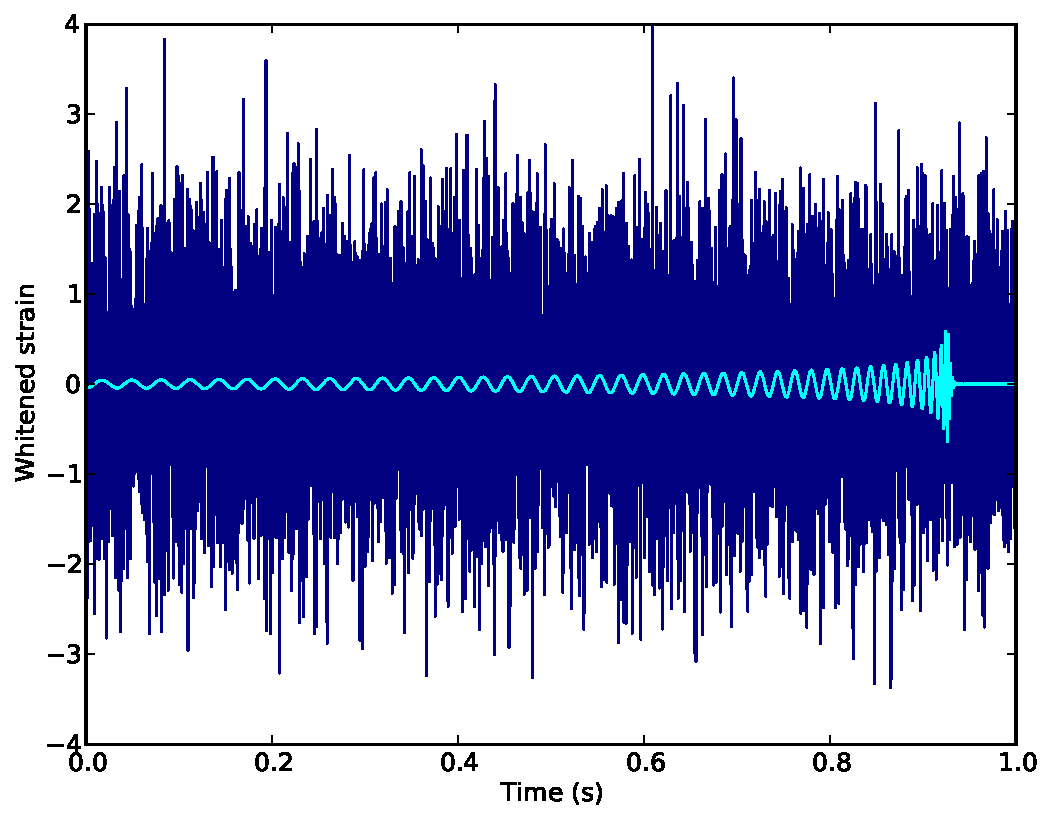
\includegraphics[width=\columnwidth]{figures/waveform.pdf}
\caption[Whitened noise-free timeseries of a \ac{BBH} signal]{A whitened noise-free timeseries of a \ac{BBH} signal sampled at $8192$~Hz with component masses $m_{1}=41.86\mathrm{M}_{\odot}$ and $m_{2}=6.65\mathrm{M}_{\odot}$ with optimal \ac{SNR} $\optsnr=8$ (cyan). The dark blue timeseries shows the same gravitational-wave signal with additive whitened Gaussian noise of unit variance. This latter timeseries is representative of the datasets used to train, validate, and test the deep neural network.\label{fig:waveform}}
\end{figure}

%
% define the CNN structure 
% 
\section{The Deep Network Approach}
%
% introduce convolutional neural networks
%
In our model, we use a variant of a deep learning algorithm called a 
\ac{CNN}~\cite{726791} composed of multiple layers (See Ch.~\ref{ch:chap_2}). 
The input layer holds the raw pixel values of the sample image which, in our 
case, is a 1-dimensional timeseries vector. The weight and bias 
parameters of the network are also in 1-dimensional vector 
form. This is opposed to the traditional 2-dimensional vector form more 
commonly used by \ac{ML} practitioners when applying \ac{CNN}s towards 
2-dimensional image analysis. We do not use a 2-dimensional 
vector form because our inputs are 1-dimensional, thus we would ideally 
like our \ac{CNN} filters to reflect that reality. Each neuron in 
the convolutional layer computes the convolution between the neuron's 
weight vector and the outputs from the layer below it, and then the 
result is summed with the bias vector. Neuron weight vectors are 
updated through an optimisation algorithm 
called back-propogation~\cite{LeCun1998}. Activation 
functions apply an element-wise non-linear operation 
rescaling their inputs onto a specific range and leaving the 
size of the previous layer's output unchanged. Pooling layers 
perform a downsampling operation along the spatial dimensions 
of their input. Finally we have a hidden layer connected to an output layer which
computes the inferred class probabilities. These values are 
input to a loss function, chosen as the 
binary cross-entropy~\cite{tensorflow2015-whitepaper}, defined as
%
% define the loss function
%
\begin{equation} \label{eq:loss} 
f(p,t) =
-\sum_{i\in\text{S}}t_{i}^{\mathrm{S}}\mathrm{log}(p^{\text{S}}_{i})-\sum_{i\in\text{N}}t_{i}^{\mathrm{N}}\mathrm{log}(p^{\text{N}}_{i}), 
\end{equation}
%
where $p^{\text{S/N}}_{i}$ is the predicted probability of the class signal+noise (S) or noise-only (N) and $t^{\text{S/N}}_{i}$ is the true value 
for the $i$'th training sample. The loss function is minimised when input data samples are assigned the correct class with the highest confidence. 

%
% describe the network choices that we have
%
In order to optimise a network, multiple hyper-parameters must be tuned. 
We define hyper-parameters as parameters that we are free to 
choose. Such parameters include the number and type of network layers, 
the number of neurons within each layer, the size of the neuron 
weight vectors, the max-pooling parameters, the type of activation 
functions, the preprocessing of input data, the learning rate, and the 
application (or otherwise) of specific deep learning techniques. We 
begin the process with the simplest network that provides a 
discernible level of effective classification. In most 
cases this consists of an input, convolutional, hidden, and 
logistic output layer. The optimal network structure was 
determined through multiple tests and tunings of hyperparameters by 
means of trial and error~\footnote{We have also used multiple other 
hyperparameter optimisation techniques, as introduced in Ch.~\ref{ch:chap_2}, 
in subsequent projects. We tried some of these optimisation schemes 
in Ch.~\ref{ch:chap_4}, but in the end settled on a network design which 
was determined through random trial and error.}.

%
% go into more detail about what we tried in network design
%
Within our optimisation process we experimented with rescaling the input 
data, which we found to have minimal effect on the network performance. The 
reason for this is that our input data is whitened and our 
signals are buried beneath the noise. Therefore our data is effectively 
prescaled on a range $\pm\mathcal{O}(1)$ due to the natural 
variation of Gaussian noise. We also experimented with using 
transfer learning~\cite{5288526} where networks pre-trained on 
high \ac{SNR} datasets are used as starting points for application to 
successively lower \ac{SNR} datasets. We found that there were no 
performance benefits in using this approach compared to training the 
network solely on each \ac{SNR} dataset separately. The network depth was 
adjusted between 2 and 10 convolutional layers. The inclusion of 
dropout (See Sec.~\ref{sec:ml_regularization} of Ch.~\ref{ch:chap_2})
was used within the final 2 hidden layers as a form of 
regularisation to avoid overfitting.

%
% describe how the training itself works to optimise the weights and biases
%
During the training stage an optimisation function (back-propagation) works 
by computing the gradient of the loss function (Eq.~\ref{eq:loss}) with 
respect to the weights of the network for a given training sample, 
then attempting to minimize 
that loss function. The value of the loss is propagated back 
through the network by taking the partial derivative of the loss with respect 
to the weights of the network and applying the chain rule. 
Using the calculated partial 
derivatives, one can then update the weight and bias terms of the network such 
that the loss is minimised.  Back propagation is done over multiple 
iterations where at each iteration the gradients are computed all at once over 
a batch of training samples. We also use Nesterov momentum~\cite{dozat2016incorporating}, which is described by  
%
\begin{equation} \label{eq:nesterov1}
v_{i} = \mu v_{i-1} - \eta \nabla f(\theta_{i-1} + \mu v_{i-1}),
\end{equation}
%
\begin{equation} \label{eq:nesterov2}
\theta_{i} = \theta_{i-1} + v_{i},
\end{equation} \\
%
where $\theta_{i-1}$ are the parameters of the neural network from the 
previous layer, $\theta_{i}$ are the parameters of the current layer 
of the network, $v_{i}$ is the momentum for the current layer, 
$\mu$ is a scalar constant term which determines 
the amount of momentum to apply per gradient update 
(the higher the number, the more momentum), $v_{i-1}$ is the 
momentum term from the previous layer, $\eta$ is the 
learning rate, $\nabla f(\theta_{i-1} + \mu v_{i-1})$ is the 
gradient of the model parameters with respect to the previous 
layer (including the momentum term from the previous layer ($\mu v_{i-1}$)).
There are a variety of 
initialisation schemes for the momentum term in each layer, but prior to 
training, the momentum in each layer is nominally simplified initially 
chosen from a uniform distribution between 0 and 1.
We use a learning rate of $\eta = 0.002$, and the Adam
optimiser~\cite{2014arXiv1412.6980K} 
which is parameterised by a set of user-defined hyperparameters given as: 
$\beta_{1}=0.9$, $\beta_{2}=0.999$, $\epsilon = 10^{-8}$ and a momentum
schedule of $0.004$ (See~\cite{2014arXiv1412.6980K} for 
further details on the function of 
these Adam hyperparameter values). We outline 
the structure of the final neural network architecture 
in Table~\ref{table:network}. We also note that the same 
network structure was used for each \ac{SNR}, but that a separate neural 
network was trained for every \ac{SNR} value.

%
% the CNN ranking statistic
%
The final ranking statistic that we extract from the \ac{CNN} analysis is 
taken from the output layer, composed of 2 neurons, where each neuron 
gives the inferred probability that the input data belongs to the 
noise or signal+noise class respectively. Both neurons
will produce a probability value between 0 and 1 with their sum 
being unity, which is the default behaviour of the 
softmax activation function given by 
%
\begin{equation}
    \mathrm{Softmax(x_i)} = \frac{e^{x_i}}{\sum_j e^{x_j}},
\end{equation}
%
where $e^{x_i}$ is the exponent of the value of one of the 2 output layer 
neurons for class $i$ and 
$\sum_j e^{x_j}$ is a summation over the exponent of both neuron 
output layer values, representing the predictions for all classes. 
The computational time spent on training the network for 
each SNR is $\mathcal{O}(1)$ hour on a single GPU. This one-time 
cost can be compared to the $\mathcal{O}(1 s)$ spent applying the 
trained network to all $25,000$ 1 s test data samples also 
using a single GPU. Therefore at the point of data taking this 
particular analysis can be run at ~$10^{4}$ times faster than real-time.

%
% Reference the loss, dp, lr  figure
%
In Fig.~\ref{fig:loss_curve}, we plot three different quantities 
as a function of training epoch for one of our networks trained 
on \ac{SNR} 8 signals. The top panel shows the loss as a 
function of training epoch, which we see decreases rapidly 
initially and then levels out as training progresses. In the 
middle panel, we show the detection probability (fraction of \ac{GW} 
signals correctly identified by the neural network) as a 
function of training epoch where the training, validation and testing 
detection probability are denoted as the purple, blue and orange curves 
respectively. The goal is to minimize the loss 
function, which will in turn maximise the detection probability of the 
classifier. We see in Fig.~\ref{fig:loss_curve} that as the loss decreases, 
the detection probability increases, indicating the the network is 
performing more accurately as training progresses. We should note here though 
that it does appear that the network is slightly overfitting to the 
training data. This is because the validation/testing detection probability 
curves (blue, orange) are lower than the training probability curve (purple). 
The bottom panel 
shows the learning rate used as a function of training epoch which 
oscillates between $10^{-3}$ and $5 \times 10^{-3}$. 

%
% Small discussion on cyclic learning rate
%
Our learning rate oscilates between a minimum and upper bound because 
we decided to employ a cyclic learning rate
scheduler~\cite{2015arXiv150601186S}. A cyclic learning rate is 
commonly used avoid saddle points, or local minima, in the 
loss function parameter space. Specifically, a learning rate which 
is too low will only apply small updates to the neural network weights and 
thus may get stuck in that saddle point. A cyclic learning rate 
will allow both large and small network weight updates to occur, thus 
increasing the likelihood of breaking out of saddle points. There is 
also the issue of choosing a poor initial learning rate at the beginning 
of training. If our network and/or optimiser is strongly influenced 
by the initial learning rate, we may never see the loss function 
minimised. A cyclic learning rate allows us apply a variety of learning 
rate values over a broad range, thus minimising the chance of choosing 
an inappropriate learning rate.

\begin{figure} 
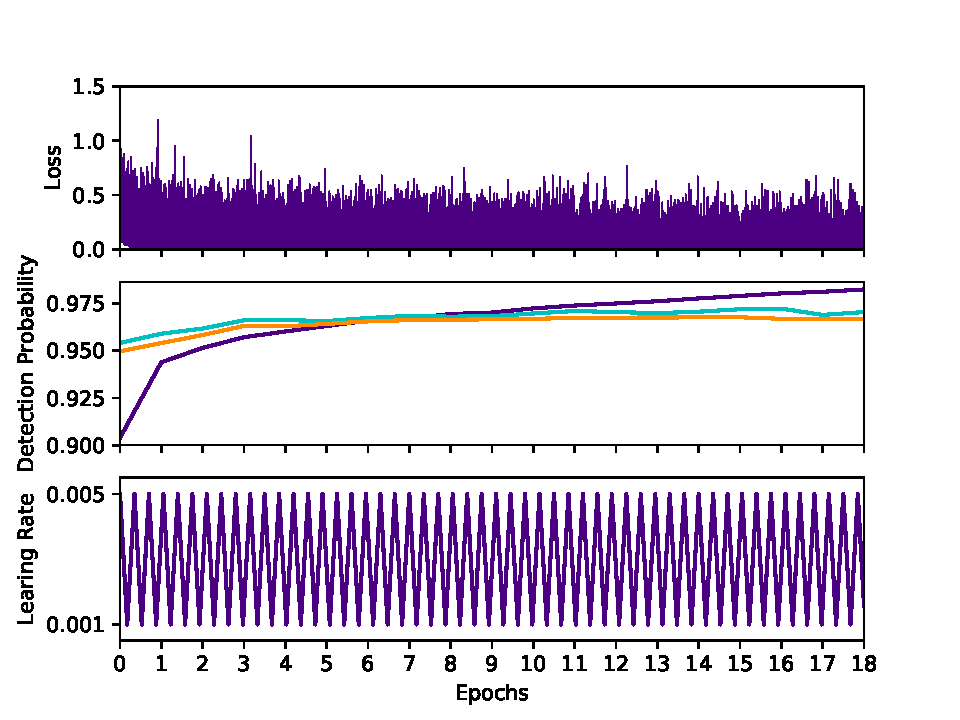
\includegraphics[width=\columnwidth]{figures/matching_matched_filtering_loss.pdf}
\caption[CNN loss, detection probability and learning rate plots illustrate 
how the network's performance is defined as a function of the number of 
training epochs.]{\label{fig:loss_curve} The loss, detection 
probability and learning rate plots (shown above top panel) for 
a network trained on \ac{SNR} 8 signals 
illustrate how the network's performance is defined as a function 
of the number of training epochs. The first initial epochs see an 
exponential decrease in the loss function and then a slowly falling 
values to follow. This indicates that the longer our network is trained, 
a limit with respect to the accuracy is approached. In our case, we 
cyclically adjust the learning rate to oscillate between 
$5 \times 10^{-4}$ and $10^{-3}$ at a constant frequency. The 
detection probability on training samples is represented by 
the purple curve, validation detection probability as the 
blue, and testing detection probability as the orange 
curve.}
\end{figure}

\begin{table}[]
\centering
\begin{tabular}{lccccccccc}
\hline
\hline
Parameter & \multicolumn{9}{c}{Layer}\\
\cline{2-10}
(Option) & 1 & 2 & 3 & 4 & 5 & 6 & 7 & 8 & 9 \\
\hline
Type & C & C & C & C & C & C & H & H & H \\
No. Neurons  & 8  & 8  & 16 & 16 & 32 & 32 & 64  & 64  & 2  \\
Filter Size  & 64 & 32 & 32 & 16 & 16  & 16  & n/a & n/a & n/a  \\
MaxPool Size & n/a & 8 & n/a & 6 & n/a & 4 & n/a & n/a & n/a \\
Drop out  & 0 & 0 & 0 & 0 & 0 & 0 & 0.5 & 0.5 & 0 \\
Act. Func. & Elu & Elu & Elu & Elu & Elu & Elu & Elu & Elu & SMax \\
\hline
\end{tabular}
\caption[CNN optimised network configuration consisting of 6 convolutional layers (C), followed by 3 hidden layers (H).]{The optimised network consisting of 6 convolutional layers (C), followed by 3 hidden layers (H). Max-pooling is performed on the first, fifth, and eighth layer, whereas dropout is only performed on the two hidden layers. Each layer uses an exponential linear unit (Elu) activation function (with range $[-1,\infty]$) while the last layer uses a Softmax (SMax) activation function in order to normalize the output values to be between zero and one so as to give a probability value for each class.\label{table:network}}
\end{table}

%
% define the matched-filter analysis
%
\section{Applying Matched-Filtering}
%
% introduce matched-filtering
%
In order to establish the power of the deep learning approach we must compare 
our results to the standard matched-filtering process used in the 
detection of \ac{CBC} signals~\cite{PhysRevD.85.122006,2013PhRvD..87b4033B}. 
The ranking statistic used in this case is the matched-filter 
\ac{SNR} numerically maximized over arrival time and analytically 
maximised over phase and distance~\cite{Anderson2011}. 
\hunter{Add reference back to chapter 1 if I add in the 
time, phase and amplitude matched filter maximisation derivation.}
By first defining the noise 
weighted inner product as a function of a time shift $\Delta t$ between 
$a$ and $b$ given as,
%
% define the matched-filtering SNR
%
\begin{equation}\label{eq:inner}
(a\mid b)(\Delta t) =
4\int_{f_{\mathrm{min}}}^{\infty}\frac{\tilde{a}(f)\tilde{b}^{*}(f)}{S_{\mathrm{n}}(f)}e^{2\pi i
f\Delta t}\,df,
\end{equation}
%
we can construct the squared matched-filter \ac{SNR} as 
%
\begin{equation}\label{eq:match_filt_snr_squared}
\rho^{2}(\Delta t)=\frac{(s\mid h)^{2}(\Delta t) + 
i(s\mid h)^{2}(\Delta t)}{(h\mid h)}
\end{equation}
%
where $s$ is the data containing noise and a potential signal, and $h$ 
is the noise-free gravitational-wave template and 
$\Delta t = 1/f_{s}$ and $f_s$ is the sampling
frequency~\cite{0264-9381-23-18-002}. 
For a given template this quantity is efficiently computed using the 
\ac{FFT}, where the \ac{FFT} allows the \ac{SNR} to be computed 
for all possible signal arrival times within the observation window with 
cost $N\log{N}$, where $N$ is the number of samples we have~\footnote{
If we didn't use the \ac{FFT}, then the brute force cost would $N^2$ (
correlating the template once costs $N$ operations and then shifting it by one 
bin and doing it again $N$ times.}. The maximum 
\ac{SNR} value from the output \ac{SNR} timeseries, defined by 
Eq.~\ref{eq:match_filt_snr_squared}, is also computed. The subsequent 
step is to further numerically maximize this quantity over a 
collection of component mass combinations. In this analysis a 
comprehensive template bank is generated in the $m_{1},m_{2}$ mass 
space covering our predefined range of masses. We use a 
maximum mismatch of $3\%$ and a lower frequency cutoff of 
$20~\mathrm{Hz}$ using the PyCBC geometric non-spinning template 
bank generation tool~\cite{pycbc-software,0264-9381-33-21-215004}. 
This template bank contained $8056$ individual templates. 

%
% describe the process of what we apply this to
%
When generating an \ac{SNR} timeseries (Eq.~\ref{eq:match_filt_snr_squared}) 
for an input dataset we select $f_{\mathrm{min}}$ according to the 
conservative case in which the signal merger occurs at the 0.95 
fraction of the 1~s timeseries. We therefore select only maximised 
\ac{SNR} timeseries values recovered from within the $[0.75,0.95]$ 
fractional range since this is the parameter space on which the 
\ac{CNN} has been trained. For the practical computation of the 
matched-filtering analysis we take each of the data samples from the 
testing dataset to compute the matched-filter ranking statistic.

%
% Describe the main results of the study
%

%
% a description of the main results
%
\section{Matching Matched Filtering Results}
%
% main introduction to results
%
After tuning the multiple hyper-parameters (Table~\ref{table:network}) 
and training the neural network (Fig.~\ref{fig:loss_curve}), we present 
the results of our \ac{CNN} classifier on a noise versus signal+noise 
sample set. With values of ranking statistics now assigned to each 
test data sample from both the \ac{CNN} and matched-filtering 
approaches, and having knowledge of the true class associated with 
each sample, we may now construct \ac{ROC} curves to compare performance. 

%
% introduce the confusion matrix results
%
A standard method for displaying the accuracy of a classifier is 
through a confusion matrix in which the number of samples of each 
true class identified as every possible class are listed in a 
square matrix. A fully diagonal matrix would imply no incorrectly 
classified samples and a uniform matrix would 
imply no classification power (with the 
stipulation that there are equal numbers of testing samples 
in each class). Classification, within the context of a confusion 
matrix, is defined as when the neural network predicts a value 
of greater than $p=0.5$ for a single class. We also highlight that this 
can't be done with the matched filtering approach and thus only 
show results from the \ac{CNN} in the confusion matrix. In
Fig.~\ref{fig:confusion} we show results for the \ac{CNN} approach 
from which we highlight the overall accuracy 
(the ratio of incorrectly identified samples to the total number of 
samples) is $[51.88\%,65.51\%,85.63\%,96.66\%,99.41\%,99.99\%]$ 
at $\rho_{\mathrm{opt}}=[2,4,6,8,10,12]$, for a fixed detection 
threshold of $p=0.5$. 
We highlight that the measure of \ac{CNN} accuracy 
illustrated by Fig.~\ref{fig:confusion} is 
interesting in general, but not useful for 
us in practice since we want to maximise the true alarm at a fixed 
false alarm value.

%
% confusion matrix plot
%
\begin{figure}[]
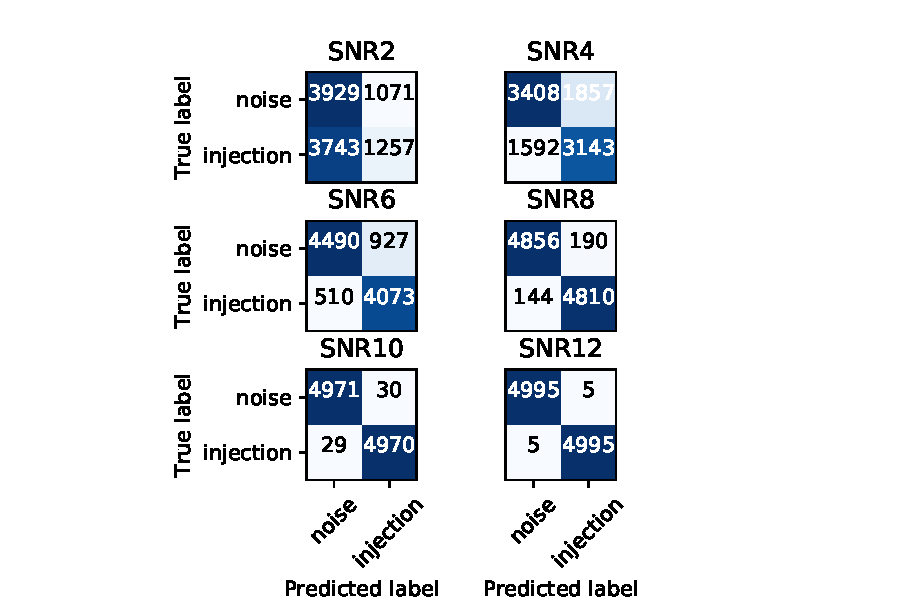
\includegraphics[width=\columnwidth] {figures/confusion_matrix.pdf}
\caption[Confusion matrices for testing datasets containing signals with 
optimal SNR $\rho_{\mathrm{opt}}=2,4,6,8,10,12$]{Confusion matrices for 
testing datasets containing signals with optimal \ac{SNR}
(Given in Eq.~\ref{eq:snr}) $\rho_{\mathrm{opt}}=2,4,6,8,10,12$. 
Numerical values superimposed within matrix elements represent the number of 
samples that were of true class indicated by the $y$-axis label but 
identified as the corresponding $x$-axis label. For our 2 class 
system these are equivalent to the numbers of true alarm, true dismissal, 
false dismissal, or false alarm, for a fixed detection threshold 
of $p=0.5$. The accuracy
percentages for all injection SNR values are listed as follows: $51.86\%$ at
$\rho_{\mathrm{opt}}=2$, $65.51\%$ at $\rho_{\mathrm{opt}}=4$, 
$85.63\%$ at $\rho_{\mathrm{opt}}=6$, $96.66\%$ at
$\rho_{\mathrm{opt}}=8$, $99.41\%$ at $\rho_{\mathrm{opt}}=10$ and $99.99\%$ at
$\rho_{\mathrm{opt}}=12$.\label{fig:confusion}}
\end{figure}

%
% describe ROC curves
%
In Fig.~\ref{fig:ROC_curves} we compare our \ac{CNN} results to that 
of matched-filtering. Given the ranking statistic from a particular 
analysis and defining a parametric threshold value on that statistic 
we are able to plot the fraction of noise samples incorrectly 
identified as signals (\ac{FAP}) versus the fraction of signal 
samples correctly identified (\ac{TAP}). These curves are defined 
as \ac{ROC} curves and a ranking statistic is deemed superior to 
another if at a given \ac{FAP} it achieves a higher detection 
probability. Our results show that the \ac{CNN} approach closely 
matches the sensitivity of matched-filtering for all test 
datasets across the range of \ac{FAP}s explored in this 
analysis\footnote{We are limited to a minimal \ac{FAP} of 
$\sim 10^{-4}$ due to the limited number of 
testing samples used.}. 
%It is not surprising to see that the 
%matched-filtering method using the optimal template consistently 
%performs better than both the nominal match-filtering method and 
%our deep learning classifier~\chris{NO. we don't show the optimal template result anywhere. Maybe we did at one point in the past. Either add those results to the figures or remove this reference.}. However, what is considerable is the comparison between the nominal~\chris{drop this "nominal" business if you are also going to drop the "optinal" template analysis.} matched-filtering and the deep learning classifier detection probability curves. 
It can clearly be seen that our classifier also exceeds the 
performance of the matched-filtering method at optimal 
\ac{SNR} $\rho_{\mathrm{opt}}=2,4,6$. This is an interesting result 
and is not entirely unexpected given that matched-filtering is not 
expected to be completely
optimal~\cite{2008arXiv0804.1161S,2021arXiv210403961Y}.

%
% show ROC curves
%
\begin{figure}[]
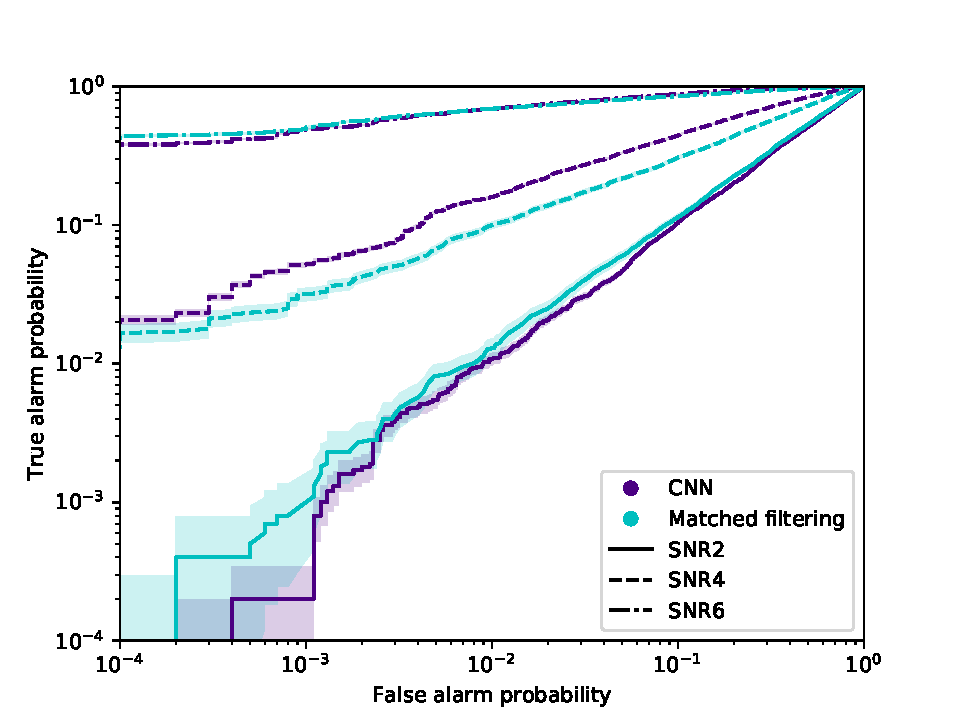
\includegraphics[width=\columnwidth] {figures/ROC_curves.pdf}
\caption[Receiver operating characteristic curves for test datasets containing signals with optimal signal to noise ratio, $\rho_{\mathrm{opt}}=2,4,6$]{The \ac{ROC} curves for test datasets containing signals with optimal \ac{SNR}, $\rho_{\mathrm{opt}}=2,4,6$. We plot the true alarm probability versus the false alarm probability estimated from the output of the \ac{CNN} (purple) and matched-filtering (cyan) approaches. Uncertainties in the true alarm probability correspond to 1-$\sigma$ bounds assuming a binomial distribution.} \label{fig:ROC_curves} 
\end{figure}

%
% finally discuss the efficiency plot
%
We can make an additional direct comparison between approaches by fixing a 
\ac{FAP} and plotting the corresponding \ac{TAP} versus the optimal 
\ac{SNR} of the signals in each test dataset. We show these efficiency 
curves in Fig.~\ref{fig:efficiency_curve} at \ac{FAP}s 
$10^{-1},10^{-2},10^{-3}$ for both the \ac{CNN} and matched-filtering 
approaches. We again see very good agreement between the approaches at all 
\ac{FAP}s with the \ac{CNN} sensitivity exceeding that of the 
matched-filter approach at low \ac{SNR} and high \ac{FAP}. 
Conversely we see the matched-filter sensitivity marginally exceeds 
the \ac{CNN} at high \ac{SNR} and low false alarm probability. 
This latter discrepancy could be mitigated by increasing the number 
of training samples in the CNN approach.

%
% show efficiency curve
%
\begin{figure}[]
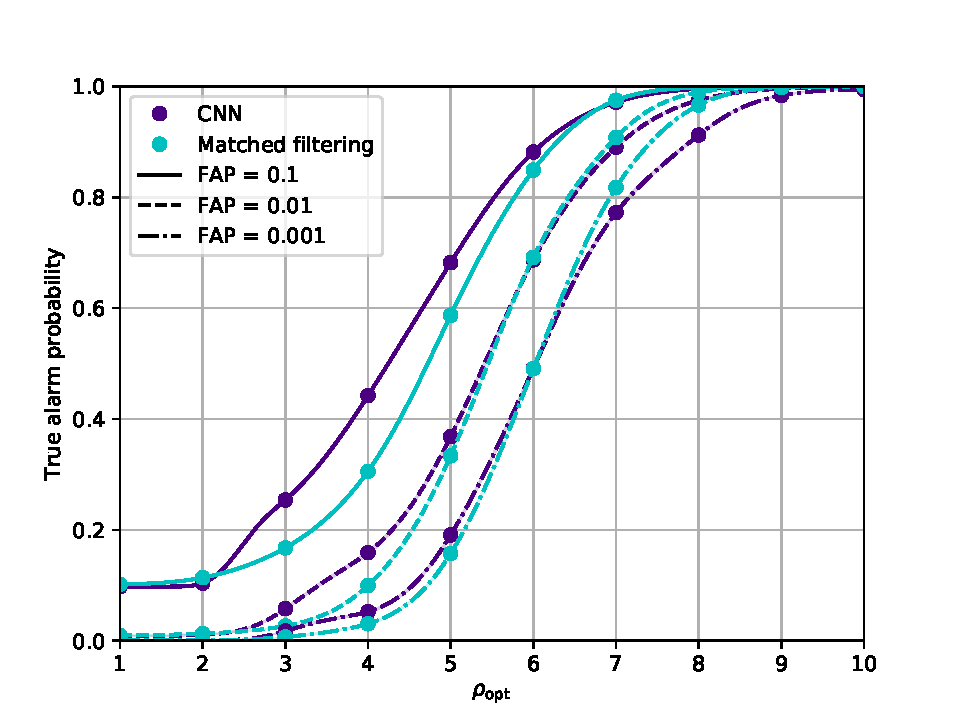
\includegraphics[width=\columnwidth] {figures/efficiency.pdf}
\caption[Efficiency curves comparing the performance of the CNNs~\chris{use acronym package - or maybe it doesn't work with short figure titles, BTW this short figure title isn't very short} and matched-filtering approaches for false alarm probabilities $10^{-1}$ (solid), $10^{-2}$ (dashed), $10^{-3}$ (dot-dashed).]{Efficiency curves comparing the performance of the \ac{CNN} and matched-filtering approaches for false alarm probabilities $10^{-1}$ (solid), $10^{-2}$ (dashed), and $10^{-3}$ (dot-dashed). The true alarm probability is plotted as a function of the optimal \ac{SNR} for the \ac{CNN} (purple) and the
matched-filtering (cyan) analyses. Solid dots indicate at which \ac{SNR} values analyses were performed and light shaded areas are representative of 
the statistical uncertainties in the curves (which are all smaller than the 
line thicknesses).\label{fig:efficiency_curve}} 
\end{figure}

%
% Summarise what you did, note key equations and specific results. If there is
% a main numerical result, quote it here. Then go back and make sure the
% abstract contains the most important results. Say what’s next
%
\section{Matching Matched Filtering Conclusions}\label{sec:mmf_conclusions} 
%
% summary of what we did
%
We have demonstrated that deep learning, when applied to \ac{GW}
timeseries data, is able to closely reproduce the results of a 
matched-filtering analysis in Gaussian noise. We employ a 
deep convolutional neural network with rigorously tuned 
hyperparameters and produce an output that returns a ranking 
statistic interpreted as the inferred probability that data contains a 
signal. Matched-filtering analyses are often described as 
the optimal approach for signal detection in Gaussian 
noise, but in reality are only close to
optimal~\cite{2008arXiv0804.1161S,2021arXiv210403961Y}. By building a 
neural network that is capable of matching the efficiency of matched 
filtering we answer a fundamental question regarding the applicability 
of neural networks for \ac{GW} data analysis. 

%
% Non Gaussian noise
%
In practice, searches for transient signals in \ac{GW} data are strongly 
affected by non-Gaussian noise artefacts. To account for this, 
standard matched-filtering approaches are modified to include 
carefully chosen changes to the ranking
statistic~\cite{PhysRevD.71.062001,0004-637X-849-2-118} together with 
the excision of poor quality data~\cite{1710.02185, 0264-9381-33-13-134001}. 
Our analysis represents a starting point from which a deep network 
can be trained on realistic non-Gaussian data. Since the 
claim of matched-filtering near optimality is applicable only in the 
Gaussian noise case, there exists the potential for deep networks 
to exceed the sensitivity of existing matched-filtering 
approaches in real data.

%
% On the use of multiple networks
%
We should also note that one of the downsides of our 
approach has been the use of separate 
neural networks for each \ac{SNR} value. This could easily 
be overcome by simply training a single \ac{CNN} model using a training set 
which contains \ac{GW} waveforms with multiple \ac{SNR} values. In fact, 
it was shown in~\cite{PhysRevD.100.044009} that single networks can generalise 
well to different \ac{SNR} values. 

%
% Other sources and final statement
%
In this work we have presented results for \ac{BBH} mergers, however, 
this method could be applied to other merger types, such as 
\ac{BNS} (as was shown in~\cite{PhysRevD.102.063015,KRASTEV2020135330}) 
and \ac{NSBH} signals. 
This supervised learning approach can 
also be extended to other well modelled \ac{GW} targets such as the 
continuous emission from rapidly rotating non-axisymmetric \ac{NS}s (as 
was done by~\cite{PhysRevD.100.044009}). Moreover, unsupervised 
approaches have the potential to be powerful detection tools in 
searches for unmodelled burst-like \ac{GW} signals, where it was 
shown in~\cite{2021CQGra..38o5005M} that \acp{GAN} could be 
used for such a task. Finally we 
mention the possibilities for parameter estimation~\cite{GEORGE201864}
~\hunter{More point estimate citations} where 
in the simplest cases an output regression layer can return 
point estimates of parameter values. As was exemplified in the 
case of GW170817~\cite{PhysRevLett.119.161101}, rapid detection confidence 
coupled with robust and equally rapid parameter estimates is 
critical for \ac{GW} multi-messenger astronomy. 

%
% Concluding remarks and transition
%
Since the publication of this paper, a lot has changed in the field of 
\ac{ML} for \ac{GW} astronomy. Many of the outstanding problems we outlined 
here in the conclusions have now been largely solved, such as applying 
deep learning towards other signal types~\cite{KRASTEV2020135330,PhysRevD.102.063015,2021CQGra..38o5005M,2021arXiv210513664B,Cuoco_2020}.\hunter{Need to finish this paragraph.}
In the following chapter 
(Ch.~\ref{ch:chap_5}) we will show how we have used \acp{CVAE} for the purpose 
of generating rapid Bayesian posterior parameter estimates which is 
consistent with other traditional sampling techniques. 

\chris{OK, obviously a very nice chapter. The things to be careful about in addition to my specific comments are the elements in the introduction and conclusion of this chapter that are now out of date. You *could* simply keep them as they are as a historical record of the time. However, that might not fly with your examiners. I would recommend updating these sections to just make sure that you aren't saying completely incorrect things or if you are referring to things that could be dne in the future when they have now actually been done, e.g., the CW stuff you talk about at the very end.}

\chris{Regarding showing any other results. ONLY if you could do things easily, I would be interested in the interpretibility aspects of this chapter. Could you make plots of filters and or layer outputs? It might prove insightful?}

\chris{Additionally, the stand out aspect of this work is how far we've advanced since we wrote it. You make the statement (and a referee might pick up on this) that there is lots of work still to be done on this topic. It begs the question "why didn't we do it?". Rather than actually doing more analysis for this chapter I think that you should add something in the conclusions (a paragraph or 2) about what has happened since this paper was published with regards to CBC detection using ML. You also want to use the final paragraph to segway into the topic of the next chapter on the more challenging topic of PE.}

%\chapter{Technical matching matched filtering}

\chapter{Variational Inference for GW Parameter Estimation}

%
% Introductory paragraph describing the content of the letter
%
% This format begins with a title of, at most, 15 words, followed by an
% introductory paragraph (not abstract) of approximately 150 words, summarizing
% the background, rationale, main results (introduced by "Here we show" or some
% equivalent phrase) and implications of the study. This paragraph should be
% referenced, as in Nature style, and should be considered part of the main
% text, so that any subsequent introductory material avoids too much redundancy
% with the introductory paragraph.
%
 
%
% background
%

\section{Introduction}

This is a cut and paste of our soon-to-be published paper (with appropriate modifications to format). Please see the following reference for our paper\cite{1909.06296}.

\ac{GW} detection is now
commonplace~\cite{PhysRevX.6.041015,PhysRevLett.119.161101} and as the
sensitivity of the global network of \ac{GW} detectors improves, we will
observe $\mathcal{O}(100)$s of transient \ac{GW} events per
year~\cite{2018LRR....21....3A}. The current methods used to estimate their
source parameters employ optimally sensitive~\cite{2009CQGra..26o5017S} but
computationally costly Bayesian inference approaches~\cite{1409.7215} where
typical analyses have taken between 6 hours and 5 days~\cite{gracedb_O3}.
%
% rationale
%
For \ac{BNS} and \ac{NSBH} systems prompt counterpart \ac{EM} signatures are
expected on timescales of 1 second -- 1 minute and the current fastest method
for alerting \ac{EM} follow-up observers~\cite{2016PhRvD..93b4013S}, can
provide estimates in $\mathcal{O}(1)$ minute, on a limited range of key source
parameters. 
%
% results
%
Here we show that a \ac{CVAE}~\cite{1904.06264,1812.04405} pre-trained on
\ac{BBH} signals can return Bayesian posterior probability estimates. The
training procedure need only be performed once for a given prior parameter
space and the resulting trained machine can then generate samples describing
the posterior distribution $\sim 6$ orders of magnitude faster than existing
techniques.
%
% currently ~240 words - needs cutting to ~150 approx 9.6 words per line

%%%%%%%%%%%%%%%%%%%%%%%%%%%%%%%%%%%%%%%%%%%%%%%%%%%%%%%%%%%%%%%%%%%%%%
% INTRODUCTION
%%%%%%%%%%%%%%%%%%%%%%%%%%%%%%%%%%%%%%%%%%%%%%%%%%%%%%%%%%%%%%%%%%%%%%
%
% introduction - this section has to expand upon what has mentioned in the
% abstract background (which was only ~50 words). It needs to cover the state of
% the gravitational wave field and the number of detections expected in the next
% ~5 years. It should briefly discuss the issue of low latency EM follow up. It
% needs to cover Bayesian inference (not in too much detail) and the signal model
% we are interested in here (again, not too much detail but enough for the
% average Nature reader). It then needs to introduce machine learning and focus
% mainly on how our scheme works. We also need to include a statement about how
% the training data priors affect the result (are they really the priors?)
%
% Intro to the detection era with the LVC
%
%With the overwhelmingly successful observation runs of O1 and O2 now complete,
%\ac{LIGO} and Virgo have produced a large catalogue of \ac{GW} data covering
%both \ac{BBH} and \ac{BNS} signals~\cite{1811.12907}. Over the next five years
%we expect the number of detections to increase to be upwards of $\sim180$
%\ac{BNS} and $\sim400$ BBH events per year~\cite{1304.0670,1811.12907}. This
%large influx in the number of detections will put an increased amount of
%pressure on the current \ac{GW} inference methods used for parameter
%estimation.  

%
% From GW detection, to parameter estimation
%
The problem of detecting \acp{GW} has largely been solved through the use of
template based matched-filtering, a process recently replicated using machine
learning techniques~\cite{GEORGE201864,PhysRevLett.120.141103,GebKilParHarSch}.
Once a \ac{GW} has been identified through this process, Bayesian inference,
known to be the optimal approach~\cite{2009CQGra..26o5017S}, is used to extract
information about the source parameters of the detected \ac{GW} signal.

%
% Set up parameter estimation problem
%
In the standard Bayesian \ac{GW} inference approach, we assume a signal and
noise model and both may have unknown parameters that we are either interested
in inferring or prefer to marginalise away. Each parameter is given a prior
astrophysically motivated probability distribution and in the \ac{GW} case, we
typically assume a Gaussian additive noise model (in reality, the data is not
truly Gaussian). Given a noisy \ac{GW} waveform, we would like to find an
optimal procedure for inferring some set of the unknown \ac{GW} parameters.
Such a procedure should be able to give us an accurate estimate of the
parameters of our observed signal, whilst accounting for the uncertainty
arising from the noise in the data.

%
% Describe Bayes Theorem
%
According to Bayes' Theorem, a posterior probability distribution on a set of
parameters, conditional on the measured data, can be represented as
%
\begin{align}\label{eq:bayes_theorem} 
p(x|y) &\propto p(y|x) p(x), 
\end{align}
%
where $x$ are the parameters, $y$ is the observed data, $p(x|y)$ is the
posterior, $p(y|x)$ is the likelihood, and $p(x)$ is the prior on the
parameters. The constant of proportionality, which we omit here, is
$p(y)$, the probability of our data, known as the Bayesian evidence or the
marginal likelihood. We typically ignore $p(y)$ since it is a constant and for
parameter estimation purposes we are only interested in the shape of the
posterior.

%
% brief statement on the sampling algorithms
%
Due to the size of the parameter space typically encountered in \ac{GW}
parameter estimation and the volume of data analysed, we must stochastically
sample the parameter space in order to estimate the posterior.  Sampling is
done using a variety of techniques including Nested
Sampling~\cite{skilling2006,cpnest,dynesty} and Markov chain Monte Carlo
methods~\cite{emcee,ptemcee}. The primary software tools used by the \ac{LIGO}
parameter estimation analysis are \texttt{LALInference} and
\texttt{Bilby}~\cite{1409.7215,1811.02042}, which offer multiple sampling
methods.  
  
%
% Intro to machine learning section
%
Machine learning has featured prominently in many areas of \ac{GW} research
over the last few years. These techniques have shown to be particularly
promising in signal
detection~\cite{GEORGE201864,PhysRevLett.120.141103,GebKilParHarSch}, glitch
classification~\cite{0264-9381-34-6-064003} and earthquake
prediction~\cite{Coughlin_2017}. We also highlight a recent development in
\ac{GW} parameter estimation (published in parallel and independent to this
work) where 1- and 2-dimensional marginalised Bayesian posteriors are produced
rapidly using neural networks~\cite{2019arXiv190905966C}. This is done without
the need to compute the likelihood or posterior during training which is also a
characteristic of the approach described in this letter.

%
% Introduce CVAEs
%
Recently, a type of neural network known as \ac{CVAE} was
shown to perform exceptionally well when applied towards computational imaging
inference~\cite{1904.06264,NIPS2015_5775}, text to image
inference~\cite{1512.00570}, high-resolution synthetic image
generation~\cite{1612.00005} and the fitting of incomplete heterogeneous
data~\cite{1807.03653}. It is this type of machine learning network that we
apply in the \ac{GW} case to accurately approximate the Bayesian posterior
$p(x|y)$. 

%
% Brief introduction to loss functions used in the neural networks
%
The construction of a \ac{CVAE} begins with the definition of a quantity to be
minimised (referred to as a cost function). We can relate that aim to
that of approximating the posterior distribution by minimising the cross
entropy, defined as
%
\begin{align}\label{eq:cross_ent} 
H(p,r) &= -\int dx\, p(x|y) \log r_{\theta}(x|y) 
\end{align}
%
between the true posterior $p(x|y)$ and $r_{\theta}(x|y)$, the parametric
distribution that we will use neural networks to construct and which we aim to
be equal to the true posterior. In this case $\theta$ represents a set of
trainable neural network parameters. Starting from this point it is possible to
derive a computable form for the cross-entropy that is reliant on a set of
unknown functions that can be modelled by variational encoder
and decoder neural networks. The details of the derivation are described in
the methods section and in~\cite{1904.06264}. The final form of the
cross-entropy loss function is given by the bound
%
\begin{align}\label{eq:cost3}
H \lesssim -\frac{1}{N}\sum_{n=1}^{N}&\Big[\log
r_{\theta_{2}}(x_{n}|z_{n},y_{n})\nonumber\\
&-\text{KL}\left[q_{\phi}(z|x_{n},y_{n})||r_{\theta_{1}}(z|y_{n})\right]\Big],
\end{align}
%
and requires three fully-connected networks; two encoder networks (labelled
$\textrm{E}_1$, $\textrm{E}_2$ in Fig.~\ref{fig:network_config}) representing
the functions $r_{\theta_{1}}(z|y)$ and $q_{\phi}(z|x,y)$ respectively, and one
decoder network (D) representing the function $r_{\theta_{2}}(x|z,y)$. The
function $\text{KL}(\cdot||\cdot)$ denotes the \ac{KL} divergence and
the variable $z$ represents locations within the \emph{latent space}.  This
latter object is typically a lower dimensional space within which the encoder
networks attempt to represent their input data. In practice, during the
training procedure the various integrations that are part of the derivation are
approximated by a sum over a batch of $N$ training data samples (indexed by $n$
above) at each stage of training. Training is performed via a series of steps
detailed in the methods section.

\begin{figure}
    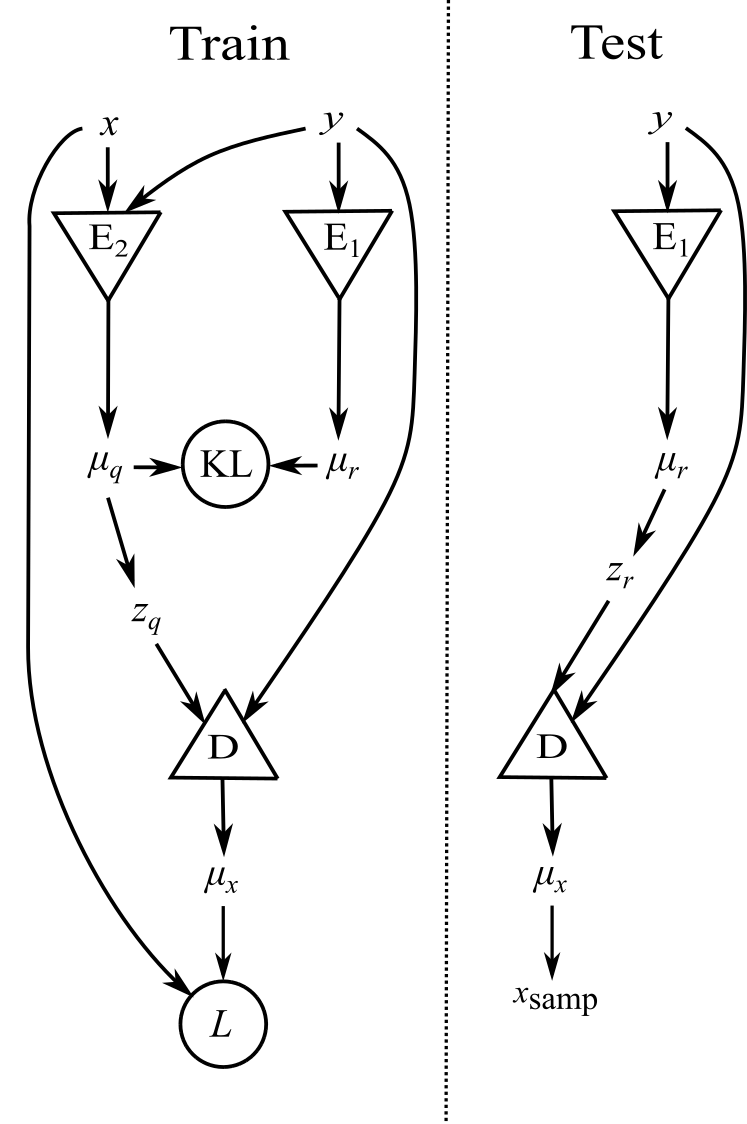
\includegraphics[width=\columnwidth]{network_setup.png}
    \caption{\label{fig:network_config} The configuration of the \ac{CVAE}
neural network. During training (left-hand side), a training set of noisy
\ac{GW} signals ($y$) and their corresponding true parameters ($x$) are given
as input to encoder network $\textrm{E}_2$, while only $y$ is given to
$\textrm{E}_1$.  The K-L divergence (Eq.~\ref{eq:kl}) is computed between the
encoder output latent space representations (defined by $\mu_q$ and $\mu_r$)
forming one component of the total cost function.  Samples ($z_q$) from the
$\text{E}_{2}$ latent space representation are generated and passed to the
decoder network D together with the original input data $y$. The output of the
decoder ($\mu_x$) describes a distribution in the physical space and the
\ac{ELBO} cost component $L$ is computed by evaluating that distribution at the
value of the original input $x$. When performed in batches this scheme allows
the computation of the total cost function Eq.~\ref{eq:cost3}. After having
trained the network, we test (right-hand side) using only the $\textrm{E}_1$
encoder and the decoder D to produce samples ($x_{\text{samp}}$) from the
posterior $p(x|y)$.}
\end{figure}

%
% word count ~1500 - approx 9 words per line
%

%%%%%%%%%%%%%%%%%%%%%%%%%%%%%%%%%%%%%%%%%%%%%%%%%%%%%%%%%%%%%%%%%%%%%%
% RESULTS
%%%%%%%%%%%%%%%%%%%%%%%%%%%%%%%%%%%%%%%%%%%%%%%%%%%%%%%%%%%%%%%%%%%%%%
%
% results - here you would outline the process of comparison between the
% standard approach and the new one. Define training and test data and how Bilby
% is run on all test data for comparison. How do we then train our network. How
% do we then produce results on the test data. Here you refer to results plots
% but try to not make conclusion statements (just descriptive). Also include the
% speed analysis here.
%
%
% Intro to the results - what are we trying to do?
%
\section{Results}
We present results on $256$ single detector \ac{GW} test \ac{BBH} waveforms in
simulated advanced detector noise~\cite{aligo_noisecurves} and compare between
variants of the existing Bayesian approaches and the \ac{CVAE}. Posteriors
produced by the \texttt{Bilby} inference library~\cite{1811.02042} are used as
a benchmark in order to assess the efficiency and quality of our machine
learning approach with the existing method for posterior sampling.

%
% describe the Bilby analysis 
%
For the benchmark analysis we assume that 5 parameters are unknown: the
component masses $m_1,m_2$, the luminosity distance $d_{\text{L}}$, the time of
coalescence $t_{0}$, and the phase at coalescence $\phi_0$. For each
parameter we use a uniform prior with ranges and fixed values defined in
Table~\ref{tab:prior_ranges}.
%~\chris{we might want to
%change this to be a $d$-squared prior to demonstrate the application of priors
%in the \texttt{VItamin} training stage.} 
We use a sampling frequency of $256$~Hz, a timeseries duration of 1 second, and 
the waveform model used is \texttt{IMRPhenomPv2}~\cite{1809.10113} with a
minimum cutoff frequency of $20$Hz. For each input test waveform we run the
benchmark analysis using multiple sampling algorithms available within
\texttt{Bilby}. For each run and sampler we extract $3000$ samples from the
posterior on the 5 physical parameters.  

%
% the VItamin process
%
The \ac{CVAE} training process used as input $10^{6}$ waveforms corresponding
to parameters drawn from the same priors as assumed for the benchmark analysis.
The waveforms are also of identical duration, sampling frequency, and waveform
model as used in the benchmark analysis. When each waveform is placed within a
training batch it is given a unique detector noise realisation after which the
data is whitened using the same advanced detector
\ac{PSD}~\cite{aligo_noisecurves} from which the simulated noise is
generated\footnote{Although we whiten the data as input to our network the
whitening is simply to scale the input to a level more suitable to neural
networks and need not be performed with the true \ac{PSD}.}. The \ac{CVAE}
posterior results are produced by passing our $256$ whitened noisy testing set
of \ac{GW} waveforms as input into the testing path of the pre-trained
\ac{CVAE}~\ref{fig:network_config}. For each input waveform we sample until we
have generated $3000$ posterior samples on 4 physical parameters
($x=(m_1,m_2,d_{\text{L}},t_{0})$). We choose to output a subset of the full
5-dimensional space to demonstrate that parameters (such as $\phi_0$ in this
case) can (if desired) be marginalized out within the \ac{CVAE} procedure
itself, rather than after training. 

%
% 1-D overlap results
%
\begin{figure*}
    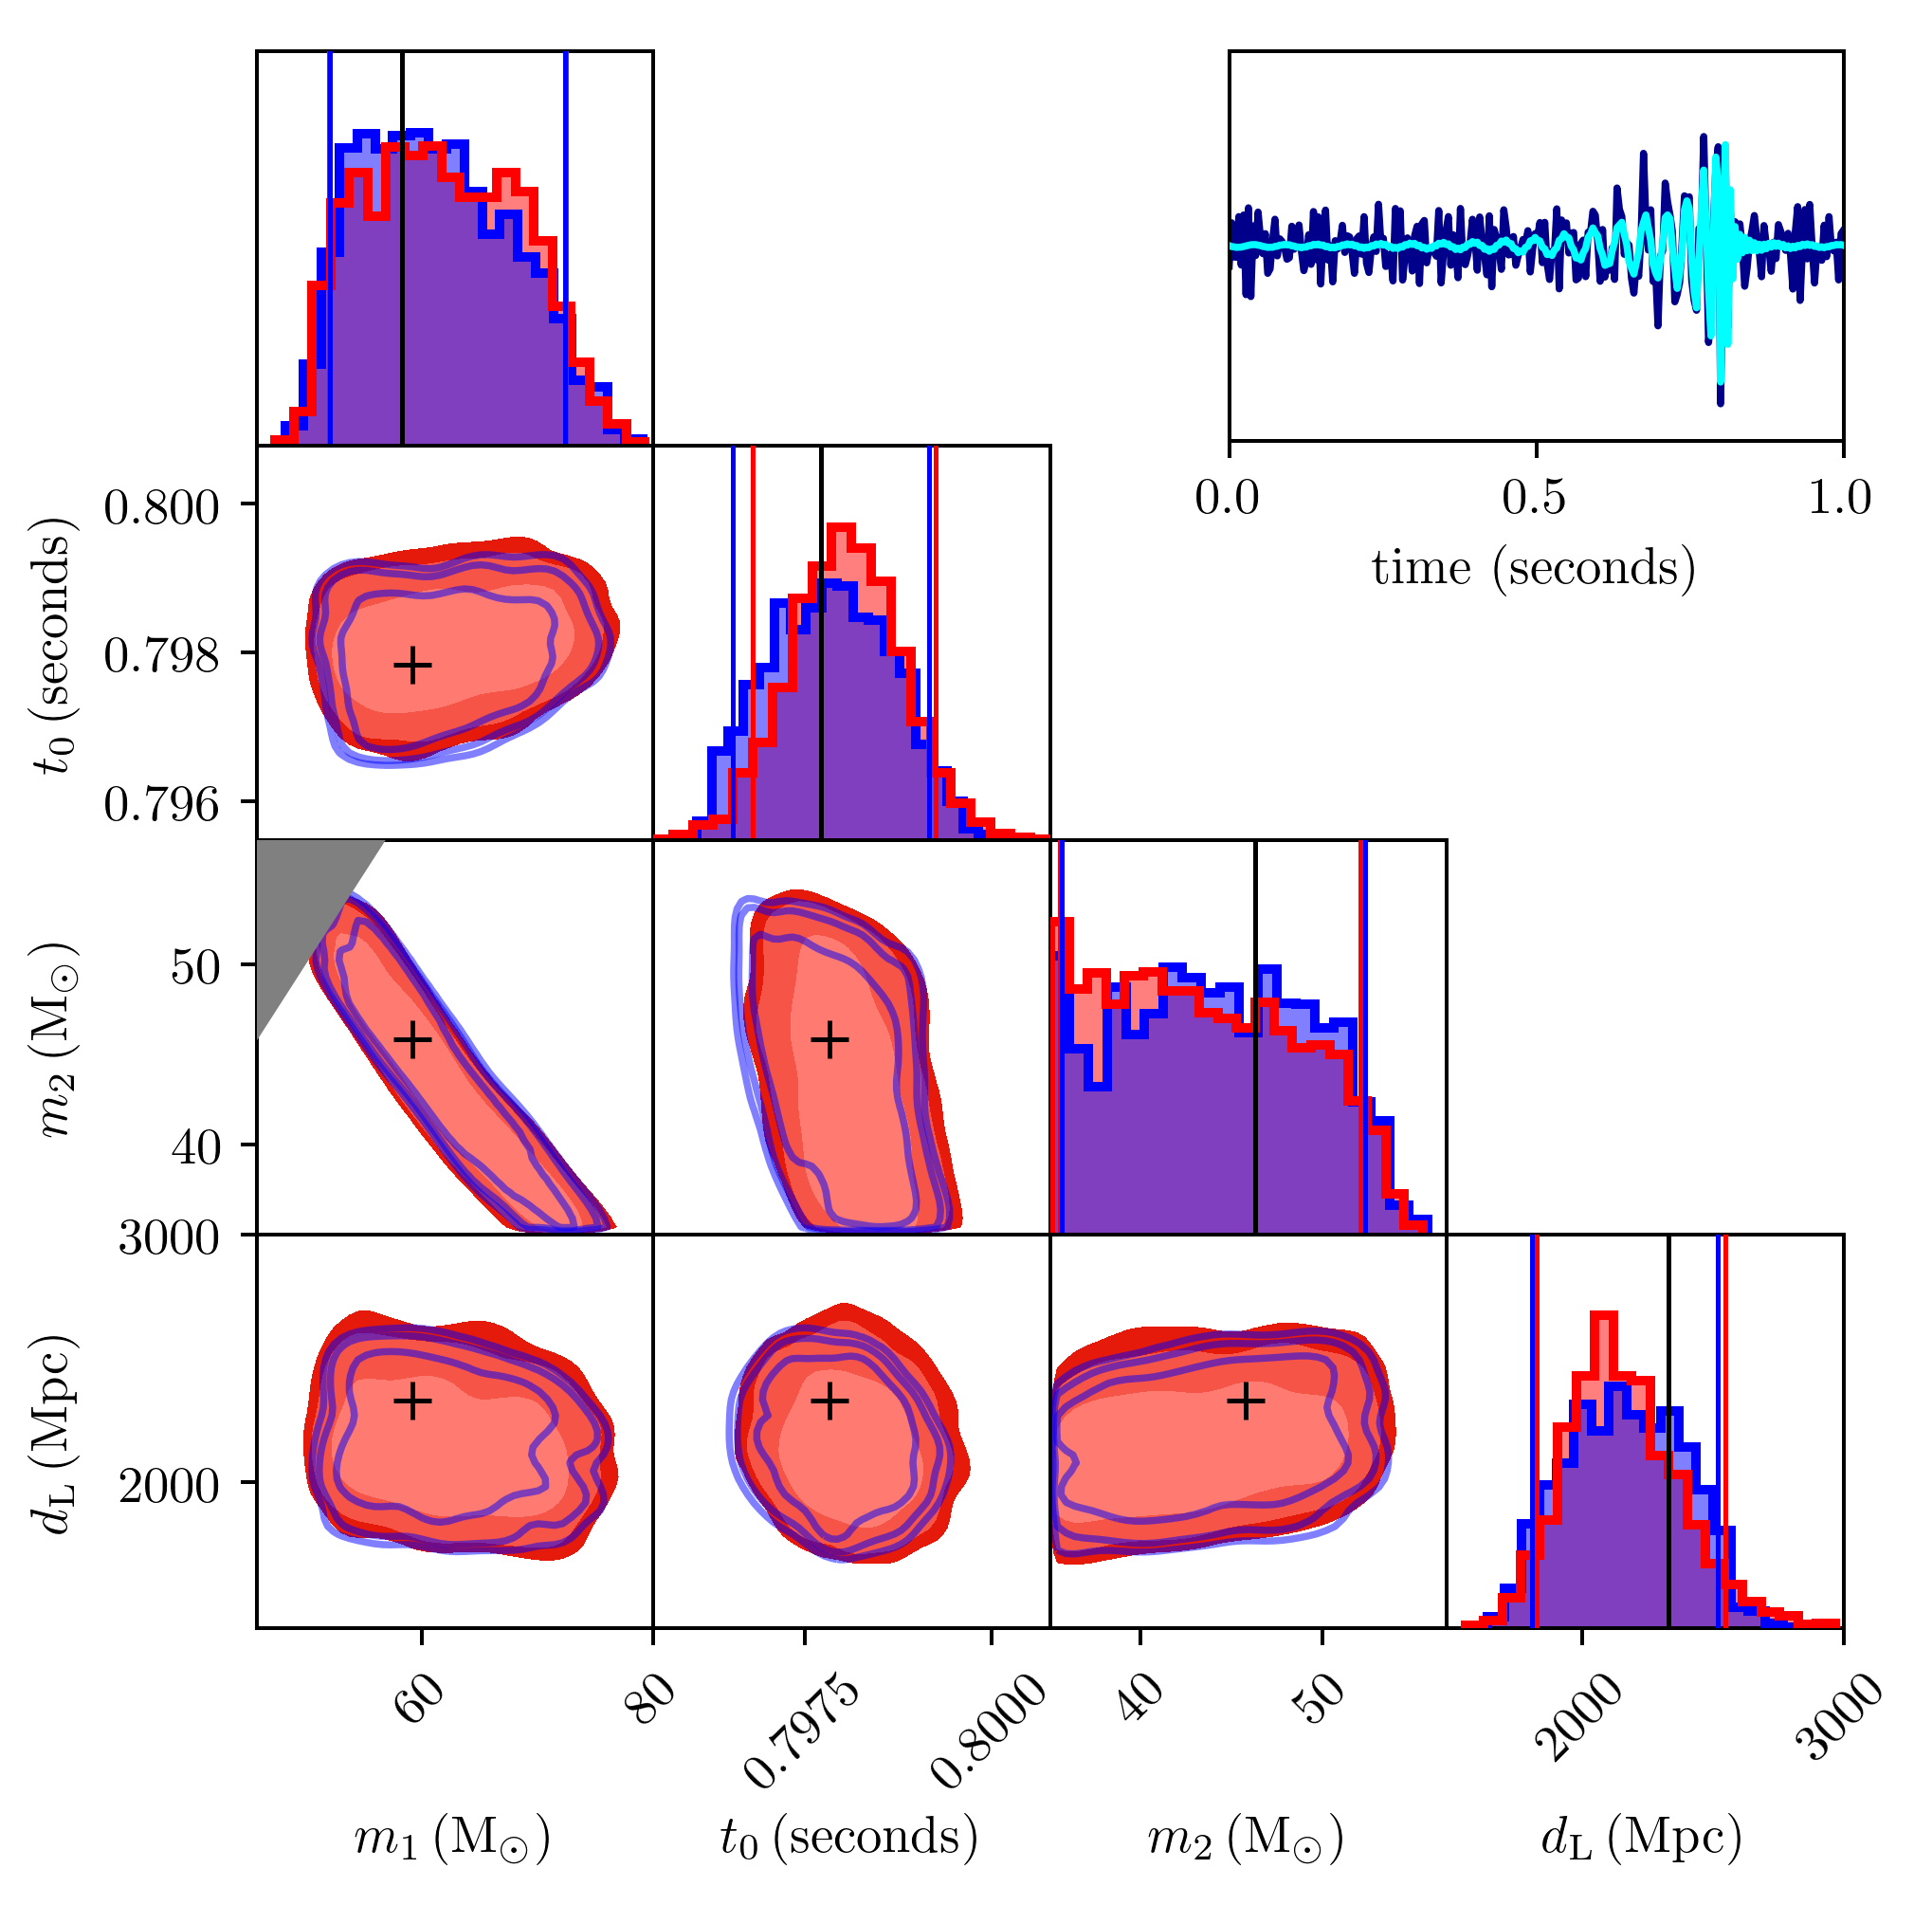
\includegraphics[width=\textwidth]{corner_testcase0.png}
    \caption{\label{fig:corner_plot} Corner plot showing 2 and 1-dimensional
marginalised posterior distributions for one example test dataset. Filled (red)
contours represent the posteriors obtained from the \ac{CVAE} approach and
solid (blue) contours are the posteriors output from our baseline analysis
(\texttt{Bilby} using the dynesty sampler). In each case, the contour boundaries
enclose $68,90$ and $95\%$ probability. One dimensional histograms of the
posterior distribution for each parameter from both methods are plotted along
the diagonal. Blue and red vertical lines represent the $5$---$95\%$ symmetric
confidence bounds for \texttt{Bilby} and variational inference respectively.
Black crosses and vertical black lines denote the true parameter values of the
simulated signal. The original whitened noisy timeseries $y$ and the noise-free
signal are plotted in blue and cyan respectively in the upper right hand
panel. The test signal was simulated with optimal signal-to-noise ratio of
13.9.}
\end{figure*}

%
% discuss the corner plot results
%
We can immediately illustrate the accuracy of our machine learning predictions
by directly plotting 2 and 1-dimensional marginalised posteriors generated
using the output samples from our \ac{CVAE} and \texttt{Bilby} approaches
superimposed on each other. We show this for one example test dataset in
Fig.~\ref{fig:corner_plot} where the strong agreement between both
\texttt{Bilby} (blue) and the \ac{CVAE} (red) is clear. 

%We provide additional test case example corner plots in the methods
%section. 
%\hunter{Add more corner plots in methods
%section}~\chris{Maybe, but more corner plots aren't going to convince people.
%We need to agregate the results into a single figure somehow (like the KL
%values). I think something based on the 1-D intervals would be nice.}

%
% mention the pp plot and KL distribution results
%
In Figs.~\ref{fig:pp_plot},\ref{fig:kl_results} (see the Methods section) we show
the results of 2 statistical tests (the \ac{PP} plot test and \ac{KL}
divergence tests) performed on the entire test dataset and between all
samplers. In both cases the tests indicate that the \texttt{VItamin} sampler
performs as well as any other sampler in comparison with the full set of
samplers.

%
% discuss the speed of the analysis
%
The dominating computational cost of running \texttt{VItamin} lies in the
training time, which can take of order several hours to complete. We stress
that once trained, there is no need to retrain the network unless the user
wishes to use different priors $p(x)$ or assume different noise
characteristics. The speed at which posterior samples are generated for all
samplers used, including \texttt{VItamin}, is shown in Table~\ref{Tab:speed}.
Run-time for the benchmark samplers is defined as the time to complete their
analyses when configured using their default parameters~\cite{1811.02042}. For
\texttt{VItamin} this time is defined as the total time to produce $3000$
samples. For our test case of \ac{BBH} signals \texttt{VItamin} produces
samples from the posterior at a rate which is $\sim 6$---$7$ orders of
magnitude faster than our benchmark analysis using current inference
techniques. 

%\chris{One more thing to add, especially if the other KL, AD, and PP plots
%aren't convincing, is a plot displaying 1D confidence bounds compared between
%bilby and VItamin. Imagine a plot with the x-axis as distance and the y-axis
%steps through test data with increasing true distance. for each test data you
%plot 2 error bars horizontally (one for bilby and one for VItamin) spanning the
%range of 90\% confidence. You would hopefully get nearly identical pairs of
%errorbars stacked vertically. Technically you could do this for all parameters
%(and you should) but we might only put one of the plots in the paper (if at
%all).}

%
% I feel the need, the need for speed, table
% 
\begin{table}
\centering
\caption{Durations required to produce samples from each of
the different posterior sampling approaches.}
\begin{tabular}[t]{lcccc}
\toprule
\multirow{2}{*}{sampler} & \multicolumn{3}{c}{run time (seconds)} & \multirow{2}{*}{ratio
$\displaystyle\frac{\tau_{\text{VItamin}}}{\tau_{X}}$} \\
& min & max & median & \\
\hline
Dynesty\footnote{The benchmark samplers all produced $\mathcal{O}(3000-
	10000)$ samples dependent on the default sampling parameters used.} & 602 & 1538 & 774\footnote{The reader may note that benchmark sampler run times are a few orders of magnitude lower than what is typical of a complete \ac{BBH} analysis ($\mathcal{O}(10^{4} -10^{5})$ seconds). This is primarily due our use of a reduced parameter space, low sampling rate and choice of sampler hyperparameters.} & $2.6\times 10^{-6}$ \\
Emcee & 2005 & 11927 & 4351 & $4.6\times 10^{-7}$ \\
Ptemcee & 3354 & 12771 & 4982 & $4.0\times 10^{-7}$ \\
Cpnest & 1431 & 5405 & 2287 & $8.8\times 10^{-7}$ \\
\texttt{VItamin}\footnote{For the \texttt{VItamin} sampler $3000$ samples are
produced as representative of a typical posterior. The run time is independent
of the signal content in the data and is therefore constant for all test cases.} & \multicolumn{3}{c}{\bm{$2\times 10^{-3}$}} & 1 \\
\botrule
\end{tabular}
\label{Tab:speed}
\end{table}

%
% word count ~960 - approx 9.6 words per line
%

%%%%%%%%%%%%%%%%%%%%%%%%%%%%%%%%%%%%%%%%%%%%%%%%%%%%%%%%%%%%%%%%%%%%%%
% CONCLUSIONS
%%%%%%%%%%%%%%%%%%%%%%%%%%%%%%%%%%%%%%%%%%%%%%%%%%%%%%%%%%%%%%%%%%%%%%
%
% conclusions - now draw conclusions about the quality of the comparison
% results. Highlight the current limitations but also highlight the importance of
% this for the GW field (multi-detector is easy, additional parameters are easy,
% longer datasets may be a challenge regarding GPU memory?, we don't have to
% assume a noise model if we inject training data into real noise, we do rely on
% well defined signal models, EM-follow up in very low latency, can we use
% transfer learning if we want to retrain, ...) End with broader statements about
% inference in other fields and how this is applicable across the sciences.
%
% recap and main result
%
\section{Conclusions}

In this letter we have demonstrated that we are able to reproduce, to a high
degree of accuracy, Bayesian posterior probability distributions generated
through machine learning. This is accomplished using \acp{CVAE} trained on
simulated \ac{GW} signals and does not require the input of precomputed
posterior estimates. We have demonstrated that our neural network model which,
when trained, can reproduce complete and accurate posterior estimates in
$\mathcal{O}(1)$ millisecond, can achieve the same quality of results as the
trusted benchmark analyses used within the LIGO-Virgo Collaboration.

%
% CBC implications and why this is a game-changer - speed for EM followup
%
The significance of our results is most evident in the orders of magnitude
increase in speed over existing approaches. Improved low-latency alerts will be
especially pertinent for signals from \ac{BNS} mergers (e.g.
GW170817~\cite{PhysRevLett.119.161101}) and \ac{NSBH} signals where parameter
estimation speed will no longer be limiting factor\footnote{The complete
low-latency pipeline includes a number of steps. The process of \ac{GW} data
acquisition is followed by the transfer of data. There is then the
corresponding analysis and the subsequent communication of results to the
\ac{EM} astronomy community after which there are physical aspects such as
slewing observing instruments to the correct pointing.} in observing the prompt
\ac{EM} emission expected on shorter time scales than is achievable with
existing \ac{LVC} analysis tools such as Bayestar~\cite{2016PhRvD..93b4013S}.

%
% CBC implications and why this is a game-changer - faster, modular
%
The predicted number of future detections of \ac{BNS} mergers ($\sim
180$~\cite{2018LRR....21....3A}) will severely strain the \ac{GW} community's
current computational resources using existing Bayesian methods. Future
iterations of our approach will provide full-parameter estimation on \ac{CBC}
signals in $<1$ second on a single \ac{GPU}. Our trained network is also
modular, and can be shared and used easily by any user to produce results. The
specific analysis described in the letter assumes a uniform prior on the signal
parameters. However, this is a choice and the network can be trained with any
prior the user demands, or users can cheaply resample accordingly from the
output of the network trained on the uniform prior. We also note that our
method will be invaluable for population studies since populations may now be
generated and analysed in a full-Bayesian manner on a vastly reduced time
scale. 

%
% future work, current limitations and prospects
%
For \ac{BBH} signals, \ac{GW} data is usually sampled at $1$---$4$ kHz
dependent upon the mass of binary. We have chosen to use the noticeably low
sampling rate of 256Hz and a single detector configuration largely in order to
decrease the computational time required to develop our approach. We do not
anticipate any problems in extending our analysis to higher sampling
frequencies other than an increase in training time and a larger burden on the
\ac{GPU} memory. Our lower sampling rate naturally limited the chosen \ac{BBH}
mass parameter space to high mass signals. We similarly do not anticipate that
extending the parameter space to lower masses will lead to problems but do
expect that a larger number of training samples may be required. Future work
will incorporate a multi-detector configuration at which point parameter
estimation will be extended to sky localisation. 

%
% Non gaussian noise and the final statement
%
In reality, \ac{GW} detectors are affected by non-Gaussian noise artefacts and
time-dependent variation in the detector noise \ac{PSD}. Existing methods
incorporate a parameterised \ac{PSD} estimation into their
inference~\cite{2015PhRvD..91h4034L}. To account for these within our scheme,
we would retrain our network at regular intervals using samples of real
detector noise (preferably recent examples to best reflect the state of the
detectors). Our work can naturally be extended to include the full range of
\ac{CBC} signal types but also to any and all other parameterised \ac{GW}
signals and to analyses of \ac{GW} data beyond that of ground based
experiments. Given the abundant benefits of this method, we hope that a variant
of this of approach will form the basis for future \ac{GW} parameter
estimation.
%
% word count ~620
%

%
% word count 80 
%


%% Here is the endmatter stuff: Supplementary Info, etc.
%% Use \item's to separate, default label is "Acknowledgements"

%%%%%%%%%%%%%%%%%%%%%%%%%%%%%%%%%%%%%%%%%%%%%%%%%%%%%%%%%%%%%%%%%%%%%%
% METHODS
%%%%%%%%%%%%%%%%%%%%%%%%%%%%%%%%%%%%%%%%%%%%%%%%%%%%%%%%%%%%%%%%%%%%%%
%
% methods - Everything that we couldn't fit in. Mostly validation plots.
%
\section{Methods}\label{sec:methods}
%
%Put methods in here.  If you are going to subsection it, use
%\verb|\subsection| commands.  Methods section should be less than
%800 words and if it is less than 200 words, it can be incorporated
%into the main text.

%
% What is an autoencoder?
%
Conditional variational autoencoders are a form of variational autoencoder
which are conditioned on an observation, where in our case the observation is a
1-dimensional \ac{GW} time series signal $y$. The autoencoders from which
variational autoencoders are derived are typically used for problems involving
image reconstruction and/or dimensionality reduction. They perform a regression
task whereby the autoencoder attempts to predict its own given input (model the
identity function) through a ``bottleneck layer'', a limited  and therefore distilled representation of
the input parameter space. An autoencoder is composed of two neural networks,
an encoder and a decoder~\cite{gallinari1987memoires}. %\cite{LIOU20083150}. 
The encoder network takes as
input a vector, where the number of dimensions is a fixed number predefined by
the user. The encoder converts the input vector into a (typically) lower
dimensional space, referred to as the {\it{latent space}}. A representation of
the data in the latent space is passed to the decoder network which generates a
reconstruction of the original input data to the encoder network. Through
training, the two sub-networks learn how to efficiently represent a dataset
within a lower dimensional latent space which will take on the most important
properties of the input training data. In this way, the data can be compressed
with little loss of fidelity. Additionally, the decoder simultaneously learns
to decode the latent space representation and reconstruct that data back to its
original form (the input data).

%
% What is a variational autoencoder?
%
The primary difference between a variational autoencoder~\cite{1812.04405} and
an autoencoder concerns the method by which locations within the latent space
are produced. In our variant of the variational autoencoder, the output of the
encoder is interpreted as a set of parameters governing statistical
distributions (in our case the means and variances of multivariate Gaussians).
In proceeding to the decoder network, samples from the latent space ($z$) are
randomly drawn from these distributions and fed into the decoder, therefore
adding an element of variation into the process. A particular input can then
have a range of possible outputs. In both the decoder and the encoder networks
we use fully-connected layers (although this is not a constraint and any
trainable network architecture may be used).

%%%%%%%%%%%%%%%%%%%%%%%%%%%%%%%%%%%%%%%%%%%%%%%%%%%%%%%%%%%%%%%%%%%%%%
\subsection{Cost function derivation}
%
% A description of the loss function derivation 
%
We will now derive the cost function and the corresponding network structure
and we begin with the statement defining the aim of the analysis. We wish to
obtain a function that reproduces the posterior distribution (the probability
of our physical parameters $x$ given some measured data $y$). The cross entropy
between 2 distributions is defined in Eq.~\ref{eq:cross_ent} where we have made
the distributions explicitly conditional on $y$ (our measurement). In this case
$p(x|y)$ is the target distribution (the true posterior) and $r_{\theta}(x|y)$
is the parametric distribution that we will use neural networks to construct.
The variable $\theta$ represents the trainable neural network parameters. 

The cross-entropy is minimised when $p(x|y)=r_{\theta}(x|y)$ and so by
minimising
%
\begin{align}\label{eq:cost1}
H &= -\text{E}_{p(y)}\left[\int dx\,p(x|y) \log r_{\theta}(x|y)\right],
\end{align}
% 
where $\text{E}_{p(y)}[\cdot]$ indicates the expectation value over the
distribution of measurements $y$, we therefore make the parametric distribution
as similar as possible to the target for all possible measurements $y$.

Converting the expectation value into an integral over $y$ weighted by $p(y)$
and applying Bayes' theorem we obtain
%
\begin{align}\label{eq:cost1}
H &= -\int dx\,p(x)\int dy\,p(y|x)\log r_{\theta}(x|y)
\end{align}
%
where $p(x)$ is the prior distribution on the physical parameters $x$.

The \ac{CVAE} network outlined in Fig.~\ref{fig:network_config} makes use of a
conditional latent variable model and our parametric model is constructed from
the product of 2 separate distributions marginalised over the latent space
%
\begin{align}\label{eq:latent_model}
r_{\theta}(x|y) &= \int dz\,r_{\theta_{1}}(z|y)r_{\theta_{2}}(x|z,y).
\end{align}
%  
We have used $\theta_{1}$ and $\theta_{2}$ to indicate that the 2 separate
networks modelling these distributions will be trained on these parameter sets
respectively. Both new conditional distributions are modelled as $n_{z}$
dimensional multivariate uncorrelated Gaussian distributions (governed by their
means and variances). However, this still allows $r_{\theta}(x|y)$ to take a
general form (although it does limit it to be unimodal).  

One could be forgiven in thinking that by setting up networks that simply aim
to minimise $H$ over the $\theta_{1}$ and $\theta_{2}$ would be enough to solve
this problem. However, as shown in~\cite{NIPS2015_5775} this is an intractable
problem and a network cannot be trained directly to do this. Instead we define
a recognition function $q_{\phi}(z|x,y)$ that will be used to derive an
\ac{ELBO}. Here we use $\phi$ to represent the trainable parameters of an
encoder network ($\text{E}_{2}$).

Let us first define the \ac{KL} divergence between 2 of our
distributions as
%
\begin{align}\label{eq:kl}
\text{KL}&\left[q_{\phi}(z|x,y)||r_{\theta_{2}}(z|x,y)\right] = \\
&\int dz\,q_{\phi}(z|x,y)
\log\left(\frac{q_{\phi}(z|x,y)}{r_{\theta_{2}}(z|x,y)}\right).\nonumber
\end{align}
%  
It can be shown, after some manipulation, that
%
\begin{align}\label{eq:elbo1}
\log r_{\theta}(x|y) &= L + \text{KL}\left[q_{\phi}(z|x,y)||r_{\theta_{?}}(z|x,y)\right],
\end{align}
%
where the \ac{ELBO} $L$ is given by
%
\begin{align}\label{eq:elbo2}
L &= \int dz\,
q_{\phi}(z|x,y)\log\left(\frac{r_{\theta_{2}}(x|z,y)r_{\theta_{1}}(z|y)}{q_{\phi}(z|x,y)}\right)
\end{align}
%
and is so-named since $\text{KL}$ cannot be negative and has a minimum of zero.
Therefore, if we were to find a $q_{\phi}(z|x,y)$ function (optimised on
$\phi$) that minimised the \ac{KL}-divergence then we can state that
%
\begin{align}
\log r_{\theta}(x|y) &\geq L.
\end{align}
%
After some further manipulation of Eq.~\ref{eq:elbo2} we find that
%
\begin{align}\label{eq:logr}
\log r_{\theta}(x|y) \geq  &\text{E}_{q_{\phi}(z|x,y)}\left[\log
r_{\theta_{2}}(x|z,y)\right] \nonumber\\
&-\text{KL}\left[q_{\phi}(z|x,y)||r_{\theta_{1}}(z|y)\right].
\end{align}
%
We can now substitute this inequality into Eq.~\ref{eq:cost1} (our cost
function) to obtain
%
\begin{align}\label{eq:cost2}
H \leq  -\int dx\, p(x)\int dy &\,p(y|x)
\Big[\text{E}_{q_{\phi}(z|x,y)}\left[\log r_{\theta_{2}}(x|z,y)\right]
\nonumber\\
&-\text{KL}\left[q_{\phi}(z|x,y)||r_{\theta_{1}}(z|y)\right]\Big],  
\end{align}
%
which can in practice be approximated as a stochastic integral over draws of
$x$ from the prior, $y$ from the likelihood function $p(y|x)$, and from the
recognition function, giving us Eq.~\ref{eq:cost3}, the actual function
evaluated within the training procedure.

%
% loss plot
%
\begin{figure}
    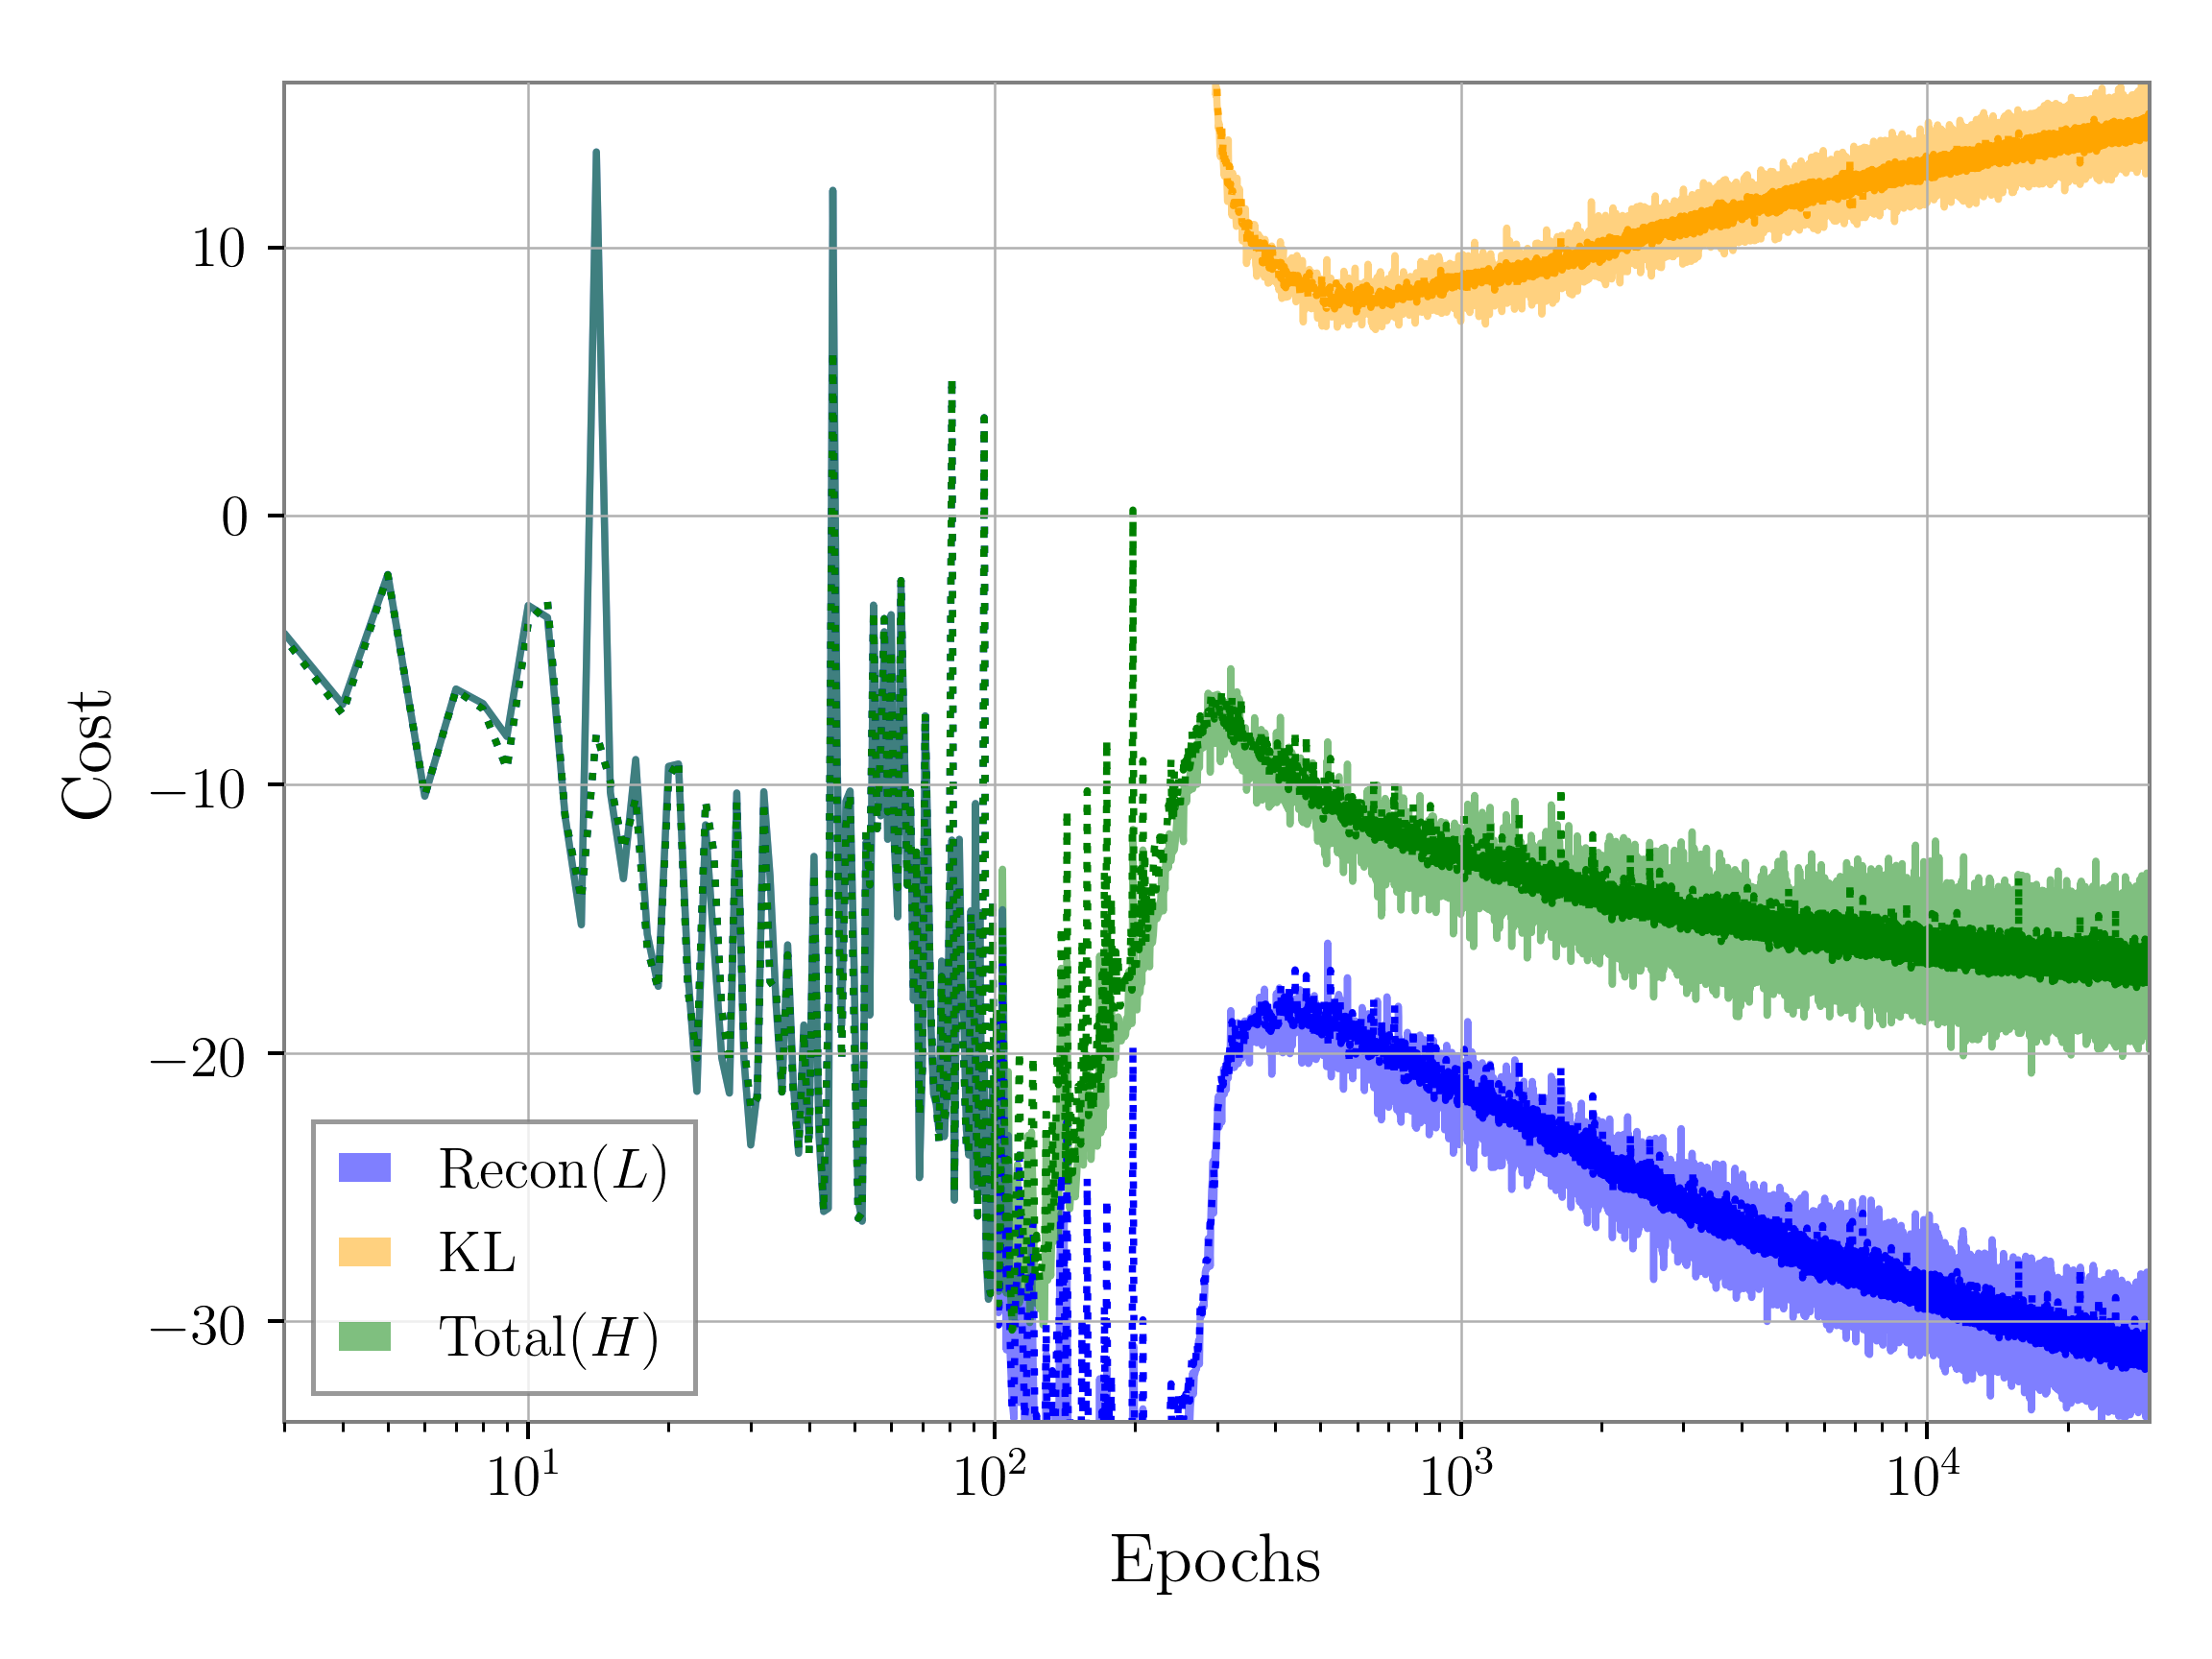
\includegraphics[width=\columnwidth]{inv_losses_log.png}
\caption{\label{fig:loss_log} The cost as a function of training iteration. We
show the \ac{ELBO} cost function component (blue), the \ac{KL} divergence
component (orange) and total cost (green). The total cost is simply a
summation of the 2 components and one training iteration is defined as
training over one batch of signals.}
\end{figure}

%
% Priors
%
\begin{table}
\centering
\caption{The uniform prior boundaries and fixed parameter values used on the \ac{BBH} signal parameters for the benchmark
and the \ac{CVAE} analyses.}
\begin{tabular}[t]{lcccc}
\toprule
Parameter name & symbol & min & max & units \\
\hline
mass 1 & $m_1$ & 35 & 80 & solar masses \\
mass 2 & $m_2$\footnote{Additionally $m_2$ is constrained such that
$m_{2}<m_{1}$.} & 35 & 80 & solar masses \\
luminosity distance & $d_{\text{L}}$ & 1 & 3 & Gpc \\
time of coalescence & $t_{0}$ & 0.65 & 0.85 & seconds \\
phase at coalescence & $\phi_{0}$ & 0 & $2\pi$ & radians \\
\hline
right ascension & $\alpha$ & \multicolumn{2}{c}{1.375} & radians \\
declination & $\delta$ & \multicolumn{2}{c}{-1.2108} & radians \\
inclination & $\iota$ & \multicolumn{2}{c}{0} & radians \\
polarisation & $\psi$ & \multicolumn{2}{c}{0} & radians \\
spins & - & \multicolumn{2}{c}{0} & - \\
epoch & - & \multicolumn{2}{c}{1126259642} & GPS time \\
detector & - & \multicolumn{2}{c}{LIGO Hanford} & - \\
\botrule
\end{tabular}
\label{tab:prior_ranges}
\end{table}

%%%%%%%%%%%%%%%%%%%%%%%%%%%%%%%%%%%%%%%%%%%%%%%%%%%%%%%%%%%%%%%%%%%%%%
\subsection{The training procedure}
%
% Introduce the training process
%
Having set up a cost function composed of 3 probability functions that have
well defined inputs and outputs where the mapping of those inputs to outputs is
governed by the parameter sets $\theta_{1},\theta_{2},\phi$. These parameters
are the weights and biases of 3 neural networks acting as (variational)
encoder, decoder, and encoder respectively. To train such a network one must
connect the inputs and outputs appropriately to compute the cost function $H$
and back-propagate cost function derivatives to update the network parameters.
The network structure shown schematically in Fig.~\ref{fig:network_config}
shows how for a batch of $N$ sets of $x$ and corresponding $y$ values, the cost
function is computed during each iteration of training. 

%
% Go through the training step by step
%
Training is performed via a series of steps illustrated in
Fig.~\ref{fig:network_config}.
%
\begin{itemize}
%
\item The encoder $\textrm{E}_1$ is given a set of training \ac{GW} signals
($y$) and encodes $y$ into a set of variables $\mu_q$ defining a distribution
in the latent space. In this case $\mu_q = (\mu_{q0},\sigma^{2}_{q})$ describes
the first 2 central moments (mean and variance) for each dimension of a
uncorrolated (diagonal covariance) multivariate Gaussian distribution.
%
\item The encoder $\textrm{E}_2$ takes a combination of both the data $y$ and
the true parameters $x$ defining the \ac{GW} signal and encodes this into
parameters defining another uncorrelated multivariate Gaussian distribution in
the same latent space. These parameters we denote by
$\mu_{r}=(\mu_{r0},\sigma^{2}_{r})$ again representing the means and variances.
%
\item We then sample from the distribution described by $\mu_{q}$ giving us
samples $z_{q}$ within the latent space.
%
\item These samples, along with their corresponding $y$ data, then go to the
decoder D which outputs $\mu_{x}=(\mu_{x0},\sigma^{2}_{q})$, a set of parameters (much like
$\mu_q,\mu_r$) that define the moments of an uncorrelated  multivariate Gaussian
distribution in the physical $x$ space.
 %
\item The first term of the loss function (Eq.~\ref{eq:cost3}) is then computed
by evaluating the probability density defined by $\mu_x$ at the true $x$
training values. The component of the loss allows the network to learn how to
predict accurate values of $x$ but to also learn the intrinsic variation due to
the noise properties of the data $y$. It is important to highlight that the
\ac{GW} parameter predictions from the decoder D do describe a multivariate
Gaussian, but as is shown in our results (see Fig.~\ref{fig:corner_plot}), this
does \emph{not} imply that our final output posterior estimates will also be
multivariate Gaussians.
%
\item Finally the loss component described by the \ac{KL} divergence between the
distributions described by $\mu^{q}$ and $\mu^{r}$ is computed using
%
\begin{align}\label{eq:klgauss}
\text{KL}&\left[q_{\phi}(z|x_{n},y_{n})||r_{\theta_{1}}(z|y_{n})\right] = \\
&\frac{1}{2}\sum_{j=1}^{n_{z}}\left[\frac{\sigma_{q,j}^{2}}{\sigma_{r,j}^{2}} +
\frac{(\mu_{r0,j}-\mu_{q0,j})^{2}}{\sigma_{r,j}^{2}}+
\log\left(\frac{\sigma_{r,j}^{2}}{\sigma_{q,j}^{2}}\right)\right] -
\frac{n_{z}}{2}.\nonumber 
\end{align}
%
Here we highlight that we do not desire that the network tries to make these 2
distributions equal to each other. Rather, we want the ensemble network to
minimise the total cost (of which this is a component).
%
\end{itemize}

%
% Some practical aspects of the training
%
As is standard practice in machine learning applications, the cost is computed
over a batch of training samples and repeated for a pre-defined number of
iterations. Completion of training is determined by comparing output posteriors
on test samples with those of \texttt{Bilby} iteratively during training. This
comparison is done using standard figures of merit such as the \ac{KL}
divergence and the P-P plot. We also assess training completion based on
whether the cost function and its component parts (Fig.~\ref{fig:loss_log})
have converged. We use a single Nvidia Tesla V100 \acp{GPU} with $16/32$ Gb of
RAM although consumer grade ``gaming" \ac{GPU} cards are equally fast for this
application.


%%%%%%%%%%%%%%%%%%%%%%%%%%%%%%%%%%%%%%%%%%%%%%%%%%%%%%%%%%%%%%%%%%%%%%
\subsection{Network and Training parameters}
%
% Describe the specific network hyper-parameters
%
For our purposes, we found that $\sim3\times10^6$ training iterations, a batch
size of $512$ training samples and a learning rate of $10^{-4}$ was sufficient.
We used a total of $10^6$ training samples in order to adequately cover the
\ac{BBH} parameter space. We additionally ensure that an (effectively) infinite
number of noise realizations are employed by making sure that every time a
training sample is used it is given a unique noise realisation despite only
having a finite number of waveforms. Each neural network ($\text{E}_1$,
$\text{E}_2$, D) is composed of 3 fully connected layers and has $2048$ neurons
in each layer with ReLU~\cite{nair2010rectified} activation functions between
layers. We use a latent space dimension of $8$ and we consider training
complete when both components to the loss function have converged to
approximately constant values or when comparisons with benchmark test
posteriors indicate no significant changes in the output posterior.

%%%%%%%%%%%%%%%%%%%%%%%%%%%%%%%%%%%%%%%%%%%%%%%%%%%%%%%%%%%%%%%%%%%%%%
\subsection{The testing procedure}
%~\chris{Hunter, note that we only need to
%do the first pass through E1 only once for a given piece of data do the real
%cost is only in the other steps. This will likely only change the timing by
%~25\% so it might not be worth doing the tests again. Just bear it in mind.}
%
%
% Introduce the testing procedure
%
After training has completed and we wish to use the network for inference we
follow the procedure described in the right hand panel of
Fig.~\ref{fig:network_config}. Given a new $y$ data sample (not taken from the
training set) we simply input this into the encoder $\textrm{E}_1$ from which we
obtain a single value of $\mu_{r}$ describing a distribution (conditional on the
data $y$) in the latent space. We then repeat the following steps:

%
% Go through the testing step by step
%
\begin{itemize}
%
\item We randomly draw a latent space sample $z_r$ from the latent space
distribution defined by $\mu_r$.
%
\item Our $z_r$ sample and the corresponding original $y$ data are fed as input to our
pre-trained decoder network (D). The decoder network returns a set of moments
$\mu_{x}$ which describe a multivariate Gaussian distribution in the physical
parameter space.
%
\item We then draw a random $x$ realisation from that distribution.
%
\end{itemize}
%

%
% Final testing thoughts
%
A comprehensive representation in the form of samples drawn from the entire joint
posterior distribution can then be obtained by simply repeating this procedure
with the same input data (see Eq.~\ref{eq:latent_model}).

%
% K-L divergence results
%
\subsection{Additional tests}
%
% P-P plot
%
\begin{figure}
    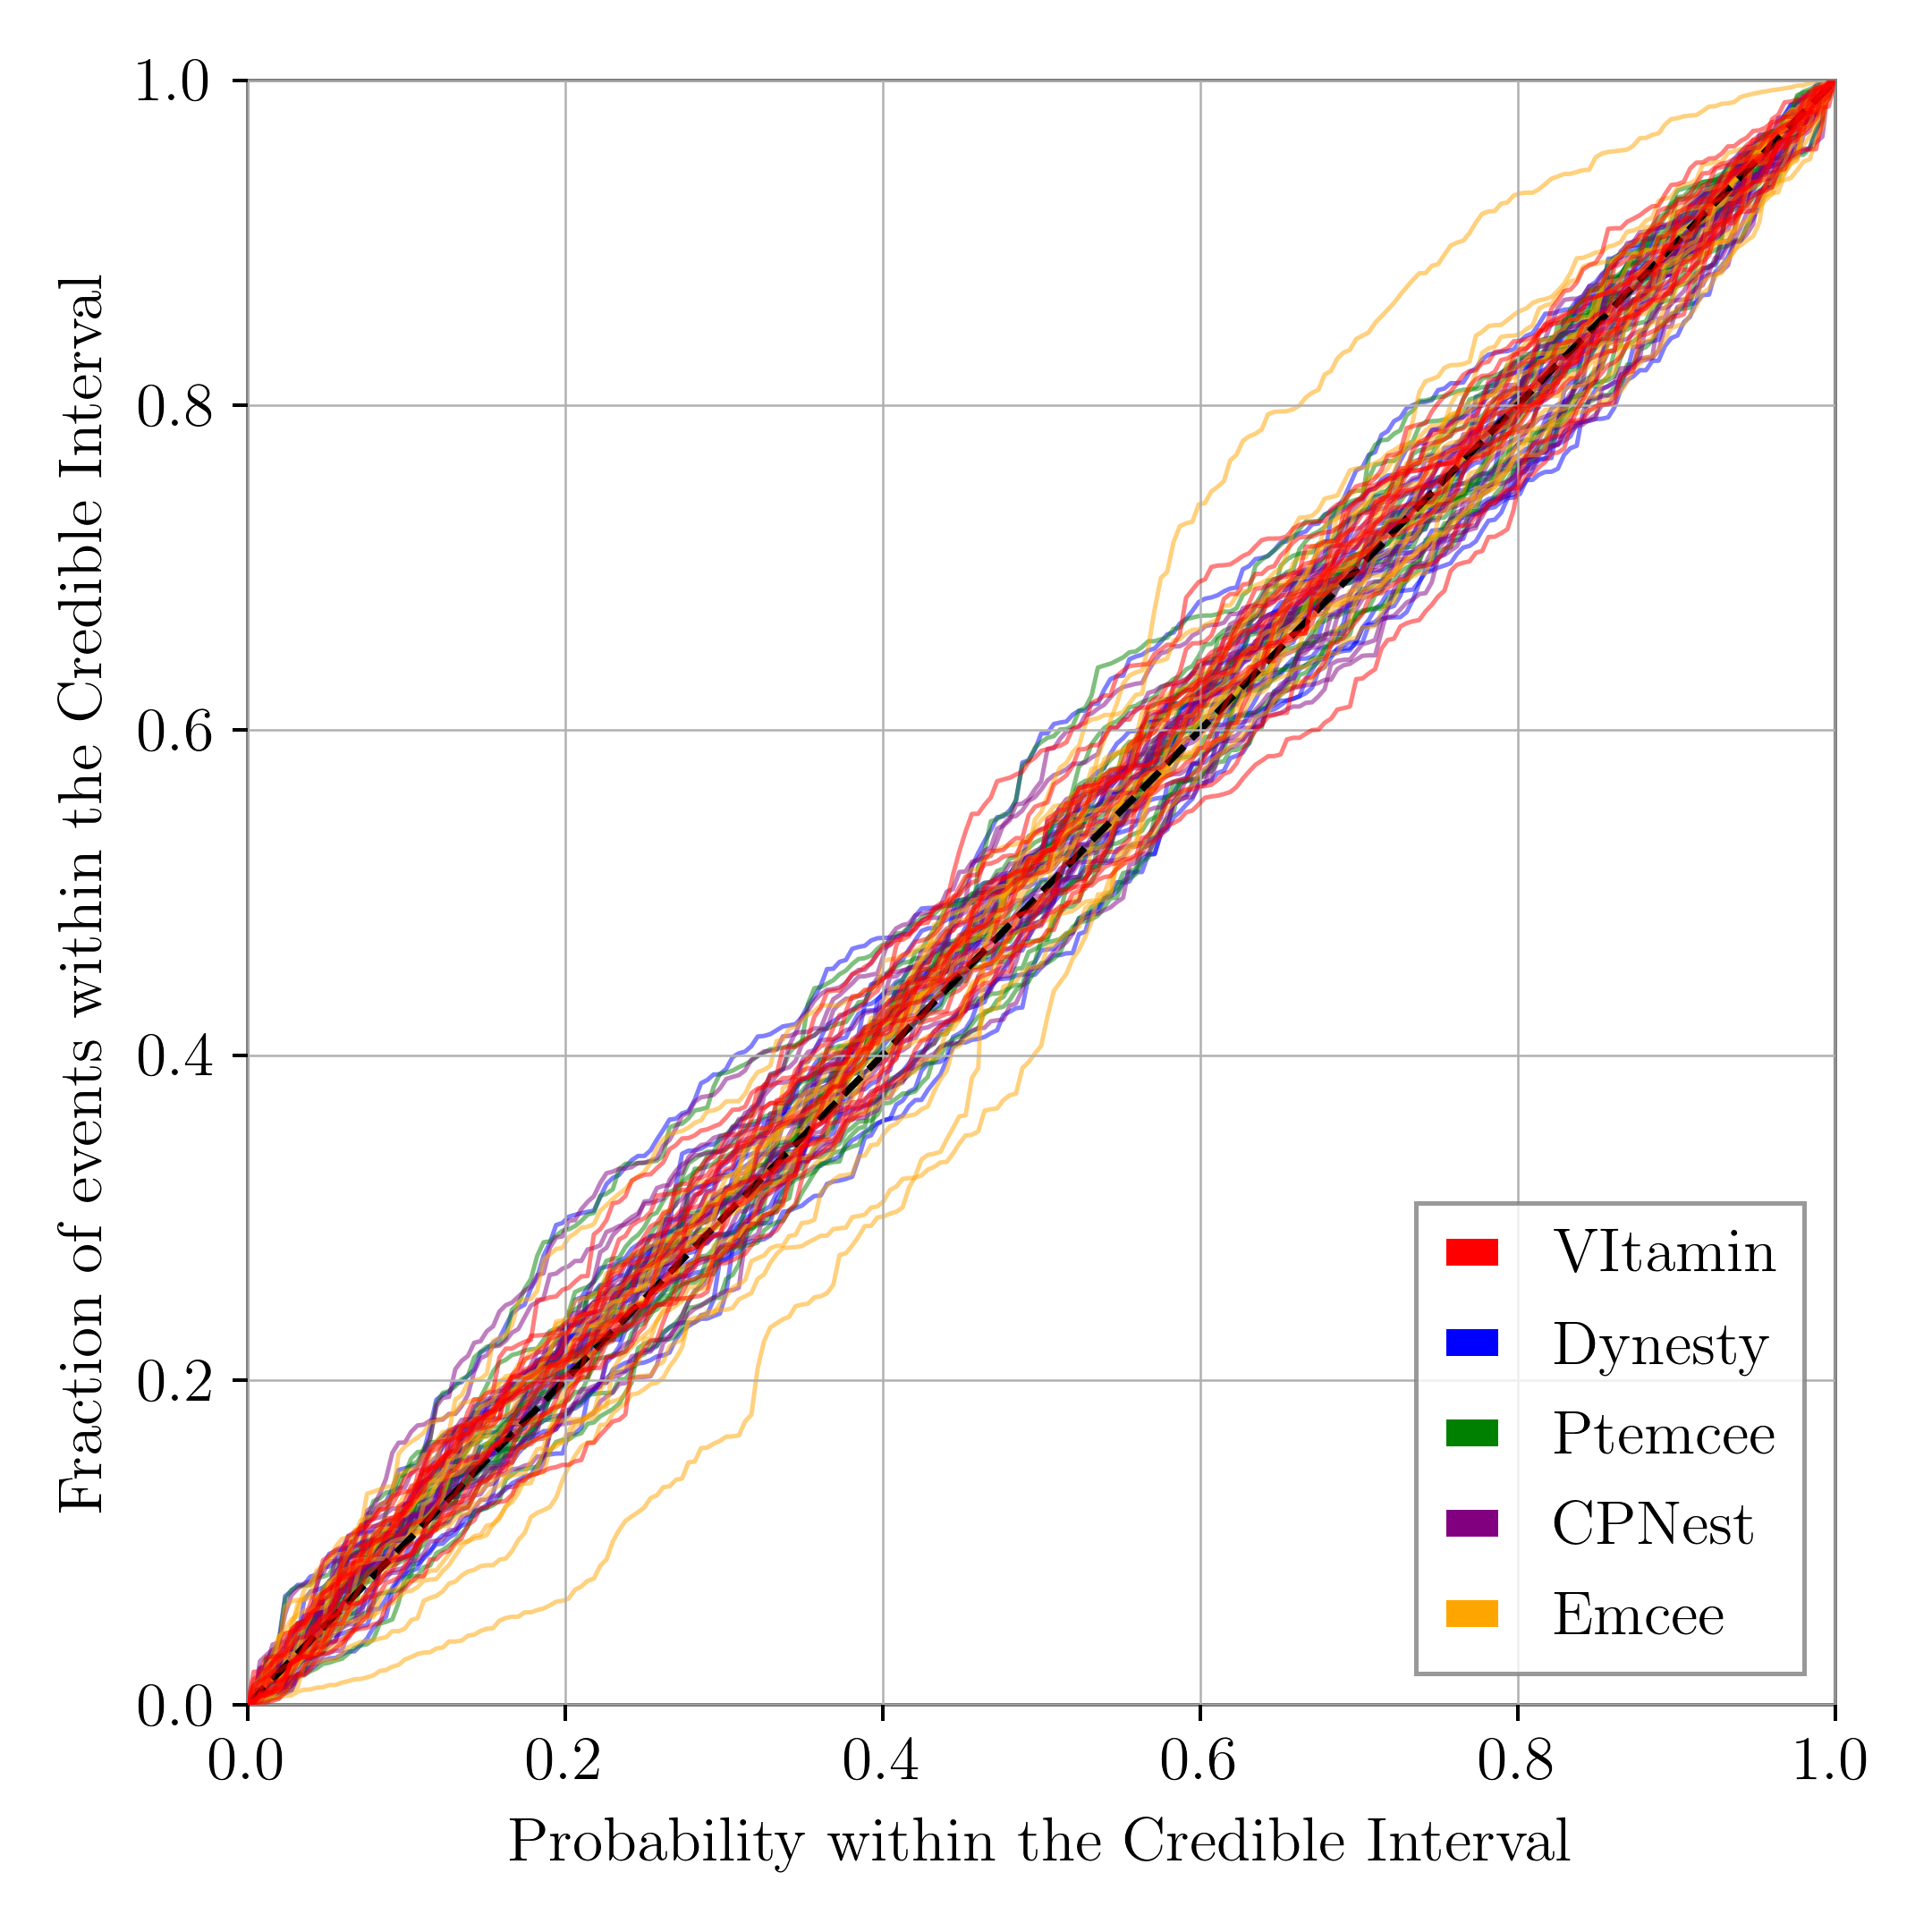
\includegraphics[width=\columnwidth]{latest_pp_plot.png}
    \caption{\label{fig:pp_plot} One-dimensional \ac{PP} plots for each
parameter and each benchmark sampler and \texttt{VItamin}.  The curves were
constructed using the 256 test datasets. The dashed black diagonal line
indicates the ideal result.
}
\end{figure}
%

%
% discuss pp plot result
%
%\chris{You need to better describe what a P-P plot is and why we use it. Maybe
%throw in a reference to existing PE group papers that use it. Nature readers
%will have never seen one before. We also have to wait until we get better P-P
%plot curves for our approach before we warrant adding it to the paper.}
A standard test used within the \ac{GW} parameter estimation community is the
production of so-called \ac{PP} plots which we show for our analysis in
Fig.~\ref{fig:pp_plot}. The plot is constructed by computing a $p$-value for each
output test posterior on a particular parameter evaluated at the true
simulation parameter value (the fraction of posterior samples $>$ the
simulation value). We then plot the cumulative distribution of these
values~\cite{1409.7215}. Curves consistent with the black dashed diagonal line
indicate that the 1-dimensional Bayesian probability distributions are
consistent with the frequentist interpretation - that the truth will lie within
an interval containing $X\%$ of the posterior probability with a frequency of
$X\%$ of the time. It is clear to see that our new approach shows deviations
from the diagonal that are entirely consistent with those observed in all
benchmark samplers. 

%
\begin{figure}
    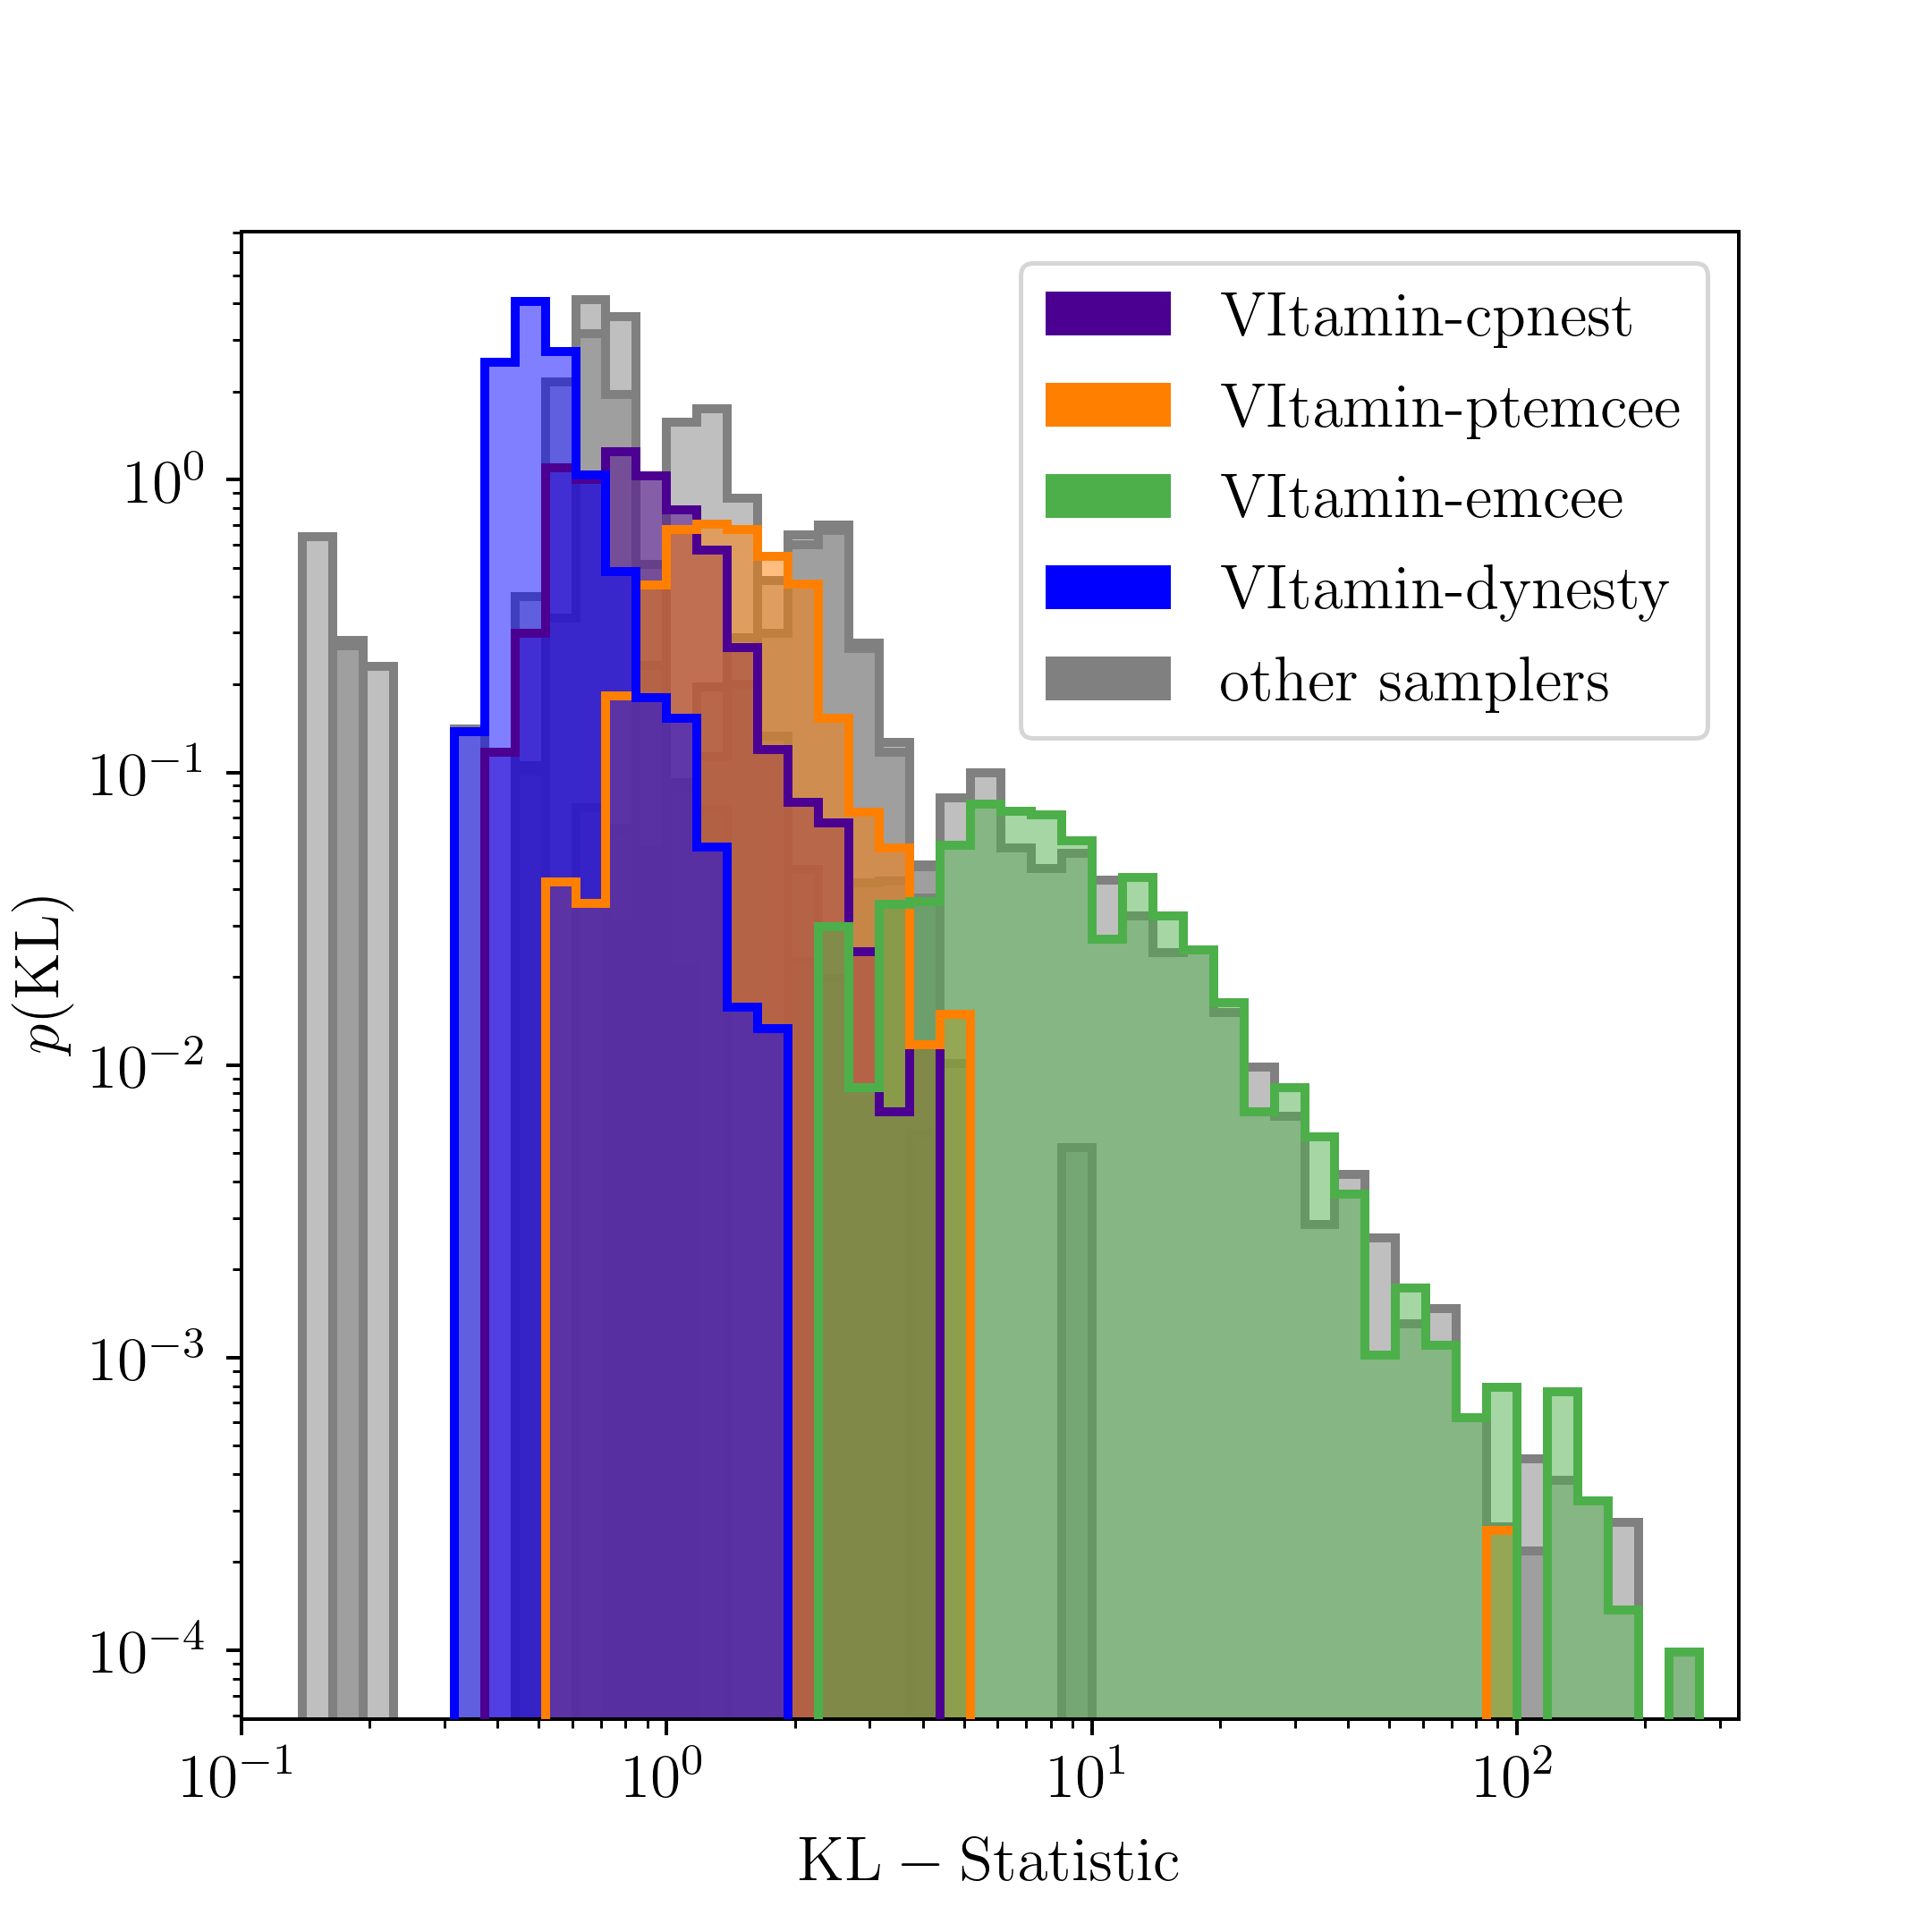
\includegraphics[width=\columnwidth]{hist-kl.png}
    \caption{\label{fig:kl_results} Distributions of \ac{KL}-divergence values
between posteriors produced by different samplers. The \ac{KL} divergence is
computed between all samplers with every other sampler over all 256 \ac{GW}
test cases. The distributions of the resulting \ac{KL} divergence values are
then plotted, with each color representing a different sampler combination
including \texttt{VItamin} as one of the sampler pairs. The grey distributions
represent the results from all benchmark sampler pairs for comparison. Both the
$x$ and $y$ axes are scaled logarithmically for readability.}
\end{figure}
%

%
% discuss the KL results
%
The \ac{KL} divergence between 2 distributions is a measure of their similarity
and we use this to compare the output posterior estimates between samplers for
the same input test data. To do this we run each independent sampler (including
the \ac{CVAE}) on the same test data to produce samples from the corresponding
posterior. We then compute the \ac{KL}-divergence between output distributions
from each sampler with itself and each sampler with all other samplers. For
distributions that are identical the \ac{KL}-divergence is equal to zero but
since we are representing our posterior distributions using finite numbers of
samples, identical distributions should result in KL-divergence values $<1$. In
Fig.~\ref{fig:kl_results} we show the distributions of these
\ac{KL}-divergences for the 256 test \ac{GW} samples where we see that the
\ac{CVAE} approach when compared to the benchmark samplers have distributions
consistent with those produced when comparing between 2 different benchmark
samplers.


\chapter{Conditional variational autoencoders for detecting real GW signals}

In this chapter I will discuss some recent soon to be published work on using the \texttt{VItamin} machine learning for gravitational wave parameter estimation pipeline to do Bayesian PE on real \ac{GW} signals. In the first section I will introduce the problem, in the second I will discuss data pre-processing and generation, in the third section I will discuss results in both real and Gaussian noise cases on a variety of real \ac{GW} signals.

\section{Introduction}

\section{Signal pre-processing/generation}

\section{Results}

\section{Conclusions}


\chapter{Conclusions}


%%
% Extra sections required for progression report
%

\chapter{Thesis outline}

\section{Background chapter on GWs}

In this chapter I will discuss the most relevant general relativity concepts with regards to gravitational waves. There will be a very brief description of the LIGO detector configuration including some discussion on how non-astrophysical noise affects the data quality coming out of the detectors. I will end by describing the most widely used techniques in LIGO for both detecting and estimating the source parameters of gravitational wave events.

\section{Background chapter on machine learning}

Start out by providing some successful use-cases of machine learning and motivation for why machine learning is applicable to gravitational wave data analysis. Discuss the basics of machine learning from first principals (i.e. perceptron to deep neural networks). Discuss basics of the two types of networks used in the thesis (i.e. convolutional neural networks and conditional variational autoencoders).

\section{Chapter on matching matched filtering using convolutional neural networks for gravitational wave astornomy}

This will be a near copy and paste of our first paper published in Physical Review Letters on the use of convolutional neural networks to match the efficiency of the standard LIGO detection method matched template filtering. Most of the material is already here for this.

\section{Chapter on Bayesian parameter estimation using conditional variational autencoders for gravitational wave astronomy}

This will be a near copy and paste of our most recent paper (submitted to Nature Physics) where we show for the first time that a machine learning algorithm (conditional variational autoencoders) can reproduce Bayesian gravitational wave source parameter posterior estimates with a 7 order of magnitude increase in speed. Most of the material is already here for this.

\section{Technical chapter on matching matched filtering paper}

A more in-depth discussion on the techniques used in our PRL paper. This may include further expansion on application of training techniques, deeper discussion the strengths and weaknesses of the technique and a more nuanced explanation of what is going on inside of the network. Much of the work already carried out can be added to this chapter, though it may require an additional few months of analysis.

\section{Technical chapter on Bayesian PE using CVAE paper}

A more in-depth discussion on the techniques used in our Nature Physics paper. This may include further expansion on application of training techniques, deeper discussion the strengths and weaknesses of the technique and a more nuanced explanation of what is going on inside of the network. Much of the work already carried out can be added to this chapter, though it may require an additional month or two of analysis.

\section{Conclusions / discussion chapter}

A recap of what was done over the course of the entire thesis. Some discussion what could be done next and what was done wrong. The analysis for both technical chapters will need to be finished prior to the completion of the conclusions chapter.

%
% List of objections in second year progress report
%

\chapter{List of objectives in second year report}

\begin{itemize}
    \item \textbf{Achieve $95$ - $100\%$ overlap with the toy sine-Gaussian test case:} This was not achieved as we ended up finding a better method than generative adversarial networks (i.e. conditional variational autoencoders). Our figure of merit has also changed from overlap to KL divergence and we have moved on from the toy model case.
    \item \textbf{Achieve $90$ - $100\%$ overlap with the gravitational wave test case:} This has largely been achieved in our most recent paper using a new method and with a different figure of merit (i.e. KL divergence).
    \item \textbf{Write and publish paper on INN applied towards GW parameter estimation:} This has largely been achieved. We are not using invertible neural networks anymore (now using conditional variational autoencders) and we have written up and submitted the paper to Nature Physics. Currently in the refereeing stage.
    \item \textbf{Complete 6-month placement at Craft Prospect company:} This has been done and I even received a job offer out of it.
    \item \textbf{Do a more in-depth analysis of previous results from both GAN and CNN study:} We have not had the time to do this yet (as we have been busy trying to get this Nature paper out), but will finish this up in the coming year.
    
\end{itemize}

\chapter{List of objectives and outline plan for next 12 months}

\begin{itemize}
    \item Resubmit paper to Nature Physics with comments to referees.
    \item Perform further technical analysis on matching matched filtering paper.
    \item Perform further technical analysis on Bayesian parameter estimation CVAE paper.
    \item (Time dependent) Write up technical PRD paper on the further technical analysis performed above.
    \item Write thesis.
\end{itemize}



\backmatter  % Turn off chapter numbering
% I assume that the bibliography is assembled by hand.
% Change the file if you use bibtex or something like that.
%\begin{thebibliography}{99}
\addcontentsline{toc}{chapter}{Bibliography}
% Surely there is a better way than the line above

\bibitem{Bastard}
Bastard, G. (1988).
\textit{Wave mechanics applied to semiconductor heterostructures}.
New York: Halsted; Les Ulis: Les Editions de Physique.

\bibitem{Kelly}
Kelly, M. J. (1995).
\textit{Low-dimensional semiconductors: materials, physics, technology, devices}.
Oxford: Oxford University Press.

\bibitem{Weisbuch}
Weisbuch, C., and Vinter, B. (1991).
\textit{Quantum semiconductor structures}.
Boston: Academic Press.

\end{thebibliography} 

\bibliographystyle{abbrv}
\bibliography{references}

\end{document}
